%--------------------------------
% praca dyplomowa
% Konrad Ziaja
% 2017
%--------------------------------


\documentclass[a4paper,12pt,twoside,openany]{report}
%
% Wzorzec pracy dyplomowej
% J. Starzynski (jstar@iem.pw.edu.pl) na podstawie pracy dyplomowej
% mgr. inż. Błażeja Wincenciaka
% Wersja 0.1 - 8 października 2016
%

%%%
% PAKIETY
%%%

\usepackage{polski}
\usepackage{helvet}
\usepackage[T1]{fontenc}
\usepackage{anyfontsize}
\usepackage[utf8]{inputenc}
\usepackage[pdftex]{graphicx}
\usepackage{tabularx}
\usepackage{array}
\usepackage[polish]{babel}
\usepackage{subfigure}
\usepackage{amsfonts}
\usepackage{verbatim}
\usepackage{indentfirst}
\usepackage[pdftex]{hyperref}
\usepackage{prmag2017}
\usepackage{todonotes} 
\usepackage{amsmath}
\usepackage{multirow}
\usepackage{enumitem}	% enumitem.pdf
\usepackage{float}

% rozmaite polecenia pomocnicze
% gdzie rysunki?
\newcommand{\ImgPath}{.}

% oznaczenie rzeczy do zrobienia/poprawienia
\newcommand{\TODO}{\textbf{TODO}}


% wyroznienie slow kluczowych
\newcommand{\tech}{\texttt}

% na oprawe (1.0cm - 0.7cm)*2 = 0.6cm
% na oprawe (1.1cm - 0.7cm)*2 = 0.8cm
%  oddsidemargin lewy margines na nieparzystych stronach
% evensidemargin lewy margines na parzystych stronach
\def\oprawa{1.05cm}
\addtolength{\oddsidemargin}{\oprawa}
\addtolength{\evensidemargin}{-\oprawa}

\setlist{listparindent=\parindent, parsep=\parskip} % potrzebuje enumitem
\let\oldtabular\tabular 
\renewcommand{\tabular}{\scriptsize\oldtabular}

    




%%%%%%%%%%%%%%% Strona Tytułowa %%%%%%%%%%%%%%%%%
% To trzeba wypelnic swoimi danymi
\title{Meta-metody służące do poprawy jakości klasyfikacji}

% autor
\author{Konrad Ziaja}
\nrindeksu{272170}

\opiekun{dr inż. Łukasz Skonieczny}
\rok{2017}
\terminwykonania{XX lutego 2017} % data na oświadczeniu o samodzielności




% To sa domyslne wartosci
% - mozna je zmienic, jesli praca jest pisana gdzie indziej niz w ZETiIS
% - mozna je wyrzucic jesli praca jest pisana w ZETiIS
\miasto{Warszawa}
\uczelnia{POLITECHNIKA WARSZAWSKA}
\wydzial{Wydział Elektroniki i Technik Informacyjnych}
\instytut{Instytut Informatyki}
\zaklad{Zakład Systemów Informacyjnych}
\kierunekstudiow{INFORMATYKA}
\specjalnosc{Inżynieria Systemów Informatycznych}

\pracamagisterska
%%% koniec od P.W

\opinie{%
	\input{opiniaopiekuna.tex}
	\newpage
	\input{recenzja.tex}
}

\streszczenia{
	\input{streszczenie.tex}
}
\begin{document}
\maketitle

\chapter*{Wstęp}
\addcontentsline{toc}{chapter}{Wstęp}
Ostatnie dekady to wielki skok cywilizacyjny. Nastąpił gwałtowny rozwój informatyki oraz pokrewnych dziedzin. Wskutek postępu technicznego, ludzie zaczęli generować ogromne ilości danych, które zostają zapisane na co raz większych i tańszych nośnikach danych. Codziennie, podczas zwykłych czynności np. płacenia kartą w sklepie, przeglądania internetu, wysyłania poczty e-mail, nosząc ze sobą podłączony do sieci GSM telefon tworzymy nieświadomie duże ilości danych. Firmy ubezpieczeniowe, banki, sklepy, sieci handlowe i inne instytucje prywatne oraz publiczne zbierają i przetwarzają o nas różne informacje, a następnie gromadzą je w ogromnych bazach danych. Dziedzinami zajmującymi się przetwarzaniem danych oraz wyszukiwaniem wzorców i wiedzy w danych jest uczenie maszynowe (ang. \textit{machine learning}) oraz eksploracja danych (ang. \textit{data mining}). Uczenie maszynowe można podzielić między innymi na uczenie nadzorowane (ang. \textit{supervised learning}) oraz uczenie nienadzorowane (ang. \textit{unsupervised learning}). W uczeniu nadzorowanym program dla znanych danych z przypisanymi klasami lub kategoriami tworzy reguły decyzyjne, które następnie wykorzystywane są do przypisania klasy nowym nieznanym wcześniej danym. Natomiast w uczeniu nienadzorowanym, wyszukiwane są wzorce, struktury w danych bez przypisanej końcowej kategorii. \par 
Elementem uczenia nadzorowanego jest klasyfikacja danych (ang. \textit{classification}). W procesie klasyfikacji danych, system wyszukuje wzorców oraz reguł w danych uczących ze znanymi kategoriami, a następnie przypisuje kategorię nowym obserwacjom bez określonej klasy. Oczywiście przypisana kategoria pochodzi ze zbioru danych uczących. Przykładem klasyfikacji danych może być proces przyznania kredytu. Bank zbiera różne informacje o klientach (rodzaj pracy, umowy, wysokość zarobków, poprzednie pożyczki, kredyty, terminowość spłat rat), a następnie po jakimś czasie oznacza czy był to dobry klient z korzyścią dla banku. Klasyfikator nauczony tymi danymi, określa czy można udzielić kredytu nowemu klientowi na podstawie dostarczonych danych. Innym przykładem mogą być dane medyczne np. osób chorych na raka. Lekarz gromadzi parametry medyczne pacjentów wraz z kategorią czy dana osoba jest chora. Na podstawie tych danych, tworzony jest model klasyfikacyjny, który pomaga określić czy nowy pacjent może być potencjalnie chory.\par 
Skuteczność klasyfikacji zależna jest między innymi od ilości i jakości danych oraz od klasyfikatora (algorytmu klasyfikującego). Istnieje wiele różnych algorytmów klasyfikacji, takich jak: drzewo decyzyjne, naiwny klasyfikator Bayesa, sieć neuronowa, maszyna wektorów nośnych oraz wiele innych. Algorytmy te osiągają różną skuteczność dla różnych danych. W celu poprawy skuteczności klasyfikacji można wykorzystać meta-metody, inaczej metauczenie (ang. \textit{meta learning}). Celem metauczenia jest poprawa skuteczności klasyfikacji istniejących algorytmów. Najczęściej wykorzystuje się przewidywania różnych klasyfikatorów, które łączy się tworząc metadane. Następnie meta-klasyfikator (główny klasyfikator) lub wszystkie klasyfikatory poprzez głosowanie decydują o końcowej klasie nowych obserwacji. 	\par 
Dane medyczne często zawierają dużą ilość osób zdrowych, a małą ilość osób chorych. Klasyfikując nowych pacjentów zależy nam na dużej skuteczności wykrywania osób potencjalnie chorych. Niestety, w przypadku dużego niezrównoważenia klas danych, klasyfikator często osiąga niską skuteczność klasyfikacji mniej liczebnej klasy. Aby poprawić wykrywalność mniejszej klasy stosuje się sztuczne równoważenie zbiorów lub zmodyfikowane algorytmy klasyfikacji.
\chapter*{Zakres i cel pracy}
\addcontentsline{toc}{chapter}{Zakres i cel pracy}
Celem pracy magisterskiej było zbadanie wpływu meta-metod (metauczenia) na poprawę jakości klasyfikacji danych oraz danych niezrównoważonych. Do badań wybrano algorytmy bagging, boosting oraz stacking. Wszystkie meta-metody miały zostać przetestowane z kilkoma podstawowymi algorytmami klasyfikacji. Klasyfikacja miała być przeprowadzona dla danych z różnych dziedzin, z rożną ilością przykładów i atrybutów oraz z różnym rozkładem klas. Ważnym elementem badań była klasyfikacja zbiorów niezrównoważonych, z wyraźną dominacją liczebną jednej klasy. We wstępnym przetwarzaniu danych, miały zostać użyte metody równoważące rozkład klas w zbiorze danych. Metody równoważenia klas danych, należało porównać i zbadać wpływ na proces klasyfikacji z meta-metodami. Ostatnim elementem niniejszej pracy była próba stworzenia uniwersalnego meta-klasyfikatora, uzyskującego wysoką jakość klasyfikacji dla większości zbiorów danych. \par
Zakres pracy stanowiło przetestowanie meta-metod. Gotowe algorytmy klasyfikacji miały pochodzić z biblioteki $scikit-learn$. Implementacja algorytmów klasyfikacji nie wchodziła w zakres pracy. Miały zostać napisane testy w języku $python$ badające, oceniające i porównujące meta-metody oraz wybrane klasyfikatory. Testy powinny zwracać otrzymane wyniki w postaci plików pdf. Ostatnim elementem było stworzenie meta-klasyfikatora. \par
Rozdział pierwszy i drugi stanowią wprowadzenie teoretyczne do problemu klasyfikacji oraz klasyfikacji danych niezrównoważonych. W rozdziałach tych opisana jest klasyfikacja, użyte algorytmy klasyfikacji oraz meta-metody. Czytelnik może zaznajomić się także z informacją w jaki sposób i z jakimi miarami ocenia się klasyfikację danych. W rozdziale poświęconym klasyfikacji danych niezrównoważonych, znajduje się geneza problemu oraz opis dostępnych i możliwych rozwiązań poprawy klasyfikacji takich danych. \par
Rozdział trzeci poświęcony jest opisowi platformy do badań oraz analizie użytych danych do klasyfikacji. Zostały także przetestowane i wybrane wiarygodne sposoby oceniania klasyfikatora oraz sposoby równoważenia zbiorów danych. \par
W rozdziale czwartym opisano przeprowadzone badania na meta-metodach. Przeprowadzono testy z różnymi algorytmami oraz ustawieniami klasyfikatorów. Część rozdziału przeznaczona została na poprawę klasyfikacji danych mniejszościowych. Przetestowano i porównano wybrane metody równoważenia klas w zbiorach wraz z meta-metodami. \par
W piątym rozdziale zaprezentowano zmodyfikowany pomysł głosowania, w postaci klasyfikatora eksperckie. Przedstawiono także projekt meta-klasyfikatora. Podobnie jak poprzednia, oba klasyfikatora zostały przetestowane z użyciem prawdziwych zbiorów danych. \par
W ostatnim rozdziale opisano uzyskane wyniki oraz podsumowanie całej pracy.

\chapter{Wstęp teoretyczny}
\section{Klasyfikacja danych}
\todo{może coś pisać o uczeniu maszynowym i że klasyfikacja moze byc nadzorowana i nie?} 

Klasyfikacja jest to proces przyporządkowania danych do jednej z predefiniowanych klas na podstawie atrybutów tych danych. Algorytm klasyfikacji na podstawie analizy danych trenujących, zawierających atrybuty oraz klasę, tworzy model klasyfikacyjny. Stworzony model klasyfikacyjny wykorzystywany jest do predykcji klasy (kategorii) nowych danych bez określonej klasy. Celem algorytmu budującego model, jest  odnalezienie wzorców, w jaki sposób atrybuty obiektu wpływają na przynależność do danej klasy, starając się o to, aby wiedza na temat analizowanych danych była możliwie ogólna oraz niezależna od próby.

Klasyfikacja danych jest procesem dwuetapowym:
\begin{itemize}
	\item budowa modelu – proces ten polega na analizie obiektów z przyporządkowaną klasą oraz na budowie modelu opisującego predefiniowany zbiór klas danych,
	\item właściwa klasyfikacja – otrzymany model stosuje się do przydzielania klasy nowym obiektom.
\end{itemize}
Budowa modelu jest także procesem dwu-etapowym. Dzieli się ona na:
\begin{itemize}
	\item uczenie – klasyfikator budowany jest w oparciu o dane treningowe,
	\item ocena jakości klasyfikacji – jakoś klasyfikacji badana jest w oparciu o dane testowe.
\end{itemize}
W zależności od liczebności klas w zbiorze danych, możemy wyróżnić:
\begin{itemize}
	\item klasyfikację binarną – klasyfikator decyduje o przypisaniu obiektu do jednej z dwóch klas (np. czy człowiek jest zdrowy lub nie)
	\item klasyfikację wieloklasową – obiektowi przypisuje się jedną z wielu predefiniowanych klas.
\end{itemize}
Do reprezentacji danych uczących, testowych oraz do klasyfikacji najczęściej stosuje się system informacyjny.
\begin{table}[h]
\begin{center}
	\resizebox{\textwidth}{!}{%
	\begin{tabular}{|c|c|c|c|c|c|l|}	
		\hline
		{\bf Zachmurzenie} & {\bf Temp.} & {\bf Temp. wody} & {\bf Opady} & {\bf Wiatr} & {\bf Pływać} & {\bf h(x)}\\
		\hline 
		słonecznie & 32 & 25 & brak & słaby & tak & tak \\
		\hline 
		słonecznie & 31 & 26 & brak & umiarkowany & tak & nie \\
		\hline
		pochmurnie & 22 & 15 & brak & b. mocny & nie & nie \\
		\hline
		pochmurnie & 20 & 18 & brak & słaby & tak & tak \\
		\hline
		całkowite zachmurzenie & 12 & 6 & brak & umiarkowany & nie & nie \\
		\hline
		całkowite zachmurzenie & 10 & 8 & duże & słaby & nie & nie \\
		\hline
		pochmurnie & 21 & 10 & brak & mocny & nie & tak \\
		\hline
		słonecznie & 25 & 17 & brak & umiarkowany & tak & nie \\
		\hline
		pochmurnie & 23 & 17 & przelotne & umiarkowany & nie & tak \\
		\hline
	\end{tabular}}
	\caption{Przykład danych treningowych składających się z 5 atrybutów oraz klasy decyzyjnej. W ostatniej kolumnie znajduje się wynik klasyfikacji. W pięciu przypadkach, klasyfikator poprawnie wskazał klasę.}
	\label{system_informacyjny}
\end{center}
\end{table}
\section{Wybrane algorytmy klasyfikacji danych}
\subsection{Drzewo decyzyjne}
Drzewo decyzyjne jest bardzo często wykorzystywane jako klasyfikator danych. Celem jest stworzenie modelu, który na podstawie danych wejściowych przewidzi poprawnie klasę. Drzewo jest acyklicznym spójnym grafem skierowanym. Korzeń (węzeł na poziomie 0) zawiera w sobie cały zbiór uczący. W każdym węźle przeprowadza się test na wartościach atrybutu, który dzieli zbiór nad podzbiory. Z węzła wychodzi tyle gałęzi ile jest możliwych wyników testu z tego węzła. Pod każdym węzłem znajduje się kryterium podziału dokonywanego w danym węźle, które jest jednakowe dla wszystkich elementów zbioru. Ostatnim elementem drzewa decyzyjnego są liście, które zawierają etykiety, czyli przydział klasowy elementów z tego podzbioru. Drzewo buduje się w sposób rekurencyjny od korzenia do liścia z wykorzystaniem metody "dziel i zwyciężaj".\\
\subsubsection{Proces budowy drzewa}
\begin{enumerate}
	\item Stwórz korzeń zawierający cały zbiór uczący.
	\item Jeśli wszystkie przykłady należą do tej samej klasy decyzyjnej, to węzeł staje się liściem z etykietą klasy.
	\item Jeżeli nie, oblicz kryterium podziału wykorzystując np. entropię, które najlepiej dzieli zbiór treningowy.
	\item Dla każdego testu stwórz gałąź i podziel odpowiednio podzbiory do nowych węzłów.
	\item Wywołaj rekurencyjne algorytm dla nowych węzłów.
	\item Algorytm kończy się dla kryterium stopu.
\end{enumerate}
Stosuje się różne kryterium stopu:
\begin{itemize}
	\item wszystkie przykłady należą do tej samej klasy,
	\item brak możliwości dalszego podziału,
	\item zbiór pusty,
	\item osiągnięto zakładany cel, np.: maksymalna głębokość drzewa, maksymalna czystość klas w liściu, minimalny przyrost informacji po podziale.
\end{itemize}

Jako kryterium podziału można stosować np. wskaźnik Giniego lub entropię. Często zdarza się, że zbudowane drzewa są zbyt duże i tworzy się nadmierne dopasowanie do danych. Wtedy powinno ograniczyć się wysokość drzewa.
Istnieje kilka algorytmów drzew decyzyjnych takich jak: ID3, C4.5, CART, CHAID. 
\todo{wstawic obrazek drzewa decyzyjnego} 
\subsection{Naiwny klasyfikator bayesowski}
Naiwny klasyfikator bayesowski opiera się na twierdzeniu o prawdopodobieństwie warunkowym stworzonym przez Thomasa Bayesa. Jest to klasyfikator probabilistyczny, zwracający prawdopodobieństwo przynależności przykładu do danej kategorii. Liczba kategorii musi być skończona i zdefiniowana a priori. Zasada działania klasyfikator opiera się na twierdzeniu:
\[P(C_i|x) = \frac{P(x|C_i)P(C_i)}{P(x)}\]
gdzie:
\begin{itemize}
	\item $x$ - przykład dla którego nieznana jest klasa, jest to n-wymiarowy wektory, a n oznacza liczbę atrybutów,  
	\item $P(C_i|x)$ - prawdopodobieństwo a posteriori, że przykład x należy do klasy $C_i$,
	\item $P(x|C_i)$ - prawdopodobieństwo a priori, że przykład x należy do klasy $C_i$,
	\item $P(C_i)$ - prawdopodobieństwo, że dowolny przykład należy do klasy $C_i$
	\item $P(x)$ to prawdopodobieństwo a priori wystąpienia przykładu x.
\end{itemize}
Działanie naiwnego klasyfikatora bayesowskiego oparte jest na założeniu, że atrybuty wewnątrz klasy są od siebie niezależne. Bardzo często to założenie nie jest spełnione, co rzutuje na wyniki osiągane przez ten klasyfikator oraz pokazuje genezę pochodzenia nazwy klasyfikatora.
\subsection{Klasyfikator k najbliższych sąsiadów (kNN)}
\todo{moze wstawic obrazek?}
Klasyfikator k najbliższych sąsiadów lub klasyfikator k-NN, (ang. \textit{k nearest neighbours}) należy do grupy algorytmów leniwych (ang. \textit{lazy learners}), które nie wymagają uczenia, a całe obliczenia wykonywane są w momencie pojawienia się wzorca testowego, czyli podczas klasyfikacji lub testowania. \\
Klasyfikacja nowego obiektu $x$ odbywa się poprzez znalezienie $k$ najbliższych sąsiadów w danych uczących $X$ i nadaniu mu nowej klasy poprzez głosowanie większościowe sąsiadów. Odległość pomiędzy sąsiadami można obliczyć np. takimi miarami jak: euklidesowa, Manhattan, Czebyszewa lub Minkowskiego. \\
Dobranie idealnej wartości parametru $k$ ma bardzo duże znaczenie w jakości klasyfikacji. Dobrze dobrane $k$ powinno być na tyle duże, aby minimalizować prawdopodobieństwo błędnych klasyfikacji, ale jednocześnie małe, aby $k$ najbliższych sąsiadów było rzeczywiście bliskimi sąsiadami testowanej obserwacji \cite{Bishop}. 
\subsection{Las losowy}
\todo{Jest to jeden z elementów bagging, może wspomnieć, albo dać w innym miejscu?}
Las losowy (ang. \textit{random forest}) lub losowe drzewa decyzyjne to klasyfikator złożony z drzew decyzyjnych. Algorytm trenujący działa według następującego schematu:
\begin{enumerate}
	\item Wylosuj metodą boostrap (losowanie ze zwracaniem) $n$ elementów ze zbioru danych,
	\item Zbuduj drzewo decyzyjne, w każdym węźle:
	\begin{itemize}
		\item wylosuj $d$ atrybutów,
		\item dla wylosowanych atrybutów, dokonaj najlepszego podziału (np. używając entropii, lub współczynnika Giniego).
	\end{itemize}
	\item Powtórz punkt 1 i 2 $k$ razy (gdzie k, to liczba drzew).
\end{enumerate}
Każde drzewo klasyfikuje przykład, a ostateczna klasa nadawana jest poprzez głosowanie większościowe. \\
Zazwyczaj, im większa liczba drzew $k$ tym lepsze wyniki można otrzymać. Zmieniając liczbę losowanych przykładów $n$ do zbioru uczącego, można kontrolować wariancję błędu. Im $n$ większe, tym las losowy ma większą tendencję do nadmiernego dopasowania. Zmniejszając liczbę losowanych obserwacji można zmniejszyć szansę na przeuczenie i podnieść jakość klasyfikacji. Zazwyczaj $n$ równa się wielkości zbioru danych. Liczbę losowanych atrybutów $d$, zwykle przyjmuje się na poziomie $d = \sqrt{m}$, gdzie $m$ to ilość wszystkich atrybutów.
\subsection{Maszyna wektorów nośnych}
\todo{wstawic obrazek SVMA}
Maszyna wektorów nośnych, SVM (ang. \textit{support vector machine}) jest to nieprobabilistyczny, binarny, liniowy klasyfikator. Zbudowany model SVM, określa do której z dwóch klas należą dane wejściowe. Konstrukcja klasyfikatora opiera się na znalezieniu hiperpłaszczyzny  w przestrzeni wielowymiarowej oddzielającej dwie klasy zbioru uczącego. Zadaniem algorytmu jest wybór tej z możliwie największym marginesem, tak aby odległość najbliższych punktów po obu stronach była największa. Oddzielająca hiperpłaszczyzna, opisana jest z wykorzystaniem wektora normalnego. Wektor ten jest liniową kombinacją najbliższych do hiperpłaszczyzny punktów. Jakość klasyfikacji zależy od szerokości granicy rozdzielającej klasy, im jest większa, tym błąd uogólnienia powinien być mniejszy. Modele z małym marginesem mogą wykazywać nadmierne dopasowanie. Klasyfikacja właściwa nowych przypadków, polega na określeniu po której stronie marginesu znajduje się nowy punkt i na tej podstawie wyznaczana jest klasa. \\
Istnieje modyfikacja podstawowego algorytmu, dla przypadku, gdy nie istnieje hiperpłaszczyzna oddzielająca dwie klasy. Jest to maszyna wektorów nośnych o miękkim marginesie. Bierze ona pod uwagę możliwość występowania zaszumionych danych. Klasyfikator w procesie uczenia, szuka możliwie najlepszej hiperpłaszczyzny oddzielającej obie klasy. Stopień błędnej klasyfikacji mierzony jest poprzez zmienną rozluźniającą (ang. \textit{slack variable}). Zmienną tą można traktować jako karę, dla danych znajdujących się po złej stronie granicy. Można ją kontrolować poprzez parametr C, który decyduje o szerokości rozdzielającego marginesu. Duża wartość parametru C, oznacza wysokie kary za błędną klasyfikację. \\
Jeżeli problem jest nieseparowalny  liniowo, można zastosować tzw. trik jądra, który polega na zastąpieniu liniowego jądra, nieliniowym. Pozwala to na stworzenie klasyfikatora nieliniowego. Najczęściej stosuje się następujące jądra:
\begin{itemize}
	\item wielomianowe (ang. \textit{polynomial})
	\item potencjalnych funkcji bazowych RBF (ang. \textit{radial basis function})
	\item sigmoidalne
\end{itemize}

  	
\subsection{Zespół klasyfikatorów}
W celu poprawy jakości klasyfikacji, można zastosować zespół klasyfikatorów w celu przypisania kategorii nowemu przykładowy. Zespół taki może składać się z kilku klasyfikatorów o takich samych algorytmach lub różnych. Jeżeli są to takie same klasyfikatory, to każdy model uczony jest na innych danych. Dla każdego modelu, dane trenujące mogą być wyznaczane poprzez losowanie lub losowanie ze zwracaniem. Zwykle zbiór trenujący przyjmuje nie więcej niż 2/3 wszystkich elementów. Możliwe jest także, podzielenie zbioru trenującego na $k+1$ (gdzie k to liczba klasyfikatorów) części i przekazanie każdemu klasyfikatorowi różnych $k$ części jako zbiór trenujący. Innym sposobem jest modyfikacja przestrzeni atrybutów. Każdy z klasyfikatorów otrzymuje zbiór danych zawierający inne atrybuty. \\
Jeżeli są to różne algorytmy, to wszystkie modele można uczyć na takich samych danych. \\
Każdy klasyfikator otrzymuje nowy przykład i nadaje mu kategorię. Ostateczna kategoria wyznaczana jest poprzez:
\begin{itemize}
	\item głosowanie większościowe (ang. \textit{majority voting}) wybierana jest klasa najczęściej wskazywana przez modele,
	\item głosowanie ważone (ang. \textit{weighted voting}) każdy klasyfikator ma przypisaną wagę lub zamiast predykcji klasy, zwraca prawdopodobieństwo z jakim przewiduje daną klasę. Docelową klasą jest ta wyliczonym największym prawdopodobieństwem.
\end{itemize} 
\section{Meta-metody}
\subsection{Bagging}
Metoda bagging  jest znana także jako bootstrap aggregating to zespół klasyfikatorów, meta-algorytm pozwalający zmniejszyć wariancję oraz uniknąć nadmiernego dopasowania. Metoda ta została zaproponowana w 1994 przez Leo Breiman’a w celu podniesienia jakości klasyfikacji poprzez połączenie wielu klasyfikatorów tego samego typ uczących się na losowym zbiorze danych. Zbiór uczący dla każdego klasyfikatora tworzy się poprzez losowanie ze zwracaniem z głównego zbioru danych. Losowanie wykonuje się z rozkładem jednostajnym. Nowo tworzony zbiór może być mniejszy lub takiej samej wielkości. Jeżeli zbiór danych jest duży i wygenerowany zbiór ma taką samą wielkość, można spodziewać się $1-\frac{1}{e}$ (około 63,2\%) unikalnych próbek. Takie losowanie nosi nazwę próby bootstrap. Zazwyczaj łączy się wyniki wielu modeli tego samego typu. Mając zbiór uczący $D$ o rozmiarze $n$, algorytm wygląda następująco:
\begin{enumerate}
	\item Wygeneruj $m$ nowych zbiór treningowych $D_i$, o rozmiarze $n'$, poprzez losowanie ze zwracaniem ze zbioru $D$,
	\item Trenuj $m$ klasyfikatorów w oparciu o wygenerowane zbiory treningowe $D_i$.	
\end{enumerate}
Nowa próbka klasyfikowana jest przez wszystkie modele, a ostateczna klasa nadawana jest poprzez głosowanie większościowe.
W metodzie bagging bardzo ważny jest dobór odpowiedniego klasyfikatora oraz zastanowienie się czy ta metoda może podnieść dokładność klasyfikacji. Jeżeli klasyfikator jest niestabilny (np. mała zmiana w danych treningowych powoduję zmianę dokładności klasyfikatora) metoda bagging może znacząco podnieść jakość i dokładność klasyfikacji. Jeżeli jednak klasyfikator jest stabilny, stosowanie metody bagging może doprowadzić do zmniejszenia jakości klasyfikacji z powodu zmniejszenia ilości danych treningowych.
\subsection{Boosting}
W 1988 i 1989 roku Micheal Kearns oraz Leslie Valiant postawili pytanie czy można stworzyć zbiór słabych klasyfikatorów, w celu stworzenia jednego silnego. Słaby klasyfikator to taki, który osiąga tylko minimalnie lepsze wyniki od losowania (zgadywania). Natomiast dobry klasyfikator osiąga wyniki mocno skorelowane z rzeczywistą klasyfikacją. W 1996 roku, Robert Schapire oraz Yoav Freund zaprezentowali algorytm AdaBoost. Istnieje dużo różnych algorytmów boostingu. 
Metoda boosting to zbiór klasyfikatorów, meta-algorytm, w którym w odróżnieniu od baggingu, słabe klasyfikatory budowane są sekwencyjnie. Większość algorytmów boostingu działa według następującego algorytmu:
\begin{enumerate}
	\item Każdemu przykładowi ze zbioru początkowego przypisywana jest taka sama waga początkowa, zazwyczaj $\frac{1}{n}$.
	\item Budowany jest nowy klasyfikator $m$ w oparciu o zbiór z wagami.
	\item Zbudowany klasyfikator dołączany jest do klasyfikatorów $M$ z wagą odpowiadającą jego dokładności.
	\item W zbiorze trenującym, następuje aktualizacja wag. Przykładom poprawnie sklasyfikowanym zmniejsza się wagę, natomiast  błędnie sklasyfikowanym zwiększa się.
	\item Punkt 2-4 powtarzany jest do momentu osiągnięcia liczby estymatorów $m$ lub do osiągnięcia zakładanego błędu. 
\end{enumerate}
Takie podejście nazywa się boosting by weighting, w procesie uczenia bierze udział cały zbiór. Istnieje także boosting by sampling, w którym zbiór jest ograniczony do $n$ elementów, a zamiast wag, używa się prawdopodobieństwa. Zwiększając prawdopodobieństwo przykładów źle sklasyfikowanych, zwiększa się szansę na wylosowanie, a w konsekwencji na poprawną klasyfikację przez model. \\
Algorytm boosting, skupia się na przykładach błędnie klasyfikowanych. Pozwala znacząco poprawić jakość klasyfikacji w przypadku użycia słabych klasyfikatorów (skuteczność klasyfikacji niedużo powyżej 50\%). W przypadku klasyfikatorów osiągających lepsze wyniki, nie obserwuje się znaczącego przyrostu skuteczności. Boosting może wykazywać także, nadmierne dopasowanie do przykładów wielokrotnie źle klasyfikowanych. \\
W 2008 roku Phillip Long (Google) oraz Rocco A. Serveido (Uniwersytet Columbia), podczas 25. Międzynarodowej Konferencji poświęconej systemom uczącym, opublikowali artykuł, w którym zasugerowali, że większość stosowanych współcześnie algorytmów opartych o boosting jest wadliwa. Stwierdzili, że algorytmy AdaBoost, LogiBoost mogą wykazywać słabą odporność na losowy szum klasyfikacyjny, a zastosowanie ich w realnym świecie jest wielce wątpliwe. W artykule przedstawiony został przykład, w którym stwierdzono, że jeżeli część danych treningowych będzie miała źle oznaczone klasy, to algorytm nie będzie mógł poprawnie sklasyfikować tych danych. Skutkiem czego stworzenie modelu z dokładnością większą niż $\frac{1}{2}$ będzie niemożliwe. \\
Istnieje dużo algorytmów korzystających z metody boosting. Najpopularniejsze z nich to AdaBoost, LPBoost, TotalBoost, BrownBoost, MadaBoost, LogitBoost.
\subsection{Stacking}
Metoda stacking (kontaminacja modeli) to połączenie kilku lub kilkunastu klasyfikatorów o różnych algorytmach. W pierwszym etapie, klasyfikatory trenowane są na tych samych danych. Następnie zbiór treningowy klasyfikowany jest przez te modele, a przewidziane klasy tworzą nowy zbiór uczący dla meta-klasyfikatora. Zbiór treningowy można utworzyć także, z połączenia danych wejściowych z predykowanymi klasami. Zamiast klas, jako dodatkowe wejście, można użyć prawdopodobieństwa danej klasy, o ile wszystkie klasyfikatory wspierają tą funkcję. Meta-klasyfikatorem może być każdy algorytm. Bardzo często do tego celu stosuje się jednowarstwową regresję logistyczną lub sieć neuronową. 
\section{Klasyfikacja danych niezrównoważonych}
Większość istniejących algorytmów klasyfikacji, nastawiona jest na poprawną klasyfikację zbiorów o zrównoważonej liczebności wszystkich klas. Niestety w rzeczywistych problemach, bardzo często zdarza się, że zbiory są mocno niezbilansowane.
\subsubsection{Dane niezrównoważone}
\todo{dodac odnosnik do one vs all}
Dane są niezrównoważone (ang. \textit{imbalanced data} jeśli klasy decyzyjne nie są przybliżeniu tak samo liczebne. Najmniejsza klasa, nazywana jest klasą mniejszościową (ang. \textit{minority class}), natomiast klasa dominująca, lub pozostałe połączone klasy (można połączyć pozostałe klasy w jedną, doprowadzając do klasyfikacji binarnej, one vs all), nazywana jest klasą większościową (ang. \textit{majority class}). W praktyce klasa mniejszościowa, zazwyczaj liczy około 10-20\% wszystkich przykładów. Często zdarzają się jednak takie problemy, gdzie to zróżnicowanie jest większe np.:
\begin{itemize}
	\item około 2\% transakcji kartami kredytowymi w GOCARDLESS to oszustwa \cite{gocardless}.

\end{itemize}
\todo{dodac przyklady danych mniejszosciowych}
W przytoczonych przykładach ważniejsza jest klasa mniejszościowa i wykrycie jej stanowi priorytet. Niezrównoważenie klas w zbiorze danych stanowi problem w fazie uczenia i znacząco obniża jakość klasyfikacji. Ze względu na częstość występowania klasy dominującej, klasyfikator preferuje tą klasę, dążąc do optymalizacji i obniżenia błędu error rate (\ref{error_rate}) nie biorąc pod uwagę rozłożenia klas w zbiorze. Klasyfikator może osiągnąć wysoką skuteczność klasyfikacji np. 95\% przy niskiej lub zerowej wykrywalności klasy mniejszościowej. 
Należy oczekiwać od klasyfikatora wysokiej skuteczności wykrywania klasy mniejszościowej, nawet kosztem pogorszenia rozpoznawania klasy większościowej.
Poddając analizie sąsiedztwa przykłady z klasy zdominowanej, można wyróżnić przykłady bezpieczne i niebezpieczne w klasyfikacji:
\begin{itemize}
	\item safe - przykład bezpieczny, w jego sąsiedztwie zdecydowana większość obserwacji jest z tej samej klasy,
	\item borderline - graniczny, przykład niebezpieczny, w jego sąsiedztwie ilość przykładów z obu klas jest podobna
	\item outlier - poboczny, przykład niebezpieczny, w jego sąsiedztwie większość obserwacji jest z klasy przeciwnej, dominującej,
	\item rare - rzadki, przykład niebezpieczny, w jego sąsiedztwie występują tylko przykłady z klasy przeciwnej, większościowej.
\end{itemize}
\todo{dodac obrazek danyych safe border itd.}
\todo{podac wykresy przykłady danych niezrównoważonych}

 
\section{Wstępne przetwarzanie danych}
\subsection{Brakujące wartości atrybutów}
Często zdarza się, że bazy danych nie są kompletne, że brakuje kilku wartości różnych atrybutów. Brakujące wartości mogą być wynikiem błędu człowieka, aplikacji, programu pomiarowego, nie podania danych lub z innego powodu. Zazwyczaj brakujące dane oznaczone są pustymi polami,? lub w inny opisany sposób. Istnieje kilka sposobów na rozwiązanie tego problemu.
\subsubsection{Usunięcie niekompletnych obserwacji}
Najprostszym sposobem jest usunięcie wierszy lub kolumn, w których brakuje wartości. Przed usunięciem, należy przeanalizować dane, sprawdzić, które usunięcie będzie najbardziej korzystne (usunie najmniej danych). Może bowiem zdarzyć się, że zamiast usuwać dużą ilość przykładów (wiersze), bardziej opłaca usunąć się atrybut (kolumnę), który ma dużo pustych komórek. Opisana metoda niesie ze sobą niepożądane konsekwencje. Usuwając, niektóre obserwacje lub atrybuty, pozbywa się części informacji. Skutkiem tego zabiegu model predykcyjny może działać słabiej. Następstwem stosowania tego sposobu jest także, w przyszłości brak możliwości predykcji niekompletnych przykładów.
\subsubsection{Imputacja danych}
Innym pomysłem na rozwiązanie tego problemu jest imputacja danych. Brakujące dane można obliczyć lub wyznaczyć różnymi technikami na podstawie wartości pozostałych obserwacji. Jeżeli atrybut zawiera wartości ciągłe, brakujące elementy można zastąpić wartością średnią lub medianą całej kolumny. W przypadku wartości dyskretnych można uzupełnić je wartością występującą najczęściej. Stosując takie rozwiązanie można wprowadzić szum do danych. Dającym lepsze rezultaty rozwiązaniem, może być zastosowanie klasyfikatora lub regresji w celu imputacji danych.
\subsection{Transformacja danych}
Drzewo decyzyjne lub las losowy, są jednymi z nielicznych algorytmów klasyfikacji, które nie wymagają skalowania danych. Atrybuty mogą mieć różne skale, jednostki i przedziały zmienności. Może to powodować dominacją niektórych atrybutów nad innymi (np. w klasyfikatorze k-NN, podczas mierzenia odległości euklidesowej), a w konsekwencji do zafałszowania klasyfikacji. Rozwiązać ten problem można na kilka sposobów.
\subsubsection{Skalowanie}
Skalowanie polega na proporcjonalnym przekształceniu wartości atrybutów do nowego przedziału. Zazwyczaj jest to przedział [0,1]. Do przekształcenia wykorzystuje się następujący wzór:
\[x_i=p_{start}+(p_{stop}-p_{start})\frac{x_i-x_{min}}{x_{max}-x_{min}}\]
gdzie $x_i$ to nowa wartość atrybutu, $x_{max}$ i $x_{min}$ to wartość maksymalna i minimalna atrybutu, a $p_{start}$ i $p_{stop}$ to granice przedziału docelowego.
\subsubsection{Standaryzacja}
Lepszym rozwiązaniem może być standaryzacja, z tego względu, że wiele algorytmów rozpoczyna klasyfikację od wag równych 0 lub bliskich 0. Wykorzystując standaryzację, dane są podobne do standardowego rozkładu normalnego, a średnie wartości atrybutów ustawiane są w zerze, co pozwala na łatwiejsze uczenie się wag. Zastosowanie standaryzacji czyni klasyfikator bardziej odpornym na przykłady poboczne (tzw. outliers) w przeciwieństwie do skalowania. Standaryzację wyraża się wzorem:
\[x_i^{STD} = \frac{x_i - \mu(x)}{\sigma(x)}\]
gdzie $x_i^{STD}$ to nowa wartość atrybutu, $x_i$ to wartość początkowa, $\mu(x)$ to wartość średnia, a $\sigma(x)$ to odchylenie standardowe.
\todo{trzeba napisac jescze o kodowaniu, (kobieta, mezczyzna) + o binaryzacji calosci projektu}
\section{Ocena poprawności klasyfikacji}

\subsection{Miary jakości klasyfikacji danych}
Jakość klasyfikacji można ocenić na podstawie kilku współczynników. Do ich obliczenia wykorzystuje się macierz pomyłek (tabela \ref{macierz_pomylek}). Tworzona jest ona w oparciu o wynik klasyfikacji. Dla klasyfikacji binarnej macierz składa się z dwóch kolumn oraz dwóch wierszy. W wierszach znajdują się poprawne klasy decyzyjne, natomiast w kolumnach przewidziane przez klasyfikator. Zaklasyfikowane obiekty, umieszcza się w odpowiedniej grupie.
\begin{table}[h]
	\begin{center}
		\resizebox{\textwidth}{!}{%
			\begin{tabular}{ccc|c|c|c}
				
				&& \multicolumn{3}{ c }{Klasa predykowana} \\
				\cline{4-5}
				& \multicolumn{2}{ c| }{} & pozytywna & negatywna\\ \cline{3-5}
				\multicolumn{2}{ c| }{\multirow{2}{*}{\begin{tabular}[c]{@{}c@{}}Klasa\\rzeczywista\end{tabular}}} &pozytywna & prawdziwie pozytywna (TP) & fałszywie negatywna (FN)\\	\cline{3-5}
				\multicolumn{2}{ c| }{}&negatywna & fałszywie pozytywna (FP) & prawdziwie negatywna (TN)\\
				\cline{3-5}
			\end{tabular}}
			\caption{Macierz pomyłek}
			\label{macierz_pomylek}
		\end{center}
\end{table}
Nazwa grup inspirowana była nazewnictwem medycznym. Dla dwóch wyróżniamy następujące grupy:
\begin{itemize}
	\item prawdziwie pozytywna (ang. \textit{true positive}), skrót TP: są to obiekty należące klasy pozytywnej oraz zakwalifikowane przez klasyfikator jako pozytywne (trafienie, z ang. \textit{hit})
	\item fałszywie negatywna (ang. \textit{false negative}), skrót FN: są to obiekty należące klasy pozytywnej, ale zostały błędnie zakwalifikowane przez klasyfikator jako negatywne (błąd pominięcia, z ang. \textit{miss})
	\item fałszywie pozytywna (ang. \textit{false positive}), skrót FP: są to obiekty należące klasy negatywnej, błędnie uznane przez klasyfikator jako pozytywne (fałszywy alarm, ang. \textit{false alarm})
	\item prawdziwie negatywna (ang. \textit{true negative}), skrót TN: są to obiekty należące klasy negatywnej, i sklasyfikowane przez klasyfikator jako negatywne (poprawnie odrzucone, ang. \textit{correct rejection})
\end{itemize}
Ocenę jakości klasyfikacji przeprowadza się w oparciu o współczynniki wyliczane na podstawie macierzy pomyłek.\\
Podstawowym kryterium służącym do oceny klasyfikacji jest dokładność (ang. \textit{accuracy}), jest to stosunek wszystkich poprawnie sklasyfikowany przykładów klasy pozytywnej oraz negatywnej do wszystkich przykładów. Miara ta określa dokładność z jaką klasyfikator podaje poprawny wynik.
\[accuracy = \frac{TP + TN}{TP + FN + FP + TN}\]
Można wyróżnić także błąd klasyfikatora, obliczany na podstawie dokładności.
\[Error\ rate = 1 - accuracy\label{error_rate}\]
Trzecim wskaźnikiem oceny klasyfikacji jest TPR (ang. \textit{true positive rate}), często określany jako czułość (ang. \textit{sensitivity} lub \textit{recall}). Jest to stosunek obiektów poprawnie sklasyfikowanych jako pozytywne z wszystkimi pozytywnymi przykładami. Wskaźnik ten pokazuje poprawność klasyfikowania obserwacji pozytywnych. W medycynie, wykorzystując te miarę można określać skuteczność wykrywania osób chorych.
\[TPR = \frac{TP}{TP + FN}\]
Kolejną miarą oceniającą klasyfikację jest TNR (ang. \textit{true negative rate}), nazywana także specyficznością (ang. \textit{specificity.}). Wskazuje ona efektywność klasyfikowania przykładów negatywnych. Jest to stosunek poprawnie przydzielonych przykładów negatywnych do wszystkich negatywnych obserwacji. Z jej pomocą, można ocenić celność klasyfikacji osób zdrowych.
\[TNR = \frac{TN}{TN + FP}\]
Wyróżnia się także współczynnik FPR (ang. \textit{false positive rate}), jest to iloraz przykładów fałszywie pozytywnych i sumy przykładów prawdziwie negatywnych i fałszywie negatywnych.
\[FPR = \frac{FP}{TN + FP}\]
Istotnym wskaźnikiem jest także precyzja (ang. \textit{precision}). Określa ona jaka część przykładów uznanych za pozytywne przez klasyfikator została poprawnie oznaczona. Precyzja wyrażana jest jako stosunek prawdziwie pozytywnych przypadków do wszystkich przykładów uznanych za pozytywne. W medycynie, pokazuje procentowo ile osób uznanych za chorych, jest rzeczywiście chora.
\[precision = \frac{TP}{TP + FP}\]\\
\todo{inline} wstawic przykład klasyfikacji dn o wysokiej skuteczności (np 95), ale o niskim wykrywaniu małej klasy
\todo{wycieta o klasyfikacji}
Wskaźnik dokładności oraz error rate nie sprawdzają się w przypadku, gdy dane są niezrównoważone. Klasyfikator może osiągnąć wysoką dokładność np. 90\% przy niskiej wykrywalności klasy mniejszościowej.
Dlatego oceniając klasyfikator pracujący na niezrównoważonych danych, należy obliczyć osobno współczynniki precyzji, czułości oraz specyficzności dla każdej kategorii danych. Jak wspomniano wcześniej, bardzo często polepszenie jakości klasyfikacji klasy mniejszościowej połączona jest z pogorszeniem rozpoznawalności klasy większościowej. Mając współczynnik czułości oraz specyficzności ciężko zdecydować, który klasyfikator jest lepszy. Kubat i Matwin zaproponowali połączenie obu tych współczynników, w postaci średniej geometrycznej czułości oraz specyficzności \cite{KubatMatwin}. 
\[G-mean = \sqrt{precision*recall}\]
Klasyfikator z wyższym G-mean, zapewnia lepszą rozpoznawalność obu klas, jednocześnie zachowując, aby dokładność w rozpoznawaniu obu klas była zbilansowana. Współczynnik ten jest niezależny od rozkładu klas w danych \cite{Garcia}.
\\
Ocenę klasyfikacji danych niezrównoważonych możemy dokonać także przy pomocy F-measure. Jest to średnia harmoniczna precyzji oraz czułości. Współczynnik F-measure można obliczyć dla obu klas. $\beta$ wykorzystywana jest do określenia zależności pomiędzy precyzja oraz czułością.
\[F-measure= \frac{(1+\beta)^2*precision*recall}{\beta^2*precision+recall}\]
Zazwyczaj $\beta$ = 1, wtedy:
\[F-measure= 2*\frac{precision*recall}{precision+recall}\]
Podstawiając wzory pod precision oraz recall można otrzymać uproszczoną wersje miary $F_1$:
\[F_1-measure= \frac{2*TP}{2*TP+FP+FN}\]

\todo{inline} napisac o roznych F i o tym jak wyniki wyglada, pokazać test

\subsubsection{Krzywa ROC}
Dla klasyfikatorów, które mogą zwracać prawdopodobieństwo klas, można zbudować wykres wartości TPR oraz FPR, które tworzą tzw. krzywą ROC (ang. \textit{receiver operator characteristic}). Wykorzystując tą krzywą można porównać modele. Klasyfikator jest lepszy od drugiego, jeżeli jego krzywa jest powyżej drugiej krzywej. Jeżeli krzywa ROC, przebiega poniżej przekątnej, to klasyfikator ma gorszą skuteczność niż losowe zgadywanie. Na wykresie \ref{fig:krzywa_roc} przedstawiono porównanie naiwnego klasyfikatora bayesowskiego oraz regresji logistycznej, która osiągnęła zdecydowanie lepszy wynik w klasyfikacji. Na wykresie zaznaczono krzywą ROC idealnego klasyfikatora, przechodzi ona przez punkty (1,0) oraz (1,1).\\
W celu porównania klasyfikatorów, można obliczyć pole powierzchni poniżej krzywej ROC, jest to tzw. AUC (ang. \textit{area under curve}). Idealny klasyfikator osiąga wartość AUC = 1, natomiast losowe zgadywanie AUC = 0.5. Im wartość AUC jest wyższa, tym model jest skuteczniejszy.
\begin{figure}[h]
	\centering
	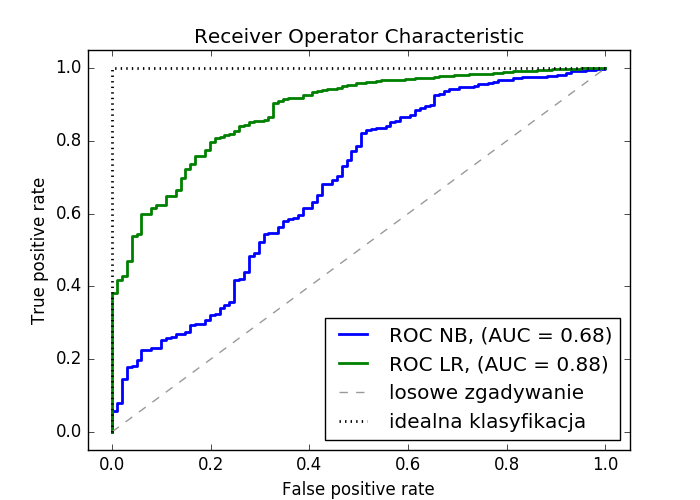
\includegraphics[width=0.6\textwidth]{./images/roc.png}
	\caption{Przykład krzywej ROC, dla naiwnego klasyfikatora bayesowskiego oraz dla regresji logistycznej dla danych "abalone0\_4\_16\_29}
	\label{fig:krzywa_roc}
\end{figure}

\todo{inline} napisac gdzies o nadmiernym dopasowaniu -> walidacja krzyżowa
\subsection{Metody pomiaru jakości klasyfikacji danych}
W celu oceny klasyfikatora powinno wykorzystywać się dwa zbiory, treningowy oraz testowy. Najpierw należy zbudować model w oparciu o dane testowe, a następnie wykonać klasyfikację testową w oparciu o zbiór testowy. W celu poprawnej oceny klasyfikacji zbioru testowego konieczna jest znajomość odpowiedniej przynależności jego składników do klas oraz zestawienie jej z przyporządkowaniem składników do klas, które zostały zasugerowane przez klasyfikator. Następnie buduje się macierz pomyłek w o parciu o sklasyfikowane przypadki. Kolejnym krokiem jest obliczenie opisanych wyżej współczynników w oparciu o tą macierz. Istnieją różne schematy postępowania, służące do oceny zbudowanego modelu.
\todo{inline} może cos napisac jeszcze o celu \url{https://en.wikipedia.org/wiki/Cross-validation_(statistics)} 
\subsubsection{Metoda z jednym zbiorem}
Do budowy klasyfikatora wykorzystywany jest cały zbiór dostępnych danych. W procesie testowania, bierze udział także cały zbiór danych. Metoda ta, nie jest zbyt wartościowa i prowadzi do zawyżenia jakości klasyfikatora. W przypadku nowych danych, taki model osiągnie gorsze wyniki niż wskazywałyby na to obliczone współczynniki.
\subsubsection{Metoda z wydzielonym zbiorem testowym (ang. \textit{the holdout method})}
W tej metodzie, zbiór danych dzielony jest w sposób losowy na dwie części. Użytkownik dobiera rozmiar zbioru uczącego (np. 80\%) oraz zbioru testowego (np. 20\%). Wadą jest, że nie wiadomo ile obiektów danej klasy znajdzie się w zbiorze testowym oraz, że zostaje zmniejszony zbiór uczący . Może to doprowadzić do sytuacji nadmiernego dopasowania (zawyżonych wyników) lub do niedoszacowania klasyfikatora. Ważne jest, aby nie używać ciągle tego samego zbioru testowego do wyboru modeli, ale dokonywać losowania przed każdą oceną.\\
Ulepszeniem tej metody, może być równy rozkład klas w obu zbiorach, tak aby zostały zachowane proporcje z oryginalnego zbioru.
\subsubsection{Sprawdzian krzyżowy z p przykładami (ang. \textit{leave-p-out cross-validation})}
Sprawdzian krzyżowy z p przykładami wykorzystuje p obserwacji jako zbiór testowy, pozostałe elementy tworzą zbiór uczący. Cały proces jest powtarzany do momentu stworzenia i przetestowania wszystkich możliwych kombinacji p przykładów ze zbioru n. Ten rodzaj metody wymaga uczenia i testowania klasyfikatora $\binom{n}{p}$ razy, gdzie n to liczebność całego zbioru danych. W przypadku dużego zbioru danych oraz p>1, obliczenia mogą zająć bardzo dużo czasu, a nawet ze względu na duża ilość kombinacji, obliczenie ich może być niemożliwe.
\subsubsection{Sprawdzian krzyżowy minus jeden element (ang. \textit{leave-one-out cross-validation})}
Jest to specjalny przypadek sprawdzaniu krzyżowego z p przykładami, dla p = 1. W tej metodzie zbiór testowy tworzy jeden element, pozostałe tworzą zbiór uczący. Testowania klasyfikatora trwa do momentu użycia wszystkich obserwacji jako zbioru testowego. W przeciwieństwie do poprzedniej metody, ta jest wolna od czasochłonnych obliczeń, gdyż $\binom{n}{1}$=n, gdzie n to liczba wszystkich obserwacji. Zazwyczaj ta metoda wykorzystywana jest tylko do małych zbiorów danych.


\subsubsection{Sprawdzian krzyżowy k-krotny (ang. \textit{k-fold cross-validation})}
Zbiór danych jest losowo dzielony na k równych podzbiorów. Następnie każdy z podzbiorów w kolejnych k iteracjach staje się kolejno zbiorem testowym, pozostałe zbiory tworzą zbiór uczący, na podstawie, którego buduje się model. Klasyfikacja i testowanie wykonywane są k-krotnie. Otrzymane wyniki łączy się i uśrednia w celu uzyskania jednego wyniku. Zaletą tej metody jest mały błąd estymacji oraz niższa wariancja błędu niż w przypadku metody minus jednego elementu. Zwykle stosuje się k=3..10, dla których koszt czasowy jest umiarkowany.
\begin{figure}[h]
	\centering
	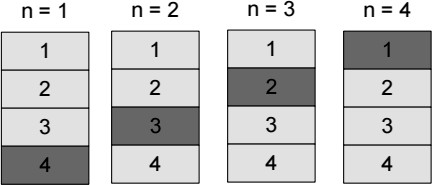
\includegraphics[width=0.6\textwidth]{./images/crossvalidation.jpg}
	\caption{Przykład sprawdzianu krzyżowego k-krotnego, k=4.}
	\label{fig:sprawdziankrzyzowy}
\end{figure}

\subsubsection{Równomierny sprawdzian krzyżowy k-krotny (ang. \textit{Stratified k-fold cross-validation})}
Jest to specjalny przypadek sprawdzianu krzyżowego k-krotnego. Podzbiory tworzone są z zachowaniem proporcji wszystkich klas. Każdy podzbiór powinien zawierać w przybliżeniu podobny procent obserwacji z każdej kategorii.

\section{Sprawdzian krzyżowy, a obliczanie miar}
W większości publikacji naukowych dotyczących klasyfikacji, jakość mierzona jest przedstawionymi wcześniej współczynnikami. 
\section{Sprawdzian krzyżowy, a oversampling}


\todo{napisac o tym, że niektóre zbiory są multiklasowe, natomiast dane sprowadzone są do 2 klas} 
\todo{napisac o podejsci one vs all}
\todo{opisac metody klasyfikacji danych mniejszosciowych, preprocessing, algorytmy}
\todo{wspomnieć o 2 podejścia -> preprecesing oraz algorytmy (algorytmamie się nie zajmuje)}
\section{!!preprocessing danych niezrównoważonych}
W celu zrównoważenia rozkładu danych niezbilansowanych wprowadzono różne metody usuwania przykładów klasy dominującej lub tworzenia sztucznych obserwacji klasy mniejszościowej. Poniżej zostaną omówione metody, które zostały użyte podczas badań.
\subsection{Metody undersampling}
Jest to cała rodzina różnych metod, które usuwają przykłady z klasy większościowej. \textbf{Losowe usuwanie} (ang. \textit{random undersampling}), jak sama nazwa wskazuje losowo usuwa przykłady z klasy dominującej. Rozwiązanie to ma niestety wadę. Jeśli usunie się zbyt dużo przykładów danego przypadku, można pozbawić klasyfikator bardzo ważnej informacji. \par
Lepszym rozwiązaniem jest świadome usuwanie przykładów spełniających określone kryteria. Taką metodą jest \textbf{undersampling z "Tomek links"}. Parę punktów Tomek link, definiuje się jako dwa punkty należące do różnych klas, z odległością równą $d(E_i,E_j)$, jeśli nie istnieje inny punkt $E_l$, taki, że $d(E_i,E_l) < d(E_i,E_j)$ lub $d(E_j,E_l) < d(E_i,E_j)$. Punkty tworzące Tomek link to szum lub punkt graniczny. Po znalezieniu takich punktów, usuwa się przykład z klasy dominującej. Usunięcie takiej obserwacji, powoduje rozszerzenie granicy klasy mniejszościowej. \par
\todo{opisac reszte te ktore wykorzystam}

\subsection{Metody oversampling}




\chapter{Klasyfikacja danych niezrównoważonych}
Większość istniejących algorytmów klasyfikacji, nastawiona jest na poprawną klasyfikację zbiorów o~zrównoważonej liczebności wszystkich klas. Niestety, w~rzeczywistych problemach, bardzo często zdarza się, że zbiory są mocno niezbilansowane. Istnieją dwie metody pozwalające zwiększyć skuteczność klasyfikacji danych mniejszościowych. W pierwszej metodzie modyfikuje się dane treningowe przed procesem uczenia. Dodaje się lub usuwa przykłady w~celu zrównoważenia liczebnie obu klasy. W drugim podejściu wykorzystuje się zmodyfikowane algorytmy pod kątem niezrównoważonych zbiorów. W niniejszej pracy skupiono się wyłącznie na pierwszej metodzie, równoważeniu zbiorów.	
\section{Dane niezrównoważone}
Dane są niezrównoważone (ang. \textit{imbalanced data}) jeśli klasy decyzyjne nie są w~przybliżeniu tak samo liczebne. Najmniejsza klasa nazywana jest klasą mniejszościową (ang. \textit{minority class}), natomiast klasa dominująca, lub pozostałe połączone klasy (można połączyć pozostałe klasy w~jedną, doprowadzając do klasyfikacji binarnej, one vs all), nazywana jest klasą większościową (ang. \textit{majority class}). W praktyce klasa mniejszościowa zazwyczaj liczy około 10-20\% wszystkich przykładów. Często zdarzają się jednak takie problemy, gdzie to zróżnicowanie jest większe np.:
\begin{itemize}
	\item około 2\% transakcji kartami kredytowymi w~GOCARDLESS to oszustwa \cite{gocardless},
	\item dane medyczne zawierają bardzo dużą liczbę zdrowych pacjentów, a~liczba chorych to najczęściej kilka procent lub mniej,
	\item około 1\% rocznie twardych dysków ulega awarii.
	
\end{itemize}

W przytoczonych przykładach ważniejsza jest klasa mniejszościowa i~wykrycie jej stanowi priorytet. Niezrównoważenie klas w zbiorze danych stanowi problem w fazie uczenia i znacząco obniża jakość klasyfikacji. Ze względu na częstość występowania klasy dominującej, klasyfikator preferuje tą klasę, dążąc do optymalizacji i~obniżenia błędu error rate (rozdział \ref{error_rate}) nie biorąc pod uwagę rozłożenia klas w~zbiorze. Klasyfikator może osiągnąć wysoką skuteczność klasyfikacji np. 95\%, przy niskiej lub zerowej wykrywalności klasy mniejszościowej. 
Należy oczekiwać od klasyfikatora wysokiej skuteczności wykrywania klasy mniejszościowej, nawet kosztem pogorszenia rozpoznawania klasy większościowej.
Przykłady z~klasy zdominowanej można podzielić na cztery grupy. K. Napierała i~J. Stefanowski wyróżnili przykłady\cite{przykladyklas}:
\begin{itemize}
	\item safe - przykład bezpieczny, w~jego sąsiedztwie zdecydowana większość obserwacji jest z~tej samej klasy,
	\item borderline - graniczny, przykład niebezpieczny, w~jego sąsiedztwie liczba przykładów z~obu klas jest podobna
	\item outlier - poboczny, przykład niebezpieczny, w~jego sąsiedztwie większość obserwacji jest z~klasy przeciwnej, dominującej,
	\item rare - rzadki, przykład niebezpieczny, w~jego sąsiedztwie występują tylko przykłady z~klasy przeciwnej, większościowej.
\end{itemize}

\section{Równoważenie rozkładu klas w~zbiorze danych}
\label{rozdzialopissamplingu}
W celu zrównoważenia rozkładu danych niezbilansowanych wprowadzono różne metody usuwania przykładów klasy dominującej lub tworzenia sztucznych obserwacji klasy mniejszościowej. Poniżej zostaną omówione metody, które zostały użyte podczas badań.
\subsection{Metody undersampling}
Jest to cała rodzina różnych metod, które usuwają przykłady z~klasy większościowej. \textbf{Losowe usuwanie} (ang. \textit{random undersampling}), jak sama nazwa wskazuje, usuwa losowo przykłady z~klasy dominującej. Rozwiązanie to ma niestety wadę. Jeśli usunie się zbyt dużo przykładów danego przypadku, można pozbawić klasyfikator bardzo ważnej informacji. \par
Lepszym rozwiązaniem jest świadome usuwanie przykładów spełniających określone kryteria. Taką metodą jest \textbf{undersampling z~,,Tomek links''} \cite{tomelinksc}. Parę punktów Tomek link, definiuje się jako dwa punkty należące do różnych klas, z~odległością równą $d(E_i,E_j)$, jeśli nie istnieje inny punkt $E_l$, taki, że $d(E_i,E_l) < d(E_i,E_j)$ lub $d(E_j,E_l) < d(E_i,E_j)$. Punkty tworzące Tomek link to szum lub punkt graniczny. Po znalezieniu takich punktów, usuwa się przykład z~klasy dominującej. Usunięcie takiej obserwacji powoduje rozszerzenie granicy klasy mniejszościowej. \par
W metodzie \textbf{\textit{Edited Nearest Neighbour}} (ENN) \cite{enn} analizowane są przykłady klasy większościowej. Usuwany jest każdy niewiarygodny przykład, jeżeli z~trzech sąsiadów, przynajmniej dwóch ma inną klasę. \par
Modyfikacją metody ENN jest bardziej rygorystyczna reguła \textbf{\textit{Neighbour Cleaning Rule}} (NCR) \cite{ncr}. Usuwa ona zdecydowanie więcej przykładów z~klasy większościowej. Usuwany jest każdy przykład dominującej klasy, jeżeli w~jego sąsiedztwie znajdują się przynajmniej dwie obserwacje z~klasy mniejszościowej. Dodatkowo, jeżeli w~otoczeniu przykładu klasy zdominowanej znajdują się dwa przykłady z~klasy dominującej, to te dwa przykłady również są usuwane.

\subsection{Metody oversampling}
Metody z~rodziny oversampling generują nowe sztuczne obserwacje klasy mniejszościowej. Najprostszą metodą tworzenia nowych przykładów jest \textbf{losowe próbkowanie} (ang. \textit{random oversampling}). Polega ona na kopiowaniu losowo wybranych przykładów z~klasy mniejszościowej. Metoda ta, może doprowadzić do nadmiernego dopasowania, szczególnie w~przypadku wielokrotnego skopiowania przykładów stanowiących szum. \par
Lepszym wyborem niż losowe tworzenie próbek może być metoda \textbf{\textit{SMOTE}} (\textit{Synthetic Minority Over-sampling Technique}) \cite{smotec}, która generuje nowe sztuczne obserwacje. W metodzie tej, analizowanych jest $k$ najbliższych sąsiadów obserwacji z~klasy mniejszościowej. Następnie generowane są nowe sztuczne przykłady, na losowo wybranych punktach z~odcinków łączących analizowany przykład z~sąsiadami. Liczbę wygenerowanych próbek można zdefiniować, w~zależności od potrzebnej liczby nowych obserwacji. SMOTE nie analizuje przykładów z~drugiej klasy, co może prowadzić do większego wymieszania obu klas, a~w konsekwencji do pogorszenia skuteczności klasyfikacji. \par
Rozwinięciem metody SMOTE jest algorytm \textbf{\textit{ADASYN}} (\textit{Adaptive Synthetic Sampling Approach for Imbalanced Learning}) \cite{adasync}. Metoda ADASYN podobnie jak SMOTE, generuje nowe sztuczne obserwacje klasy mniejszościowej, jednak skupia się bardziej na przykładach trudniejszych w~klasyfikacji. Algorytm SMOTE generuje taką samą liczbę nowych próbek dla każdego przykładu klasy zdominowanej. ADASYN wprowadza różne wagi dla obserwacji klasy mniejszościowej, dzięki czemu można skuteczniej klasyfikować trudniejsze przykłady.
\subsection{Metody hybrydowe}
W celu zrównoważeniu zbioru danych można połączyć metody oversampling oraz undersampling. Przykładem takich połączonych metod jest \textbf{SMOTE z~ENN} (SMOTENN) oraz \textbf{SMOTE z~Tomek links} (SMOTETOMEK) \cite{hybrid}. Tworzenie nowych próbek odbywa się tak jak metodzie SMOTE, a~następnie usuwane są przykłady klasy większościowej według wybranego algorytmu (ENN lub Tomek links). Dodatkowo usuwane są sztuczne wygenerowane obserwacje, które za bardzo ingerują w~przestrzeń klasy większościowej.

\chapter{Przeprowadzone badania}
\section{Projekt klasyfikatora}
\subsection{Klasyfikator ekspercki}
Klasyfikator ekspercki powstał na bazie doświadczeń z podstawowymi klasyfikatorami. W zależności o charakterystyki danych, osiągana skuteczność przez klasyfikatory może się różnić. Klasyfikator skutecznie rozpoznający klasy jednego zbioru, może miernie klasyfikować inny zbiór, podczas gdy użycie innego klasyfikatora na tym samym zbiorze danych może znacząco poprawić osiągane wyniki. Również użycie różnych algorytmów klasyfikacji, połączenie ich w komitet może zmniejszyć błąd klasyfikacji. 
Klasyfikator ekspercki został stworzony w celu zmniejszenia błędu klasyfikacji niezależnie od typu danych oraz nieznanych danych. \par
\begin{figure}[h]
	\centering
	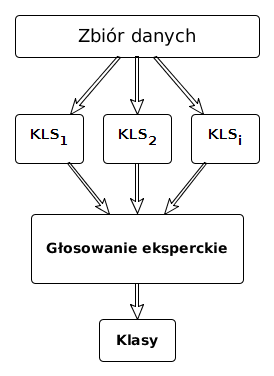
\includegraphics[width=\textwidth]{./images/klas_ekspercki.png}
	\caption{Schemat klasyfikatora eksperckiego. $KB_1..KB_i$ to klasyfikatory bazowe.}
	\label{fig:klasyfikator_ekspercki}
\end{figure}
Klasyfikator ekspercki to połączenie kilku klasyfikatorów bazowych (przynajmniej trzech). Każdy klasyfikator trenowany jest na zbiorze uczącym, a następnie oceniana jest jakość klasyfikacji każdego z osobna. Stworzono dwie wersje klasyfikatora, w pierwszej klasyfikator uczony i testowany jest na tym samym zbiorze danych, w drugiej oceniany jest z wykorzystaniem sprawdzianu krzyżowego (domyślnie k=3). W kolejnym etapie, dla każdej klasy wyłaniany jest klasyfikator ekspert. Ekspert klasowy wybierany jest na podstawie najwyższego współczynnika dla danej klasy. Tworząc klasyfikator można wybrać na podstawie którego współczynnika precyzji, F1 czy G-mean będą wyłaniani eksperci. Domyślnie jest to współczynnik precyzji. Przy wyborze miary G-mean ekspert dla obu będzie taki sam. Jeżeli ocena odbywała się ze sprawdzianem krzyżowym, to modele bazowe tworzone są od nowa na całym zbiorze treningowym. \par
W procesie klasyfikacji właściwej nowych próbek, najpierw klasyfikowane są przez klasyfikatory bazowe. Końcowa klasa wyznaczana jest według algorytmu:
\begin{enumerate}
	\item Jeżeli występuje zgodność co do klasy pomiędzy klasyfikatorami to wybierana jest ta klasa.
	\item Jeżeli tylko jeden ekspert wskaże swoją klasę to ostateczną klasą jest ta wskazana przez eksperta.
	\item Jeżeli dwóch ekspertów wskażą swoje klasy, to wybierana jest klasa z większym prawdopodobieństwem wskazanym przez klasyfikator. W przypadku takich samych prawdopodobieństw, wybierana jest klasa wskazana przez klasyfikator z większym współczynnikiem G-mean.
	\item Jeżeli żaden ekspert nie wskaże swojej klasy, to klasa wybierana jest poprzez głosowanie większościowe
\end{enumerate}

\subsection{Meta-klasyfikator}
\section{Opis platformy i w jaki sposób zrealizowano badania}

\subsection{Język python}
Wszystkie badania i testy zostały napisane z wykorzystaniem języka python. Jest to język programowania interpretowany, wysokiego poziomu z dużą ilością dostępnych bibliotek. Python\cite{python} posiada dynamiczne zarządzanie typami oraz automatyczne zarządzanie pamięcią. Wspiera kilka paradygmatów programowania, takich jak: obiektowy, imperatywny, funkcyjny i proceduralny. Został zaprojektowany z myślą o czytelności kodu oraz składnią pozwalającą napisać program z mniejszą ilością kodu niż w językach C++ lub Java. Implementacja języka python dostępna jest na wiele systemów operacyjnych. Często wykorzystywany jest jako język skryptowy. Python jest projektem typu Open Source. \par
W pracy wykorzystano język python w wersji 2.7.11. Język ten wybrano ze względu na łatwość pisania w nim kodu, szybką możliwość nauki oraz na szeroki wachlarz dostępnych bibliotek. Ważnym argumentem w wyborze były gotowe biblioteki z klasyfikatorami oraz do pracy z klasyfikacją danych. Dostępność bibliotek do wizualizacji dla tego języka, pozwoliła na przedstawienie wyników testów w formie graficznej. Napisane testy można w łatwy sposób rozbudować, zmodyfikować lub dodać nowe elementy.    

\subsection{Biblioteka scikit-learn}
Scikit-learn\cite{scikit} to proste i wydajne narzędzie do analizy i eksploracji danych. Jest to biblioteka uczenia maszynowego dla języka python. Rozpowszechnianie oparta jest na licencji BSD. W Scikt-learn zaimplementowane są (lub napisany jest kod obsługujący) różne algorytmy klasyfikacji, regresji, analizy skupień takie jak: maszyna wektorów nośnych, algorytmy najbliższego sąsiada, naiwny Bayes, drzewa decyzyjne, sieć neuronowa, zespoły klasyfikatorów. Z wykorzystaniem tej biblioteki można przygotować oraz przetworzyć odpowiednio dane. Możliwe jest także, ocenianie oraz wizualizacja wyników. \par
W testach użyto biblioteki scikit-learn w wersji 0.18.1. Wykorzystano z niej algorytmy klasyfikacji oraz wstępnego przetwarzania danych.
\subsection{Biblioteka imbalanced-learn}
Biblioteka imbalanced-learn\cite{imlearn} zawiera zestaw narzędzi do wstępnego przetwarzania danych niezrównoważonych. Posiada ona zaimplementowane różne metody under- oraz over-sampling do równoważenia zbiorów danych. W pracy wykorzystano te metody z biblioteki w wersji 0.2.1. 
\subsection{Pozostałe użyte biblioteki}
\subsubsection{Mlxtend}
Mlxtend (machine learning extensions)\cite{mlxtend} jest to biblioteka zawierająca różne narzędzia do pracy z danymi. W badaniach wykorzystano z niej algorytm Stacking.
\subsubsection{Numpy}
Numpy to pakiet umożliwiający obliczenia naukowe. Szczególnym elementem jest możliwość wykonywania obliczeń na tablicach N-wymiarowych. 
\subsubsection{Maptolib}
Maptolib to biblioteka pythona, która tworzy różnego rodzaju wykresy 2D oraz interaktywne na różnych platformach.
\subsubsection{Texttable}
Texttable to prosty moduł napisany w języku python, służący do produkcji prostych tabel ASCII. Został wykorzystany do prezentacji wyników w konsoli.
\subsubsection{Pylatex}
Pylatex to biblioteka pythona, służąca do tworzenia i kompilacji plików LaTeX. W pracy została wykorzystana do zapisu wyników w badań w plikach .tex oraz .pdf.
\subsection{opisac co zaimplementowane?}
\todo{ze wlasna krosswalidacja, ze wlasne miary, klasyfikator. itd}

\todo{inline} napisac o roznych F i o tym jak wyniki wyglada, pokazać test

\section{Opis danych użytych w badaniach}
Do przeprowadzenia badań użyto 26 różnych prawdziwych zbiorów danych (tabela \ref{danebadania}) pochodzących z repozytorium serwisu "The UCI Machine Learning Repository" \cite{uci}. Dane wybrano ze względu na różnorodność typów danych, ilości rekordów, atrybutów oraz zróżnicowanie rozkładu klas. Większość z danych była używana w publikacjach podobnych tematycznie\cite{hyper}\cite{StefImbalanced}. \par
Wszystkie dane zostały zapisane w skrypcie, w folderze $praca/data/files$, a opis szczegółowy danych znajduje się w folderze $praca/data/files/data\_descrytpion$. Do importu danych służą funkcje z pliku $praca/data/import\_data.py$. Do ogólnego importu danych z pliku, służy funkcja $importfile$, zaś wczytywanie danych użytych w projekcie odbywa się poprzez funkcje zaczynające się od $load\_$. Import danych z pliku odbywa się z wykorzystaniem funkcji z pakietu $numpy$ $genfromtext$ oraz $load\_txt$. Atrybuty posiadające dane kategoryczne zapisane w postaci łańcuchów znaków zostały zamienione na dane numeryczne. Cechy nominalne zostały zakodowane metodą $one hot encoding$. Dla danych zawierających więcej niż dwie klasy, klasa z najmniejszą liczebnością została wybrana jako klasa mniejszościowa, pozostałe klasy utworzyły klasę większościową. We wszystkich zbiorach danych, kategorie reprezentowane są w systemie binarnym. Pięć zbiorów danych posiadało brakujące wartości. Zostały one zastąpione wartościami środkowymi zbioru (medianą).
\begin{table}[H]
	\begin{center}
		\resizebox{\textwidth}{!}{%
			\begin{tabular}{|c|c|c|c|c|c|}%
				\hline%
				Nazwa danych&L. el.&Atrybuty&Rozkład klas&\% kl. mn.&IR\\%
				\hline%
				abalone0\_4&4177&8&4103/74&1.77&55.45\\%
				abalone041629&4177&8&3842/335&8.02&11.47\\%
				abalone16\_29&4177&8&3916/261&6.25&15.0\\%
				balance\_scale&625&4&576/49&7.84&11.76\\%
				breast\_cancer&286&9&201/85&29.72&2.36\\%
				bupa&341&6&200/141&41.35&1.42\\%
				car&1728&6&1663/65&3.76&25.58\\%
				cmc&1473&9&1140/333&22.61&3.42\\%
				ecoli&336&7&301/35&10.42&8.6\\%
				german&1000&24&700/300&30.0&2.33\\%
				glass&214&9&197/17&7.94&11.59\\%
				haberman&306&3&225/81&26.47&2.78\\%
				heart\_cleveland&303&13&268/35&11.55&7.66\\%
				hepatitis&155&19&123/32&20.65&3.84\\%
				horse\_colic&368&22&232/136&36.96&1.71\\%
				ionosphere&351&34&225/126&35.9&1.79\\%
				new\_thyroid&215&5&185/30&13.95&6.17\\%
				postoperative&90&8&66/24&26.67&2.75\\%
				seeds&210&7&140/70&33.33&2.0\\%
				solar\_flare&1066&10&1023/43&4.03&23.79\\%
				transfusion&748&4&569/179&23.93&3.18\\%
				vehicle&846&18&647/199&23.52&3.25\\%
				vertebal&310&6&210/100&32.26&2.1\\%
				yeastME1&1484&8&1440/44&2.96&32.73\\%
				yeastME2&1484&8&1433/51&3.44&28.1\\%
				yeastME3&1484&8&1321/163&10.98&8.1\\%
				\hline%
			\end{tabular}}
			\caption{Dane użyte w badaniach wraz z charakterystyką.}
			\label{danebadania}
		\end{center}
	\end{table}
\subsubsection{Analiza klas mniejszościowych}
Dane użyte w badaniach poddano analizie sąsiedztwa w celu określenia przynależności przykładów z klasy mniejszościowej do jednej z czterech grup. Analizę wykonano z wykorzystaniem algorytmu k najbliższych sąsiadów, k = 5. Do pomiaru odległości wykorzystano miarę Czebyszewa. Skrypt analizujący dane znajduje się w pliku: $analyze\_db.py$ Przykłady klasyfikowano do grup w zależności od ilości sąsiadów\cite{przykladyklas}:
\begin{itemize}
	\item safe - jeżeli w sąsiedztwie znajdowało się przynajmniej 4 przykłady z tej samej klasy,
	\item border - jeżeli liczba przykładów z obu klas była podobna, tj. dla 2-3 przykłady z tej samej klasy,
	\item rare - jeżeli w sąsiedztwie był tylko jeden przykład z tej klasy,
	\item outlier - jeżeli wszyscy sąsiedzi należeli do innej klasy.
\end{itemize}
Wyniki analizy przedstawiono w tabeli \ref{dane_analiza_grupy}.
\begin{table}[h]
	\scriptsize
	\begin{center}
		\resizebox{\textwidth}{!}{%
			\begin{tabular}{c|cccc}%
				&Safe [\%]&Borderline [\%]&Rare [\%]&Outlier [\%]\\%
				\hline%
				seeds&88.57&10.0&0.0&1.43\\%
				new\_thyroid&73.33&10.0&6.67&10.0\\%
				vehicle&62.81&26.63&2.51&8.04\\%
				ionosphere&57.94&21.43&13.49&7.14\\%
				vertebal&56.0&33.0&2.0&9.0\\%
				yeastME3&50.92&32.52&10.43&6.13\\%
				yeastME1&36.36&52.27&0.0&11.36\\%
				ecoli&31.43&48.57&14.29&5.71\\%
				bupa&27.66&48.23&8.51&15.6\\%
				horse\_colic&22.79&52.94&13.24&11.03\\%
				abalone0\_4&37.84&32.43&18.92&10.81\\%
				german&9.0&51.33&14.67&25.0\\%
				breast\_cancer&3.53&52.94&12.94&30.59\\%
				cmc&12.31&43.24&20.42&24.02\\%
				hepatitis&0.0&53.12&15.62&31.25\\%
				haberman&12.35&38.27&18.52&30.86\\%
				yeastME2&3.92&35.29&35.29&25.49\\%
				abalone041629&11.04&31.94&30.75&26.27\\%
				transfusion&13.41&36.31&21.79&28.49\\%
				car&1.54&33.85&35.38&29.23\\%
				glass&0.0&47.06&23.53&29.41\\%
				abalone16\_29&3.45&31.8&34.1&30.65\\%
				solar\_flare&4.65&16.28&46.51&32.56\\%
				heart\_cleveland&0.0&5.71&48.57&45.71\\%
				balance\_scale&0.0&22.45&30.61&46.94\\%
				postoperative&0.0&33.33&8.33&58.33\\%
			\end{tabular}}
			\caption{Analiza przynależności przykładów z klasy mniejszościowej do grup. Dane posortowano w kolejności od najłatwiejszych w klasyfikacji do najtrudniejszych.}
			\label{dane_analiza_grupy}
		\end{center}
	\end{table}

\todo{opisac foldy w zaleznosci od ilosci danych}
\section{Sposób mierzenia w sprawdzianie krzyżowym}
\section{Ocena klasyfikatora w sprawdzianie krzyżowym k-krotnym.}
W większości publikacji naukowych dotyczących klasyfikacji, ocena klasyfikatora mierzona jest z wykorzystaniem sprawdzianu krzyżowego (zwykle k=10) oraz przedstawionych wcześniej miar. Jednakże, w tych publikacjach nie został opisany sposób obliczania współczynników w czasie sprawdzianu krzyżowego. Wykorzystanie różnych sposobów prowadzi do różnych wyników. Niektóre metody są mniej lub bardziej obciążone błędem. Różnice w wynikach, wynikające z przyjętej metody obliczeniowej, są szczególnie widoczne w sprawdzianie krzyżowym z losowym rozkładem danych oraz w klasyfikacji danych niezrównoważonych. Są dwie główne możliwości obliczania współczynników:
\begin{itemize}
	\item obliczanie wartości współczynników dla każdej k-iteracji (klasyfikatora), a następnie obliczenie średniej z tych iteracji,
	\item stworzenie jednej wspólnej macierzy pomyłek dla każdej k-iteracji, a następnie obliczenie wskaźników.
\end{itemize}
W przypadku drugiego sposobu, poszczególne elementy macierzy pomyłek będą wynosić odpowiednio:
\[TP := \sum_{i=1}^{k} TP^{(i)}\]
\[FP := \sum_{i=1}^{k} FP^{(i)}\]
\[TN := \sum_{i=1}^{k} TN^{(i)}\]
\[FN := \sum_{i=1}^{k} FN^{(i)}\]
\subsection{Test sposobów oceny klasyfikatora}
W celu wyboru najlepszego sposobu oceny klasyfikatora, z najmniejszym błędem oraz wariancją wykonano pięć porównujących testów dla różnych metod obliczania miar. Wszystkie testy miały takie same założenia oraz sposób wykonania. Testy wykonano na wygenerowanych losowo danych dla różnej ilości przykładów pozytywnych (od 1\% do 10\%). Jakość klasyfikacji była oceniana dla równomiernego sprawdzianu krzyżowego oraz dla losowego. Symulacje odbyły się one w następujący sposób:

\begin{enumerate}
	\item Wygeneruj zbiór 1500 losowych próbek z 2 atrybutami, 2 klasami o rozkładzie 4:1.
	\item Wykonaj niezrównoważenie zbioru z ratio 0.1
	\item Wybierz m=[1..10]*10 przykładów klasy mniejszościowej oraz 1000-m przykładów klasy dominującej.
	\begin{enumerate}
		\item  Wykonaj N iteracji:
		\begin{enumerate}
			\item Wymieszaj dane.
			\item Wykonaj sprawdzian krzyżowy k-krotny, k=10.
			\item Oblicz współczynniki dla obu metod.
		\end{enumerate}
		\item Oblicz odchylenie standardowe oraz średnie wartości współczynników.
	\end{enumerate}
	\item Przedstaw wyniki odchylenia standardowego oraz średnie wartości współczynników dla różnego rozkładu klas.
\end{enumerate}
Wykonanie testu N-krotnie (najlepiej n>100000) pozwala na obliczenie "prawdziwych" wartości miar oceny klasyfikacji. Powtórzenie sprawdzianu krzyżowego wielokrotnie pozwala na ocenę błędu oraz wariancji miar dla każdej metodyki. Przeprowadzenie testu dla danych zawierających tylko 1\% obserwacji klasy mniejszościowej (przypadek ekstremalny, w zbiorze danych znajduje się wtedy tylko 10 takich przykładów) oznacza, że w niektórych iteracjach sprawdzianu krzyżowego nie będzie przykładów poprawnie sklasyfikowanych z tej klasy. Brak dobrze sklasyfikowanych przykładów klasy mniejszościowej może mieć także miejsce w losowym sprawdzianie krzyżowym. Wynika to z braku równomiernego rozkładu obu klas. 
\subsubsection{Dokładność oraz błąd klasyfikatora}
Dokładność klasyfikacji oraz błąd klasyfikatora, korzystając z metody pierwszej, będzie wynosić:
\[accuracy_{avg} := \frac{1}{k} \sum_{i=1}^{k} accuracy^{(i)}\]
a błąd klasyfikatora:
\[error\ rate_{avg} = 1 - accuracy_{avg}\]
Obliczając drugim sposobem, korzysta się z podstawowego wzoru z wykorzystaniem wspólnej macierzy pomyłek. \par
W przypadku dokładności oraz błędu klasyfikatora, niezależnie od przyjętej metodyki otrzymane wartości będą takie same, nieobciążone błędem.
\subsubsection{Czułość, specyficzność, FPR oraz precyzja}
Czułość, specyficzność, FPR oraz precyzja w metodzie pierwszej oblicza się wg. wzorów:
\[Sensitivity_{avg},\ Recall_{avg},\ TPR_{avg} := \sum_{i=1}^{k} TPR_{avg}^{(i)}\]
\[Specificity_{avg},\ TNR_{avg} := \sum_{i=1}^{k} TNR_{avg}^{(i)}\]
\[FPR_{avg} := \sum_{i=1}^{k} FPR_{avg}^{(i)}\]
\[Precision_{avg} := \sum_{i=1}^{k} Precision_{avg}^{(i)}\]
W drugim sposobie korzysta się z wspólnej macierzy pomyłek oraz z podstawowych wzorów. \par
Testy wyżej wymienionych współczynników, zostały przeprowadzone z wykorzystaniem skryptu $test\_wsk.py$. Zauważono, że w przypadku równomiernego sprawdzianu krzyżowego, różnica w wynikach jest bardzo mała, poniżej 0.5\%. Obie metody obarczone sa małym błędem i wariancją. Natomiast w przypadku sprawdzianu krzyżowego z rozkładem losowym, metoda druga okazała się lepsza. Obliczona czułość oraz precyzja sposobem drugim, uzyskały wyniki z mniejszym błędem, bliższe wartości "prawdziwej". Natomiast specyficzność w obu metodach wyszła taka sama, ze względu na dużą liczbę przykładów z tej klasy. Sprawdzone, że w momencie odwrócenia liczebności klas, specyficzność posiada taką samą charakterystykę jak czułość. Różnice w wynikach obu sposobów zmniejszają się wraz ze wzrostem przykładów klasy większościowej. Zazwyczaj przy 10\% zawartości danych klasy zdominowanej w zbiorze, wyniki są takie same.
\begin{figure}[H]
	\centering
	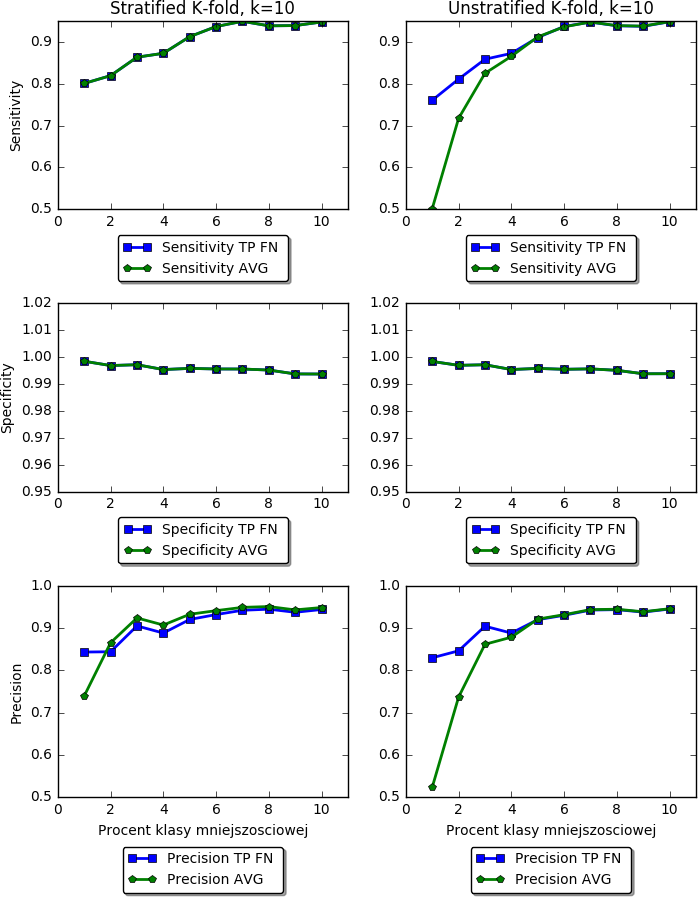
\includegraphics[width=\textwidth]{./images/wsk.png}
	\caption{Wykresy czułości, specyficzności oraz precyzji w zależności od wielkości klasy mniejszościowej dla równomiernego oraz losowego sprawdzianu krzyżowego (k=10).}
	\label{fig:wskazniki}
\end{figure}

\begin{figure}[H]
	\centering
	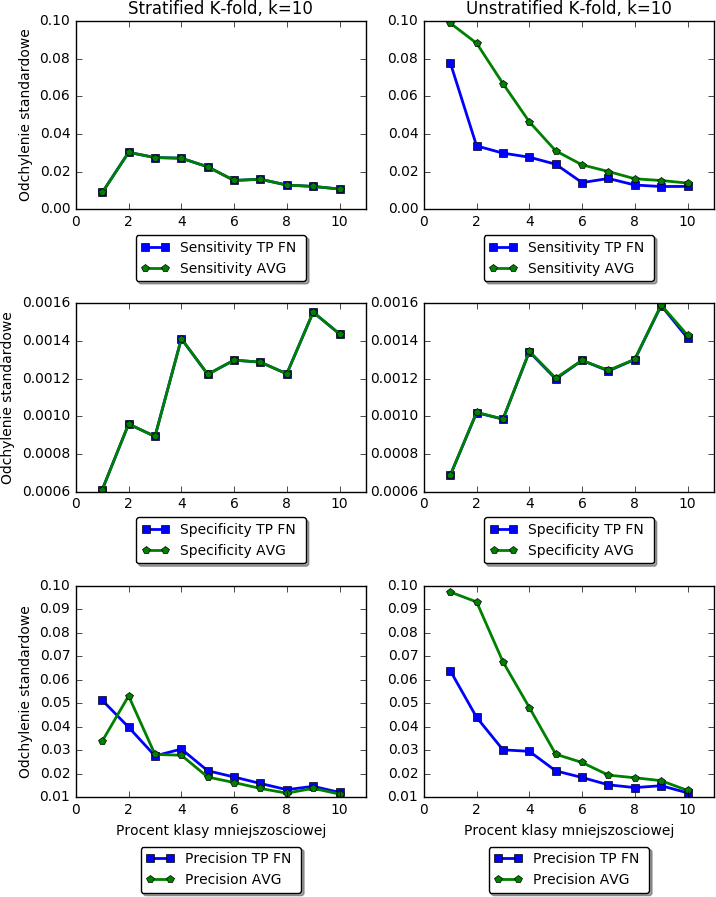
\includegraphics[width=\textwidth]{./images/stdwsk.png}
	\caption{Odchylenie standardowe miar czułości, specyficzności oraz precyzji w zależności od wielkości klasy mniejszościowej dla równomiernego oraz losowego sprawdzianu krzyżowego (k=10).}
	\label{fig:wskaznikistd}
\end{figure}
\todo{wstawic wykres i opisac}
\subsubsection{Miara $F_1$}
W niniejszej pracy oraz w wielu publikacjach miara F-measure obliczana jest dla $\beta=1$, dlatego testy przeprowadzono tylko dla tej wartości. Miarę F, można obliczyć na trzy różne sposoby. Pierwszy polega na obliczeniu F dla każdego k klasyfikatora, a następnie uśrednienie wyników:
\[F_{avg} := \frac{1}{k} \sum_{i=1}^{k} F_1^{(i)}\]
Drugi sposób, to obliczenie średniej czułości i precyzji, a następnie miary F z podstawowego wzoru:
\[Pre_{avg} := \frac{1}{k} \sum_{i=1}^{k} Pre^{(i)}\]
\[Re_{avg} := \frac{1}{k} \sum_{i=1}^{k} Re^{(i)}\]
\[F_{pre, re} = 2 * \frac{Pre_{avg}*Re_{avg}}{Pre_{avg}+Re_{avg}} \]
Ostatnio sposób, to obliczenie współczynnika F ze wspólnej, końcowej macierzy pomyłek:
\[F_{tp, fp, fn} = \frac{2*TP}{2*TP+FP+FN} \]
Do powyższych wzorów można dodać jeszcze sposób odrzucający oceny klasyfikatorów, dla których precyzja lub czułość są niezdefiniowane. Ta metoda została odrzucona ze względu na zawyżanie końcowej oceny. \par 
Skrypt testujący powyższe trzy sposoby znajduje się w pliku $test\_f1.py$. Analizując otrzymane wyniki (wykres \ref{fig:wykresf1}), zauważono, że najbardziej powtarzalne wyniki otrzymano korzystając z wzoru $F_{tp, fp, fn}$. W przypadku obu sprawdzianów krzyżowych, metoda ta generowała najmniejszy błąd. Zauważono, że niezależnie od ilości danych niezrównoważonych, otrzymane wyniki tą metodą różniły się nieznacznie, w przeciwieństwie do pozostałych sposobów. Podobnie jak w przypadku poprzednich miar, wraz ze wzrostem ilości danych niezrównoważonych, uzyskiwane wyniki były prawie takie same, niezależnie od sposobu obliczania.
\begin{figure}[H]
	\centering
	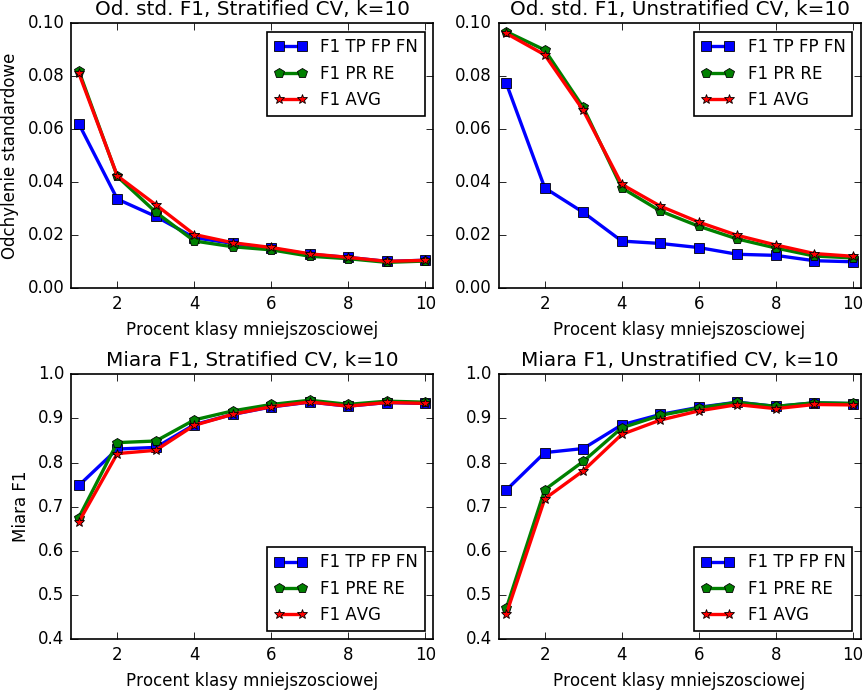
\includegraphics[width=\textwidth]{./images/miara-F1.png}
	\caption{Wykres odchylenia standardowego miar F1 oraz średniej miar F1 w zależności od wielkości klasy mniejszościowej dla równomiernego oraz losowego sprawdzianu krzyżowego (k=10).}
	\label{fig:wykresf1}
\end{figure}
\subsubsection{Miara G-mean}
Miara G-mean może zostać obliczona również na trzy różne sposoby. Pierwszy z nich to średnia z wszystkich klasyfikatorów:
\[G-mean_{avg} := \frac{1}{k} \sum_{i=1}^{k} G-mean^{(i)} \]
W drugim sposobie należy najpierw obliczyć średnią wartość czułości oraz specyficzności, a końcowy wynik G-mean oblicza się z głównego wzoru:
\[G-mean_{Se, Sp} = \sqrt{Sensitivity_{avg}*Specificity_{avg}} \]
W ostatniej metodzie obliczania G-mean, za czułość oraz specyficzność, wstawia się właściwie wzory, a wartość oblicza się na podstawie zsumowanej macierzy pomyłek.
\[G-mean_{tp, fp, fn} = \sqrt{\frac{TP}{TP + FN}*\frac{TN}{TN + FP}} \]
Skrypt testujący powyższe wzory znajduje się w pliku $test\_g\_mean.py$. Analizując wyniki (wykres \ref{fig:wykresgmean}) równomiernego sprawdzianu krzyżowego, zaobserwowano, że  wyniki $G-mean_{tp, fp, fn}$ oraz $G-mean_{Se, Sp}$ pokrywają się. Natomiast w zwykłym sprawdzianie krzyżowym, pomiarem najmniej obarczonym błędem był $G-mean_{tp, fp, fn}$. Z wykorzystaniem tego wzoru, dla różnej zawartości klasy mniejszościowej w zbiorze danych otrzymano wyniki różniące się jedynie o kilka procent pomiędzy sobą, podczas gdy wyniki pozostałych metod różniły się aż o 15\%-30\%. Jednocześnie ta metoda dawała najmniejszy błąd odchylenia standardowego. Zauważono także, że w przypadku zawartości minimum 6\% klasy mniejszościowej w danych, otrzymywane wyniki różnią się nieznacznie (poniżej 1\%).
\begin{figure}[H]
	\centering
	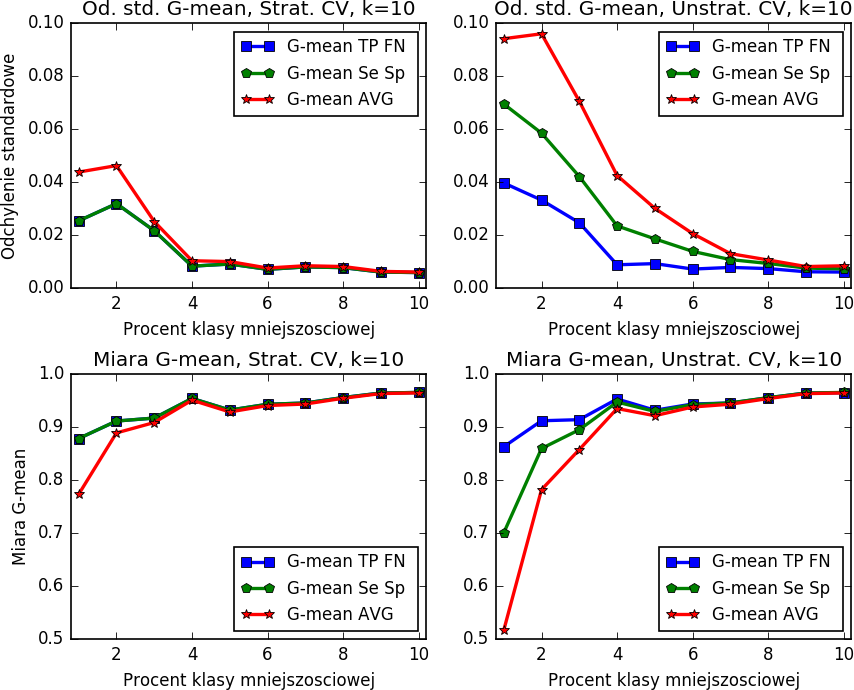
\includegraphics[width=\textwidth]{./images/miara-G-mean.png}
	\caption{Wykres odchylenia standardowego miar G-mean oraz średniej miar G-mean w zależności od wielkości klasy mniejszościowej dla równomiernego oraz losowego sprawdzianu krzyżowego (k=10).}
	\label{fig:wykresgmean}
\end{figure}
\subsubsection{Krzywa ROC i miara AUC}
Wartość AUC w sprawdzianie krzyżowym można skonstruować na dwa sposoby. W pierwszej metodzie, konstruuje się krzywą ROC oraz oblicza się AUC dla każdego k klasyfikatora. Następnie oblicza się $AUC_{AVG}$ poprzez obliczenie średniej:
\[AUC_{AVG} := \frac{1}{k} \sum_{i=1}^{k} AUC^{(i)} \]
W przypadku sprawdzianu krzyżowego z losowym rozkładem klas, może okazać się, że nie sklasyfikowano żadnego przykładu pozytywnego. Wtedy skonstruowanie krzywej ROC oraz obliczenie AUC będzie niemożliwe. W takich przypadkach podczas obliczania $AUC_{AVG}$ można pominąć taki wynik. \par
Drugim sposobem jest połączenie prawdopodobieństwa przykładów testowych z każdej iteracji. Z połączonych obserwacji, konstruuje się jedną krzywą ROC i oblicza $AUC_{merge}$. Korzystając z tego sposobu, zakłada się, że klasyfikator ma dobrze skalibrowane określanie prawdopodobieństwa.  Test obu metod zostały przeprowadzone z użyciem skryptu $test\_roc.py$ i danych $transfusion$. Wygenerowane krzywe (wykres \ref{fig:cv_roc}) ROC k klasyfikatorów różnią się od siebie kształtem oraz powierzchnią AUC. W obu sprawdzianach krzyżowych obliczona średnia $ROC_{AVG}$ oraz $AUC_{AVG}$ znajdują się pomiędzy wartościami otrzymanymi z klasyfikatorów cząstkowych (fold). Natomiast w sprawdzianie krzyżowym równomiernym wykres $ROC_{merge}$ przez większość przebiegu znajduje się poniżej części składowych, a obliczona wartość $AUC_{merge}$ jest niższa od AUC każdego klasyfikatora.
\begin{figure}[H]
	\centering
	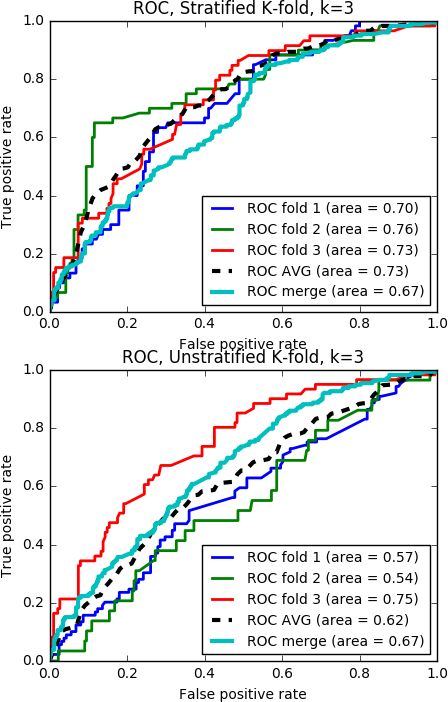
\includegraphics{./images/CV_ROC.png}
	\caption{Wykresy krzywych ROC dla klasyfikatorów ze sprawdzianu krzyżowego równomiernego i normalnego wraz z obliczoną średnią $ROC_{AVG}$ oraz $ROC_{merge}$.}
	\label{fig:cv_roc}
\end{figure}

\subsubsection{Podsumowanie}
Analizując przeprowadzone testy, najlepsze wyniki osiągnęły miary obliczone metodami opartymi na zsumowanej macierzy pomyłek oraz na łączeniu wyników testów z każdej iteracji sprawdzianu krzyżowego. Obliczone w ten sposób współczynniki miały najbardziej stabilne wyniki, najmniejszy błąd oraz wariancję. Poniżej przedstawiono tabelę (\ref{przykladoblwsp}) z obliczonymi współczynnikami na różne sposoby. Mimo równomiernego rozkładu klas, klasyfikator w części numer 2 nie rozpoznał ani jednego przykładu pozytywnego. W efekcie czułość oraz precyzja musiały zostać ustawione na 0, skutkiem czego miara G-mean oraz F1 dla tej części wynoszą 0. Pochodną tego zdarzenia jest zaniżenie wszystkich wartości średnich miar (oznaczonych w tabeli jako AVG). W dalszej części pracy, wszystkie miary w sprawdzianie krzyżowym, będą obliczane nad podstawie wspólnej macierzy pomyłek. 
\begin{table}[H]
	
	\begin{center}
		\resizebox{\textwidth}{!}{%
			\fontsize{16}{14}\selectfont
			\begin{tabular}{cccccccccccc}%
				\textbf{k-fold} & \textbf{Pos} & \textbf{Neg} & \textbf{TP} & \textbf{FP} & \textbf{FN} & \textbf{TN} & \textbf{Se} & \textbf{Sp} & \textbf{Pre} & \textbf{G-Mean} & $\mathbf{F_{1}}$\\
				\hline
				1 & 3 & 97 & 2 & 0 & 1 & 97 &  0,67 & 1,00 & 1,00 & 0,82 & 0,80\\
				2 & 3 & 97 & 0 & 0 & 3 & 97 &  0,00 & 1,00 & 0,00 & 0,00 & 0,00\\
				3 & 3 & 97 & 3 & 4 & 1 & 93 &  0,75 & 0,96 & 0,43 & 0,85 & 0,55\\

				  &   &    &   &   &   & \textbf{AVG}      & \textbf{0,47} & \textbf{0,99} & \textbf{0,48} & \textbf{0,55} & \textbf{0,45} \\
				  &   &    &   &   &   & \textbf{tp,fp,tn} & \textbf{0,50} & \textbf{0,99} & \textbf{0,56} & \textbf{0,70} & \textbf{0,53} \\
				  &   &    &   &   &   &  &  &  &  \multicolumn{3}{ c }{$\mathbf{G_{Se, Sp} =0,68}$ $\mathbf{F_{Pre, Re} =0,47}$}  \\
				

			\end{tabular}}%
			\caption{Przykład obliczonych miar dla równomiernego sprawdzianu krzyżowego. Dla k=2, gdzie nie było pozytywnie sklasyfikowanych przykładów, wartości sensitivity, precision, $F_1$ zostały ustawione na 0, aby uniknąć dzielenia przez zero. W wierszu oznaczonym jako "tp,fp,tn", wskaźniki zostały obliczone na podstawie wspólnej macierzy pomyłek.}
			\label{przykladoblwsp}
	\end{center}
\end{table}



\todo{dac odnosnik do rozdzialu}
\section{Balansowanie niezrównoważonych zbiorów ze sprawdzianem krzyżowym}
Balansowanie niezrównoważonych zbiorów danych wykonuje się w celu poprawy klasyfikacji klasy mniejszościowej. Istnieją różne techniki balansowania zbiorów(opisanych w rozdziale ), są to między innymi: usuwanie przykładów z klasy większościowej oraz dodawanie nowych obserwacji z klasy mniejszościowej. Oceniając klasyfikator z wykorzystaniem sprawdzianu krzyżowego, bilansowanie zbiorów można wykonać przed sprawdzianem krzyżowym oraz w trakcie trwania sprawdzianu, każdorazowo po stworzeniu zbioru uczącego. W przypadku generowania nowych obserwacji (oversampling), metoda pierwsza może prowadzić do nadmiernego dopasowania. Sprawdzian krzyżowy k-krotny, dzieli główny zbiór danych na $k$ części i buduje klasyfikator w oparciu $k-1$ części. Następnie testuje go w oparciu o część numer $k$. Może wystąpić sytuacja, że ocena klasyfikatora będzie odbywała się w oparciu o sztuczne przykłady, które były wygenerowane na podstawie danych tworzących zbiór uczący. Takie zdarzenie wypacza cel wykonywania sprawdzianu krzyżowego, który polega na wykonywaniu uczenia i testowania na różnych danych. Wykonanie bilansowania przed sprawdzianem krzyżowym może prowadzić do nadmiernego dopasowania klasyfikatora oraz do zawyżenia oceny. 
\begin{figure}[H]
	\centering
	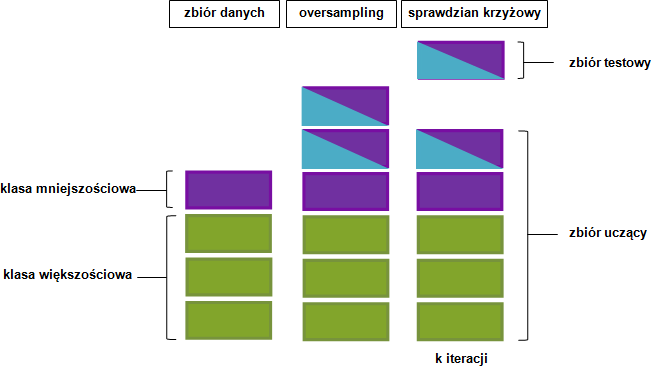
\includegraphics[width=\textwidth]{./images/oversampling.png}
	\caption{Przykład sprawdzianu krzyżowego z wykonanym oversamplingiem przed sprawdzianem. Sztucznie wygenerowane dane (niebiesko-fioletowy prostokąt) zostały użyte jako zbiór testowy.}
	\label{fig:oversampling_wrong}
\end{figure}
Celem testu było sprawdzenie, z wykorzystaniem, której metody można otrzymać bardziej wiarygodne wyniki. Aby sprawdzić obie metody, każdy początkowy zbiór danych został podzielony na zbiór testowy (zawierający 80\% wszystkich przykładów) oraz na zbiór walidacyjny (20\%). Wykonano zbilansowany podział danych, tj. każdy zbiór zawierał proporcjonalnie takie same ilości obu klas. Zbiór walidacyjny został wydzielony w celu poddania dodatkowej ocenie każdego $k$ klasyfikatora. Mając dodatkowy zbiór walidacyjny, który jest nieznany zbudowanemu modelowi, można sprawdzić w jakim stopniu poprawnie generalizuje dane uczące oraz porównać otrzymane wyniki z wynikami sprawdzianu krzyżowego. Dla pierwszego sposobu, w kolejnym etapie, wygenerowano nowe sztuczne próbki klasy mniejszościowej z wykorzystaniem metody oversampling SMOTE, a następnie poddano ocenie klasyfikator z wykorzystaniem sprawdzianu krzyżowego oraz dodatkowego zbioru walidacyjnego w każdej iteracji. Natomiast w drugim sposobie, dodatkowe sztuczne próbki generowane były dopiero w momencie utworzenia $k$ zbioru uczącego. Dodatkowa walidacja odbywała się tak samo jak w pierwszym sposobie. Badanie wykonano na prawdziwych danych (opisanych w tej pracy), z wykorzystaniem klasyfikatorów: drzewo decyzyjne, kNN, naiwny klasyfikator Bayesa oraz SVM. Przedstawiony niżej test znajduje się w pliku $cross\_val\_oversampling.py$. Ze względu na dużą objętość wyników, w pracy przedstawiono tylko dane dla drzewa decyzyjnego. \par
Analizując otrzymane wyniki (tabela \ref{CVoversampling1} i \ref{CVoversampling2}) zauważono bardzo dobre wyniki klasyfikatora dla danych poddanych oversamplingowi przed sprawdzianem krzyżowym. Niestety, badając klasyfikator nieznanym dla niego zbiorem walidacyjnym otrzymane rezultaty były zdecydowanie gorsze. Porównując otrzymane wyniki ze sprawdzianu krzyżowego oraz z nieznanego klasyfikatorowi zbioru walidacyjnyjego, spostrzeżono znaczne zawyżanie wyników (dla miary G-mean, wyniki jest średnio wyższy o 0.20 oraz tak samo w stosunku do miary G-mean z metody drugiej). Świadczy to o nadmiernym dopasowaniu klasyfikatora do danych i o zawyżaniu wyników jakości klasyfikacji przez tą metodę. W drugiej metodzie, wyniki pomiarów pomiędzy sprawdzianem krzyżowym oraz zbiorem walidacyjnym nie różnią się tak bardzo. Dla miary G-mean w większości baz, otrzymany wyniki z sprawdzianu krzyżowego jest nieznacznie niższy od wyniku z zbioru walidacyjnego. \par
Wnioskiem wynikającym z powyższego badania jest konieczność stosowania oversamplingu danych w trakcie sprawdzianu krzyżowego, tak aby zbiór testowy nie zawierał sztucznie wygenerowanych próbek. Ocena klasyfikacji tą metodą, daje najbardziej wiarygodne wyniki.
\begin{table}[H]
	\begin{center}
		\resizebox{\textwidth}{!}{%
			\begin{tabular}{|c|c|c|c|c|c|c|c|c|c|}%
				\hline%
				&\multicolumn{4}{|c|}{Decision Tree}&\multicolumn{4}{|c|}{Decision Tree TEST}&\\%
				\cline{2%
					-%
					10}%
				& Sp & F1 & G & AUC & Sp &F1 & $G_t$&AUC& $G - G_t$\\%
				\hline%
				abalone0\_4&0.99&0.99&0.99&0.99&0.79&0.58&0.88&0.88&0.11\\%
				abalone041629&0.92&0.91&0.9&0.9&0.5&0.34&0.66&0.69&0.24\\%
				abalone16\_29&0.93&0.92&0.92&0.92&0.51&0.34&0.68&0.71&0.24\\%
				balance\_scale&0.92&0.9&0.9&0.9&0.04&0.04&0.19&0.47&0.71\\%
				breast\_cancer&0.74&0.74&0.74&0.75&0.47&0.45&0.59&0.61&0.15\\%
				bupa&0.69&0.66&0.65&0.65&0.57&0.55&0.6&0.6&0.05\\%
				car&1.0&1.0&1.0&1.0&0.9&0.95&0.95&0.95&0.05\\%
				cmc&0.8&0.81&0.81&0.81&0.39&0.37&0.55&0.6&0.26\\%
				ecoli&0.93&0.93&0.92&0.93&0.81&0.62&0.86&0.86&0.06\\%
				german&0.74&0.75&0.75&0.75&0.44&0.44&0.58&0.59&0.17\\%
				glass&0.96&0.93&0.93&0.93&0.56&0.5&0.73&0.75&0.2\\%
				haberman&0.72&0.73&0.74&0.74&0.35&0.35&0.52&0.56&0.22\\%
				heart\_cleveland&0.88&0.87&0.86&0.86&0.24&0.29&0.47&0.59&0.39\\%
				hepatitis&0.92&0.86&0.84&0.85&0.39&0.33&0.54&0.57&0.3\\%
				horse\_colic&0.84&0.82&0.82&0.82&0.65&0.66&0.73&0.73&0.09\\%
				ionosphere&0.88&0.88&0.88&0.88&0.87&0.81&0.86&0.86&0.02\\%
				new\_thyroid&0.96&0.96&0.96&0.96&1.0&0.95&0.99&0.99&{-}0.03\\%
				postoperative&0.68&0.7&0.71&0.71&0.33&0.34&0.51&0.56&0.2\\%
				seeds&0.97&0.96&0.96&0.96&0.62&0.7&0.76&0.77&0.2\\%
				solar\_flare&0.96&0.96&0.96&0.97&0.13&0.19&0.36&0.63&0.6\\%
				transfusion&0.76&0.75&0.75&0.77&0.4&0.35&0.54&0.58&0.21\\%
				vehicle&0.89&0.92&0.92&0.92&0.72&0.76&0.83&0.83&0.09\\%
				vertebal&0.89&0.86&0.85&0.85&0.73&0.66&0.75&0.75&0.1\\%
				yeastME1&0.99&0.99&0.99&0.99&0.72&0.68&0.84&0.85&0.15\\%
				yeastME2&0.98&0.96&0.96&0.96&0.69&0.42&0.81&0.82&0.15\\%
				yeastME3&0.96&0.96&0.96&0.96&0.66&0.65&0.79&0.81&0.17\\%
				\hline%
			\end{tabular}}%
			\caption{Wyniki sprawdzianu krzyżowego (metoda pierwsza) drzewa decyzyjnego z oversampling SMOTE. Dane w kolumnach "Decision Tree TEST" to wyniki otrzymane na podstawie zbioru walidacyjnego. Ostatnia kolumna zawiera różnicę  miar G ze sprawdzianu krzyżowego i zbioru walidacyjnego $G-G_T$ (im bliżej zera tym lepiej).}
			\label{CVoversampling1}
		\end{center}
\end{table}


\begin{table}[H]
	\begin{center}
		\resizebox{\textwidth}{!}{%
		\begin{tabular}{|c|c|c|c|c|c|c|c|c|c|}%
			\hline%
			&\multicolumn{4}{|c|}{Decision Tree}&\multicolumn{4}{|c|}{Decision Tree TEST}&\\%
			\cline{2%
				-%
				10}%
				& Sp & F1 & G & AUC & Sp &F1 & $G_t$&AUC& $G - G_t$\\%
			\hline%
			abalone0\_4&0.68&0.54&0.82&0.83&0.77&0.58&0.87&0.88&{-}0.05\\%
			abalone041629&0.42&0.31&0.61&0.65&0.45&0.32&0.63&0.67&{-}0.02\\%
			abalone16\_29&0.39&0.27&0.59&0.64&0.52&0.34&0.68&0.71&{-}0.09\\%
			balance\_scale&0.03&0.02&0.15&0.47&0.04&0.03&0.19&0.46&{-}0.04\\%
			breast\_cancer&0.41&0.4&0.55&0.57&0.41&0.4&0.55&0.57&0.0\\%
			bupa&0.54&0.54&0.6&0.6&0.55&0.56&0.62&0.62&{-}0.02\\%
			car&0.98&0.98&0.99&0.99&0.91&0.95&0.95&0.95&0.04\\%
			cmc&0.38&0.36&0.55&0.59&0.39&0.37&0.56&0.61&{-}0.01\\%
			ecoli&0.54&0.53&0.71&0.74&0.62&0.58&0.76&0.78&{-}0.05\\%
			german&0.55&0.54&0.66&0.67&0.5&0.49&0.62&0.63&0.04\\%
			glass&0.14&0.16&0.37&0.54&0.56&0.56&0.73&0.76&{-}0.36\\%
			haberman&0.49&0.42&0.58&0.59&0.4&0.36&0.53&0.55&0.05\\%
			heart\_cleveland&0.43&0.35&0.61&0.65&0.24&0.29&0.48&0.59&0.13\\%
			hepatitis&0.5&0.52&0.67&0.69&0.72&0.58&0.77&0.77&{-}0.1\\%
			horse\_colic&0.78&0.77&0.82&0.82&0.65&0.66&0.73&0.73&0.09\\%
			ionosphere&0.82&0.81&0.85&0.85&0.85&0.81&0.85&0.85&0.0\\%
			new\_thyroid&0.88&0.86&0.92&0.92&0.94&0.87&0.95&0.95&{-}0.03\\%
			postoperative&0.32&0.27&0.44&0.48&0.33&0.3&0.47&0.48&{-}0.03\\%
			seeds&0.95&0.91&0.94&0.94&0.62&0.68&0.75&0.76&0.19\\%
			solar\_flare&0.21&0.2&0.45&0.62&0.13&0.18&0.36&0.63&0.09\\%
			transfusion&0.36&0.34&0.52&0.58&0.39&0.35&0.54&0.57&{-}0.02\\%
			vehicle&0.82&0.82&0.88&0.88&0.76&0.79&0.85&0.85&0.03\\%
			vertebal&0.66&0.68&0.75&0.76&0.63&0.63&0.72&0.73&0.03\\%
			yeastME1&0.63&0.59&0.79&0.81&0.72&0.69&0.84&0.86&{-}0.05\\%
			yeastME2&0.29&0.2&0.53&0.62&0.41&0.3&0.63&0.68&{-}0.1\\%
			yeastME3&0.81&0.77&0.88&0.89&0.68&0.68&0.81&0.82&0.07\\%
			\hline%
		\end{tabular}}%
			\caption{Wyniki sprawdzianu krzyżowego (metoda druga) drzewa decyzyjnego z oversampling SMOTE. Dane w kolumnach "Decision Tree TEST" to wyniki otrzymane na podstawie zbioru walidacyjnego. Ostatnia kolumna zawiera różnicę  miar G ze sprawdzianu krzyżowego i zbioru walidacyjnego $G-G_T$ (im bliżej zera tym lepiej).}
			\label{CVoversampling2}
	\end{center}
\end{table}
\chapter{Meta-metody}
\section{Bagging}
Klasyfikator bagging to meta-klasyfikator, który trenuje $n$ klasyfikatorów bazowych na losowych podzbiorach oryginalnego zbioru danych, a~następnie poprzez głosowanie lub uśrednianie indywidualnych prognoz nadaje ostateczną klasę. W procesie tworzenia klasyfikatora bagging, należy wybrać klasyfikator bazowy oraz określić liczbę $n$ tworzonych instancji tego klasyfikatora. Można także zdefiniować, czy losowe podzbiory mają być tworzone próbą boostrap, maksymalną liczebność podzbiorów oraz liczebność atrybutów. Zmieniając liczbę estymatorów, liczebność podzbiorów oraz atrybutów wpływa się na jakość klasyfikacji. Badania przeprowadzono z~wykorzystaniem trzech różnych klasyfikatorów bazowych tj. z~drzewem decyzyjnym, naiwnym klasyfikatorem bayesowskim, klasyfikatorem k najbliższych sąsiadów oraz dla różnych wartości przykładów oraz atrybutów. Każdy test został przeprowadzony z~wykorzystaniem 5, 10, 15, 30, 50, 100 i~200 estymatorów. Wszystkie podzbiory zostały utworzone z~wykorzystaniem próby boostrap, zatem podzbiory z~taką samą liczebnością jak zbiór główny, będą różniły się od siebie próbkami.
  
\subsection{Bagging z~naiwnym klasyfikatorem bayesowskim}
Zbudowano klasyfikator bagging z~naiwnym klasyfikatorem Bayesa (NKB). Test ten znajduje się w~pliku \textit{bagging\_NB.py}. W pierwszym etapie badań wybrano standardowe ustawienia, czyli liczebność podzbiorów (\textit{max\_samples}) oraz atrybutów (\textit{max\_features}) była taka sama jak w~zbiorze oryginalnym.
W tabelach poniżej przedstawiono dokładność klasyfikacji (tabela \ref{bagging_11}) oraz specyficzność klasy mniejszościowej (tabela \ref{bagging-specyficznosc11}). W kolumnie drugiej znajdują się wyniki dla samego naiwnego klasyfikatora Bayesa, natomiast w~kolejnych kolumnach znajdują się wyniki meta-klasyfikatora bagging z~różną liczbą modeli bazowych (dla 5, 10, 15, 30, 50, 100, 200 klasyfikatorów). Analizując otrzymane wyniki, zauważono tylko minimalny wzrost (około 1\%) poprawy klasyfikacji obu klas dla połowy zbiorów danych. Dla prawie wszystkich zbiorów danych wartość miary G-mean zmieniła się minimalnie, poniżej błędu. Test został wykonany wielokrotnie, a~otrzymywane wyniki różniły się w~bardzo niewielkim stopniu. 
\begin{table}[H]
	\tiny
	\begin{center}
		\resizebox{0.90\textwidth}{!}{%
			\begin{tabular}{c|cccccccc}%
				Zbiór danych&NKB&5&10&15&30&50&100&200\\%
				\hline%
				seeds&\textbf{0.9}&\textbf{0.9}&\textbf{0.9}&\textbf{0.9}&\textbf{0.9}&\textbf{0.9}&\textbf{0.9}&\textbf{0.9}\\%
				
				new\_thyroid&0.96&0.96&\textbf{0.97}&\textbf{0.97}&\textbf{0.97}&0.96&0.96&0.96\\%
				
				vehicle&0.66&\textbf{0.67}&\textbf{0.67}&\textbf{0.67}&\textbf{0.67}&0.66&0.66&0.66\\%
				
				ionosphere&\textbf{0.87}&0.85&0.85&0.85&0.86&0.86&\textbf{0.87}&\textbf{0.87}\\%
				
				vertebal&\textbf{0.78}&0.77&0.77&0.77&0.77&0.77&\textbf{0.78}&0.77\\%
				
				yeastME3&\textbf{0.27}&0.17&0.21&0.23&0.25&0.25&0.25&0.25\\%
				
				ecoli&0.78&0.77&0.79&\textbf{0.8}&0.79&0.79&0.78&0.79\\%
				
				bupa&0.54&0.53&\textbf{0.55}&0.54&\textbf{0.55}&\textbf{0.55}&0.54&0.54\\%
				
				horse\_colic&\textbf{0.78}&0.76&0.77&0.77&0.77&0.77&\textbf{0.78}&0.77\\%
				
				german&\textbf{0.73}&\textbf{0.73}&\textbf{0.73}&\textbf{0.73}&0.72&0.72&0.72&0.72\\%
				
				breast\_cancer&\textbf{0.72}&\textbf{0.72}&0.71&0.71&\textbf{0.72}&\textbf{0.72}&\textbf{0.72}&\textbf{0.72}\\%
				
				cmc&\textbf{0.68}&\textbf{0.68}&\textbf{0.68}&\textbf{0.68}&\textbf{0.68}&\textbf{0.68}&\textbf{0.68}&\textbf{0.68}\\%
				
				hepatitis&0.66&0.65&0.65&0.66&\textbf{0.68}&\textbf{0.68}&\textbf{0.68}&\textbf{0.68}\\%
				
				haberman&0.73&\textbf{0.74}&\textbf{0.74}&\textbf{0.74}&\textbf{0.74}&\textbf{0.74}&\textbf{0.74}&\textbf{0.74}\\%
				
				transfusion&\textbf{0.74}&\textbf{0.74}&\textbf{0.74}&\textbf{0.74}&\textbf{0.74}&\textbf{0.74}&\textbf{0.74}&\textbf{0.74}\\%
				
				car&0.89&\textbf{0.91}&0.9&0.9&0.9&0.9&0.9&0.9\\%
				
				glass&0.48&0.48&0.49&\textbf{0.53}&0.48&0.49&0.49&0.5\\%
				
				abalone16\_29&0.68&0.68&0.68&\textbf{0.69}&0.68&0.68&0.68&0.68\\%
				
				solar\_flare&\textbf{0.65}&0.62&0.61&0.63&0.62&0.62&0.62&0.63\\%
				
				heart\_cleveland&\textbf{0.81}&0.8&\textbf{0.81}&0.8&\textbf{0.81}&\textbf{0.81}&0.8&0.8\\%
				
				balance\_scale&\textbf{0.92}&\textbf{0.92}&\textbf{0.92}&\textbf{0.92}&\textbf{0.92}&\textbf{0.92}&\textbf{0.92}&\textbf{0.92}\\%
				
				postoperative&\textbf{0.67}&0.62&0.64&0.62&0.6&0.61&0.62&0.63\\%
				
			\end{tabular}}
			\caption{Dokładność klasyfikatora bagging NKB, dla \textit{max\_features = 1.0} oraz \textit{max\_samples = 1.0}.}
			\label{bagging_11}
		\end{center}
	\end{table}
	\begin{table}[H]
		\tiny
		\begin{center}
			\resizebox{0.90\textwidth}{!}{%
				\begin{tabular}{c|cccccccc}%
					Zbiór danych&NKB&5&10&15&30&50&100&200\\%
					\hline%
					seeds&\textbf{0.91}&\textbf{0.91}&\textbf{0.91}&\textbf{0.91}&\textbf{0.91}&\textbf{0.91}&\textbf{0.91}&\textbf{0.91}\\%
					
					new\_thyroid&\textbf{0.87}&\textbf{0.87}&\textbf{0.87}&\textbf{0.87}&\textbf{0.87}&\textbf{0.87}&\textbf{0.87}&\textbf{0.87}\\%
					
					vehicle&0.84&0.83&0.84&0.84&\textbf{0.85}&0.84&0.84&0.84\\%
					
					ionosphere&0.76&0.76&\textbf{0.77}&\textbf{0.77}&\textbf{0.77}&0.76&0.76&0.76\\%
					
					vertebal&\textbf{0.87}&0.86&0.86&0.86&0.86&0.86&\textbf{0.87}&0.86\\%
					
					yeastME3&\textbf{0.99}&\textbf{0.99}&\textbf{0.99}&\textbf{0.99}&\textbf{0.99}&\textbf{0.99}&\textbf{0.99}&\textbf{0.99}\\%
					
					ecoli&\textbf{0.94}&\textbf{0.94}&\textbf{0.94}&\textbf{0.94}&\textbf{0.94}&\textbf{0.94}&\textbf{0.94}&\textbf{0.94}\\%
					
					bupa&0.74&0.75&\textbf{0.77}&\textbf{0.77}&0.74&0.75&0.75&0.74\\%
					
					horse\_colic&\textbf{0.75}&\textbf{0.75}&0.74&\textbf{0.75}&\textbf{0.75}&0.74&0.74&0.73\\%
					
					german&0.62&0.6&0.6&0.6&0.63&0.63&\textbf{0.65}&\textbf{0.65}\\%
					
					breast\_cancer&0.44&0.45&0.44&0.44&\textbf{0.46}&\textbf{0.46}&\textbf{0.46}&\textbf{0.46}\\%
					
					cmc&0.61&0.61&0.61&0.61&\textbf{0.62}&\textbf{0.62}&\textbf{0.62}&0.61\\%
					
					hepatitis&\textbf{0.78}&0.72&0.72&0.75&0.75&0.75&0.75&0.75\\%
					
					haberman&0.17&\textbf{0.2}&0.19&0.19&\textbf{0.2}&\textbf{0.2}&\textbf{0.2}&\textbf{0.2}\\%
					
					transfusion&0.2&\textbf{0.21}&\textbf{0.21}&\textbf{0.21}&\textbf{0.21}&\textbf{0.21}&\textbf{0.21}&\textbf{0.21}\\%
					
					car&\textbf{1.0}&\textbf{1.0}&\textbf{1.0}&\textbf{1.0}&\textbf{1.0}&\textbf{1.0}&\textbf{1.0}&\textbf{1.0}\\%
					
					glass&0.82&0.82&0.82&0.82&\textbf{0.88}&\textbf{0.88}&\textbf{0.88}&0.82\\%
					
					abalone16\_29&0.58&\textbf{0.59}&0.58&0.58&0.58&0.58&0.58&0.58\\%
					
					solar\_flare&\textbf{0.93}&\textbf{0.93}&\textbf{0.93}&\textbf{0.93}&\textbf{0.93}&\textbf{0.93}&\textbf{0.93}&\textbf{0.93}\\%
					
					heart\_cleveland&\textbf{0.63}&0.57&0.6&0.57&0.6&0.57&0.57&0.57\\%
					
					balance\_scale&\textbf{0.0}&\textbf{0.0}&\textbf{0.0}&\textbf{0.0}&\textbf{0.0}&\textbf{0.0}&\textbf{0.0}&\textbf{0.0}\\%
					
					postoperative&0.17&\textbf{0.21}&\textbf{0.21}&\textbf{0.21}&0.12&0.12&0.12&0.12\\%
					
				\end{tabular}}
				\caption{Specyficzność klasy mniejszościowej, dla klasyfikatora bagging NKB i~parametrów: \textit{max\_features = 1.0} oraz \textit{max\_samples = 1.0}.}
				\label{bagging-specyficznosc11}
			\end{center}
		\end{table}
\par
W kolejnym teście znajdującym się w~pliku \textit{gridsearch/bagging\_NB.py}, wykonano zachłanne obliczenia polegające na wyłonieniu najlepszych ustawień klasyfikatora maksymalizującego miarę $F_1$ klasy mniejszościowej. W tym celu wykonano wyszukiwanie zachłanne najlepszych parametrów (liczby atrybutów oraz liczebności zbiorów) spośród \textit{max\_features=[0.4, 0.6, 0.7, 0.8, 0.9, 1.0]} oraz \textit{max\_samples=[0.4, 0.6, 0.7, 0.8, 0.9, 1.0]}. Wyszukanie wykonano dla n-klasyfikatorów ze zbioru \textit{[5, 10, 15, 30, 50, 100, 200]} oraz dla każdego zbioru danych. Obliczona średnia wartość parametru \textit{max\_features} wyniosła 0.72, a~\textit{max\_samples} 0.68, zaś mediana dla obu wartości to 0.7. \par
Zbudowany meta-klasyfikator bagging z~parametrami \textit{max\_features=0.72} i~\textit{max\_samples=0.68} poradził sobie lepiej z~klasyfikacją niż klasyfikator bagging z~domyślnymi parametrami oraz zwykły klasyfikator. W przypadku 17 zbiorów danych osiągnął lepszą dokładność (tabela \ref{bagging_acc2}). Dokładność klasyfikacji wzrosła średnio o~2-3\%, a~w 3 zbiorach wzrost był zdecydowanie większy. Natomiast w~5 zbiorach danych, klasyfikator bagging uzyskał taką samą lub minimalne gorszą dokładność. W zespołach liczących powyżej 10 klasyfikatorów wystąpił minimalny przyrost dokładności poniżej 1\%. Prawie dla wszystkich danych, zwiększyła się czułość klasy większościowej, kosztem specyficzności (tabela \ref{baggin_spec2}) klasy mniejszościowej. Podobnie jak dla poprzedniego klasyfikatora, miara G-mean minimalnie spadła lub wzrosła w~stosunku do NKB.
\begin{table}[H]
	\tiny
	\begin{center}
		\resizebox{\textwidth}{!}{%
			\begin{tabular}{c|cccccccc}%

				Zbiór danych&NKB&5&10&15&30&50&100&200\\%
				\hline%
				seeds&0.9&0.89&0.9&\textbf{0.91}&\textbf{0.91}&\textbf{0.91}&0.9&0.9\\%
				new\_thyroid&0.96&\textbf{0.97}&\textbf{0.97}&\textbf{0.97}&\textbf{0.97}&\textbf{0.97}&\textbf{0.97}&\textbf{0.97}\\%
				vehicle&0.66&0.68&0.68&0.67&\textbf{0.69}&0.67&0.67&0.68\\%
				ionosphere&\textbf{0.87}&0.83&0.86&0.83&\textbf{0.87}&\textbf{0.87}&0.86&0.86\\%
				vertebal&\textbf{0.78}&0.75&0.76&0.77&0.77&0.77&0.77&\textbf{0.78}\\%
				yeastME3&0.27&\textbf{0.34}&0.25&0.17&0.21&0.23&0.23&0.22\\%
				ecoli&0.78&0.83&0.8&0.8&0.81&0.83&\textbf{0.84}&0.83\\%
				bupa&0.54&0.57&0.57&\textbf{0.6}&\textbf{0.6}&0.59&0.59&\textbf{0.6}\\%
				horse\_colic&0.78&0.73&0.76&0.73&0.76&0.77&0.78&\textbf{0.79}\\%
				german&\textbf{0.73}&0.66&0.66&0.68&0.7&0.72&0.72&\textbf{0.73}\\%
				breast\_cancer&0.72&\textbf{0.73}&\textbf{0.73}&\textbf{0.73}&\textbf{0.73}&\textbf{0.73}&\textbf{0.73}&\textbf{0.73}\\%
				cmc&0.68&\textbf{0.72}&0.71&0.71&0.71&0.71&\textbf{0.72}&\textbf{0.72}\\%
				hepatitis&0.66&0.63&0.67&\textbf{0.68}&0.66&0.66&\textbf{0.68}&0.67\\%
				haberman&0.73&0.74&\textbf{0.75}&\textbf{0.75}&0.74&0.74&0.74&0.74\\%
				transfusion&0.74&0.76&0.75&0.75&0.75&\textbf{0.77}&\textbf{0.77}&\textbf{0.77}\\%
				car&0.89&\textbf{0.92}&0.9&0.9&0.9&0.9&0.9&0.9\\%
				glass&0.48&\textbf{0.76}&0.59&0.61&0.59&0.6&0.6&0.59\\%
				abalone16\_29&0.68&0.8&\textbf{0.81}&0.8&0.79&0.79&0.79&0.79\\%
				solar\_flare&\textbf{0.65}&0.6&0.53&0.52&0.64&0.58&0.53&0.58\\%
				heart\_cleveland&0.81&0.78&0.8&0.81&0.82&0.82&\textbf{0.83}&0.82\\%
				balance\_scale&\textbf{0.92}&\textbf{0.92}&\textbf{0.92}&\textbf{0.92}&\textbf{0.92}&\textbf{0.92}&\textbf{0.92}&\textbf{0.92}\\%
				postoperative&0.67&\textbf{0.69}&0.63&0.62&0.64&0.62&0.63&0.64\\%
				\end{tabular}}
			\caption{Dokładność klasyfikatora bagging NKB, dla \textit{max\_features = 0.72} oraz \textit{max\_samples = 0.68}.}
			\label{bagging_acc2}
		\end{center}
	\end{table}
\begin{table}[H]
		\tiny
	\begin{center}
		\resizebox{\textwidth}{!}{%
			\begin{tabular}{c|cccccccc}%

				Zbiór danych&NKB&5&10&15&30&50&100&200\\%
				\hline%
				seeds&\textbf{0.91}&0.89&\textbf{0.91}&\textbf{0.91}&\textbf{0.91}&\textbf{0.91}&\textbf{0.91}&\textbf{0.91}\\%
				new\_thyroid&\textbf{0.87}&0.8&\textbf{0.87}&\textbf{0.87}&\textbf{0.87}&\textbf{0.87}&\textbf{0.87}&\textbf{0.87}\\%
				vehicle&0.84&\textbf{0.85}&0.82&0.83&0.82&0.82&0.82&0.83\\%
				ionosphere&0.76&\textbf{0.83}&0.75&0.79&0.75&0.73&0.72&0.74\\%
				vertebal&\textbf{0.87}&0.81&0.83&0.86&0.86&0.86&0.84&0.86\\%
				yeastME3&\textbf{0.99}&\textbf{0.99}&\textbf{0.99}&\textbf{0.99}&\textbf{0.99}&\textbf{0.99}&\textbf{0.99}&\textbf{0.99}\\%
				ecoli&\textbf{0.94}&0.83&0.86&0.8&0.91&0.91&0.91&0.91\\%
				bupa&\textbf{0.74}&0.5&0.63&0.62&0.64&0.7&0.67&0.67\\%
				horse\_colic&0.75&0.72&0.74&0.75&0.75&0.75&\textbf{0.76}&\textbf{0.76}\\%
				german&0.62&\textbf{0.73}&0.71&0.69&0.69&0.64&0.63&0.64\\%
				breast\_cancer&\textbf{0.44}&0.39&\textbf{0.44}&\textbf{0.44}&\textbf{0.44}&\textbf{0.44}&0.42&0.42\\%
				cmc&\textbf{0.61}&0.51&0.53&0.5&0.52&0.5&0.48&0.5\\%
				hepatitis&0.78&\textbf{0.84}&0.75&0.75&0.72&0.72&0.75&0.75\\%
				haberman&0.17&0.1&\textbf{0.19}&0.16&0.17&0.16&0.14&0.14\\%
				transfusion&\textbf{0.2}&0.15&0.16&0.17&0.15&0.16&0.16&0.16\\%
				car&\textbf{1.0}&0.45&\textbf{1.0}&\textbf{1.0}&\textbf{1.0}&\textbf{1.0}&\textbf{1.0}&\textbf{1.0}\\%
				glass&\textbf{0.82}&0.59&0.76&0.71&0.71&0.71&0.76&0.76\\%
				abalone16\_29&\textbf{0.58}&0.28&0.4&0.42&0.43&0.43&0.44&0.43\\%
				solar\_flare&\textbf{0.93}&0.81&\textbf{0.93}&\textbf{0.93}&\textbf{0.93}&\textbf{0.93}&\textbf{0.93}&\textbf{0.93}\\%
				heart\_cleveland&\textbf{0.63}&0.57&0.54&0.49&0.46&0.46&0.51&0.46\\%
				balance\_scale&\textbf{0.0}&\textbf{0.0}&\textbf{0.0}&\textbf{0.0}&\textbf{0.0}&\textbf{0.0}&\textbf{0.0}&\textbf{0.0}\\%
				postoperative&\textbf{0.17}&\textbf{0.17}&0.12&0.12&\textbf{0.17}&0.12&0.08&0.12\\%
			\end{tabular}}
			\caption{Specyficzność klasy mniejszościowej, dla klasyfikatora bagging NKB i~parametrów: \textit{max\_features = 0.72} oraz \textit{max\_samples = 0.68}.}
			\label{baggin_spec2}
		\end{center}
	\end{table}
\subsection{Bagging drzewa decyzyjne}
Do kolejnych testów z~meta-klasyfikatorem bagging wybrano drzewo decyzyjne. Budując klasyfikator drzewa decyzyjnego można zdefiniować maksymalną głębokość drzewa. Również meta-klasyfikator bagging można zbudować z~drzew o~różnej maksymalnej głębokości. Do testów wybrano drzewo bez ograniczenia głębokości oraz drzewa z~ograniczeniami do maksymalnie 3, 5, 7, 10, 15 i~20 poziomu. Meta-klasyfikator był budowany z~5, 10, 20 lub 50 klasyfikatorów. Dla porównania, w~wynikach zamieszczono pojedyncze drzewo decyzyjne o~różnej głębokości. Przeprowadzony test znajduje się w~pliku \textit{bagging\_tree.py}. Ze względu na dużą objętość tabel pominięto wyniki niektórych zbiorów danych. Dla bazy \textit{seeds} i~\textit{new\_thyroid}, dokładność klasyfikacji i~wykrywalność klas pozostała na takim samym poziomie niezależnie od głębokości drzewa i~liczby klasyfikatorów. Natomiast w~przypadku baz \textit{vehicle}, \textit{ionosphere}, \textit{vertebal}, \textit{yeastME3}, \textit{solar\_flare} klasyfikator bagging zwiększył dokładność klasyfikacji średnio o~2-3\%, czułość pozostała na niezmienionym poziomie, wzrosła natomiast specyficzność klasy mniejszościowej o~2-3\% oraz miara G-mean. Należy zaznaczyć, że dokładność oraz pozostałe współczynniki rosły wraz ze zwiększeniem liczebności klasyfikatorów. Powyżej 50 klasyfikatorów przyrost był minimalny. Dokładność klasyfikatora baggging dla pozostałych baz została przedstawiona w~tabeli \ref{baggingdrzewoacc}. W tabelach \ref{baggingdrzewoacc} i~\ref{baggingdrzewospec} w~kolumnach znajdują się klasyfikatory z~różną maksymalną głębokością drzewa, a~znak '-' oznacza drzewo bez ograniczenia. 
\begin{table}[H]
	\tiny
	\begin{center}
		\resizebox{\textwidth}{!}{%
			\begin{tabular}{c|c|ccccccc}%
				\hline%
				Zbiór danych&Liczba est.&{-}&3&5&7&10&15&20\\%
				\hline%
				\multirow{5}{*}{breast\_cancer}&{-}&0.63&\textbf{0.73}&0.72&0.67&0.66&0.63&0.63\\%
				\cline{2%
					-%
					9}%
				&5&0.68&\textbf{0.7}&\textbf{0.7}&0.67&0.67&0.68&0.68\\%
				\cline{2%
					-%
					9}%
				&10&\textbf{0.71}&\textbf{0.71}&0.7&0.67&\textbf{0.71}&\textbf{0.71}&\textbf{0.71}\\%
				\cline{2%
					-%
					9}%
				&20&0.71&0.71&0.72&0.71&\textbf{0.74}&0.71&0.71\\%
				\cline{2%
					-%
					9}%
				&50&0.7&\textbf{0.72}&\textbf{0.72}&0.7&0.71&0.71&0.7\\%
				\hline%
				\multirow{5}{*}{cmc}&{-}&0.68&\textbf{0.78}&0.76&0.71&0.72&0.68&0.68\\%
				\cline{2%
					-%
					9}%
				&5&0.71&\textbf{0.78}&0.77&0.76&0.73&0.71&0.71\\%
				\cline{2%
					-%
					9}%
				&10&0.73&\textbf{0.77}&\textbf{0.77}&0.76&0.74&0.73&0.73\\%
				\cline{2%
					-%
					9}%
				&20&0.74&\textbf{0.78}&0.77&0.77&0.75&0.74&0.74\\%
				\cline{2%
					-%
					9}%
				&50&0.75&\textbf{0.78}&0.77&0.77&0.76&0.74&0.75\\%
				\hline%
				\multirow{5}{*}{hepatitis}&{-}&0.66&0.66&\textbf{0.68}&0.66&0.66&0.66&0.66\\%
				\cline{2%
					-%
					9}%
				&5&0.68&\textbf{0.7}&0.68&0.68&0.68&0.68&0.68\\%
				\cline{2%
					-%
					9}%
				&10&0.75&0.75&\textbf{0.77}&0.75&0.75&0.75&0.75\\%
				\cline{2%
					-%
					9}%
				&20&\textbf{0.72}&0.7&\textbf{0.72}&\textbf{0.72}&\textbf{0.72}&\textbf{0.72}&\textbf{0.72}\\%
				\cline{2%
					-%
					9}%
				&50&\textbf{0.7}&0.69&\textbf{0.7}&\textbf{0.7}&\textbf{0.7}&\textbf{0.7}&\textbf{0.7}\\%
				\hline%
				\multirow{5}{*}{haberman}&{-}&0.66&\textbf{0.75}&\textbf{0.75}&0.73&0.63&0.66&0.66\\%
				\cline{2%
					-%
					9}%
				&5&0.66&\textbf{0.74}&0.73&0.69&0.67&0.66&0.66\\%
				\cline{2%
					-%
					9}%
				&10&0.66&0.72&\textbf{0.74}&0.72&0.65&0.66&0.66\\%
				\cline{2%
					-%
					9}%
				&20&0.66&0.73&\textbf{0.74}&0.68&0.67&0.66&0.66\\%
				\cline{2%
					-%
					9}%
				&50&0.68&\textbf{0.74}&0.73&0.71&0.69&0.68&0.68\\%
				\hline%
				\multirow{5}{*}{glass}&{-}&0.7&\textbf{0.82}&0.75&0.69&0.7&0.7&0.7\\%
				\cline{2%
					-%
					9}%
				&5&0.73&\textbf{0.86}&0.78&0.73&0.73&0.73&0.73\\%
				\cline{2%
					-%
					9}%
				&10&0.84&\textbf{0.86}&0.83&0.84&0.84&0.84&0.84\\%
				\cline{2%
					-%
					9}%
				&20&0.86&\textbf{0.89}&0.87&0.86&0.86&0.86&0.86\\%
				\cline{2%
					-%
					9}%
				&50&0.86&\textbf{0.88}&0.87&0.86&0.86&0.86&0.86\\%
				\hline%
				\multirow{5}{*}{abalone16\_29}&{-}&0.91&\textbf{0.94}&0.93&0.93&0.91&0.91&0.91\\%
				\cline{2%
					-%
					9}%
				&5&0.93&\textbf{0.94}&\textbf{0.94}&0.93&0.93&0.93&0.93\\%
				\cline{2%
					-%
					9}%
				&10&0.93&\textbf{0.94}&\textbf{0.94}&0.93&0.93&0.93&0.93\\%
				\cline{2%
					-%
					9}%
				&20&\textbf{0.94}&\textbf{0.94}&\textbf{0.94}&\textbf{0.94}&0.93&\textbf{0.94}&\textbf{0.94}\\%
				\cline{2%
					-%
					9}%
				&50&0.93&\textbf{0.94}&\textbf{0.94}&\textbf{0.94}&\textbf{0.94}&\textbf{0.94}&\textbf{0.94}\\%
				\hline%
				\multirow{5}{*}{heart\_cleveland}&{-}&0.82&\textbf{0.86}&0.79&0.82&0.82&0.82&0.82\\%
				\cline{2%
					-%
					9}%
				&5&0.84&\textbf{0.87}&0.84&0.84&0.84&0.84&0.84\\%
				\cline{2%
					-%
					9}%
				&10&0.85&\textbf{0.86}&0.85&0.85&0.85&0.85&0.85\\%
				\cline{2%
					-%
					9}%
				&20&0.84&\textbf{0.88}&0.85&0.84&0.84&0.84&0.84\\%
				\cline{2%
					-%
					9}%
				&50&0.84&\textbf{0.87}&0.85&0.84&0.84&0.84&0.84\\%
				\hline%
				\multirow{5}{*}{postoperative}&{-}&0.67&\textbf{0.71}&0.7&0.69&0.7&0.67&0.67\\%
				\cline{2%
					-%
					9}%
				&5&0.68&\textbf{0.72}&0.68&0.69&0.7&0.68&0.68\\%
				\cline{2%
					-%
					9}%
				&10&0.7&\textbf{0.72}&0.7&0.69&0.7&0.7&0.7\\%
				\cline{2%
					-%
					9}%
				&20&0.7&\textbf{0.71}&0.7&0.68&\textbf{0.71}&0.7&0.7\\%
				\cline{2%
					-%
					9}%
				&50&0.66&\textbf{0.7}&0.69&0.67&0.64&0.66&0.66\\%
				\hline%
			\end{tabular}}
			\caption{Dokładność klasyfikatora bagging drzewa decyzyjne dla parametrów: \textit{max\_features = 1} oraz \textit{max\_samples = 1}.}
			\label{baggingdrzewoacc}
		\end{center}
	\end{table}
Zwiększając liczbę estymatorów wzrastała także dokładność, zwykle 2-3\% w~stosunku do pojedynczego drzewa decyzyjnego. Zdecydowanie najlepsze wyniki w~tej grupie oraz w~reszcie baz danych, uzyskały klasyfikatory z~drzewem decyzyjnym z~maksymalną głębokością równą 3. Wraz ze wzrostem dokładności poprawiła się także czułość klasy większościowej, średnio o~2-10\%. Największy przyrost czułości nastąpił w~klasyfikatorze bagging składającym się z~50 klasyfikatorów. Oprócz zbioru \textit{breast\_cancer}, w~którym specyficzność klasy zdominowanej wzrosła o~5\%, w~pozostałych nastąpił wyraźny spadek rozpoznawalności klasy mniejszościowej. Zwiększając liczbę klasyfikatorów malał współczynnik specyficzności (tabela \ref{baggingdrzewospec}), a~w przypadku bazy \textit{glass} spadł do zera. Zauważono, że wzrost wykrywalności obu klas nastąpił w~bazach zawierających dużą liczbę przykładów bezpiecznych. W bazach trudniejszych do klasyfikacji, z~dużą liczbą przykładów rzadkich oraz odstających, dokładność klasyfikacji klasy dominującej wzrosła kosztem wykrywalności klasy mniejszościowej. 
\begin{table}[H]
	\tiny
	\begin{center}
		\resizebox{\textwidth}{!}{%
			\begin{tabular}{c|c|ccccccc}%
				\hline%
				Zbiór danych&Liczba est.&{-}&3&5&7&10&15&20\\%
				\hline%
				\multirow{5}{*}{breast\_cancer}&{-}&0.38&0.31&0.32&0.31&\textbf{0.4}&0.38&0.38\\%
				\cline{2%
					-%
					9}%
				&5&\textbf{0.39}&0.33&0.36&0.34&0.38&\textbf{0.39}&\textbf{0.39}\\%
				\cline{2%
					-%
					9}%
				&10&0.35&0.32&0.36&0.33&\textbf{0.38}&0.35&0.35\\%
				\cline{2%
					-%
					9}%
				&20&0.38&0.31&0.36&0.36&\textbf{0.45}&0.38&0.38\\%
				\cline{2%
					-%
					9}%
				&50&\textbf{0.4}&0.31&0.34&0.36&\textbf{0.4}&0.39&\textbf{0.4}\\%
				\hline%
				\multirow{5}{*}{cmc}&{-}&0.36&\textbf{0.39}&0.29&0.26&0.35&0.38&0.36\\%
				\cline{2%
					-%
					9}%
				&5&\textbf{0.3}&0.13&0.2&0.23&0.29&0.29&\textbf{0.3}\\%
				\cline{2%
					-%
					9}%
				&10&\textbf{0.27}&0.14&0.21&0.22&\textbf{0.27}&0.26&\textbf{0.27}\\%
				\cline{2%
					-%
					9}%
				&20&\textbf{0.29}&0.25&0.23&0.26&0.28&\textbf{0.29}&\textbf{0.29}\\%
				\cline{2%
					-%
					9}%
				&50&\textbf{0.32}&0.23&0.22&0.26&0.3&0.31&0.31\\%
				\hline%
				\multirow{5}{*}{hepatitis}&{-}&\textbf{0.59}&0.5&0.56&0.56&\textbf{0.59}&\textbf{0.59}&\textbf{0.59}\\%
				\cline{2%
					-%
					9}%
				&5&\textbf{0.56}&0.53&0.53&\textbf{0.56}&\textbf{0.56}&\textbf{0.56}&\textbf{0.56}\\%
				\cline{2%
					-%
					9}%
				&10&0.47&\textbf{0.53}&0.47&0.47&0.47&0.47&0.47\\%
				\cline{2%
					-%
					9}%
				&20&0.5&0.5&\textbf{0.53}&0.5&0.5&0.5&0.5\\%
				\cline{2%
					-%
					9}%
				&50&0.5&0.5&\textbf{0.53}&0.5&0.5&0.5&0.5\\%
				\hline%
				\multirow{5}{*}{haberman}&{-}&0.26&0.32&0.22&0.2&\textbf{0.33}&0.26&0.26\\%
				\cline{2%
					-%
					9}%
				&5&0.31&0.32&\textbf{0.38}&0.32&0.31&0.31&0.31\\%
				\cline{2%
					-%
					9}%
				&10&0.27&0.16&\textbf{0.36}&0.3&0.33&0.27&0.27\\%
				\cline{2%
					-%
					9}%
				&20&0.28&0.25&\textbf{0.36}&0.3&0.33&0.3&0.28\\%
				\cline{2%
					-%
					9}%
				&50&0.36&0.27&0.3&0.32&\textbf{0.37}&0.36&0.36\\%
				\hline%
				\multirow{5}{*}{glass}&{-}&\textbf{0.18}&0.12&0.12&0.12&\textbf{0.18}&\textbf{0.18}&\textbf{0.18}\\%
				\cline{2%
					-%
					9}%
				&5&\textbf{0.24}&0.0&\textbf{0.24}&\textbf{0.24}&\textbf{0.24}&\textbf{0.24}&\textbf{0.24}\\%
				\cline{2%
					-%
					9}%
				&10&0.12&0.0&\textbf{0.18}&0.12&0.12&0.12&0.12\\%
				\cline{2%
					-%
					9}%
				&20&0.0&0.0&\textbf{0.06}&0.0&0.0&0.0&0.0\\%
				\cline{2%
					-%
					9}%
				&50&0.0&0.0&0.0&0.0&0.0&0.0&0.0\\%
				\hline%
				\multirow{5}{*}{abalone16\_29}&{-}&\textbf{0.31}&0.09&0.11&0.23&0.28&\textbf{0.31}&\textbf{0.31}\\%
				\cline{2%
					-%
					9}%
				&5&\textbf{0.21}&0.07&0.12&0.14&0.2&\textbf{0.21}&\textbf{0.21}\\%
				\cline{2%
					-%
					9}%
				&10&0.17&0.06&0.13&0.14&\textbf{0.2}&0.18&0.17\\%
				\cline{2%
					-%
					9}%
				&20&0.18&0.09&0.12&0.13&\textbf{0.2}&\textbf{0.2}&0.19\\%
				\cline{2%
					-%
					9}%
				&50&0.17&0.08&0.1&0.15&\textbf{0.18}&\textbf{0.18}&\textbf{0.18}\\%
				\hline%
				\multirow{5}{*}{heart\_cleveland}&{-}&\textbf{0.17}&0.03&\textbf{0.17}&\textbf{0.17}&\textbf{0.17}&\textbf{0.17}&\textbf{0.17}\\%
				\cline{2%
					-%
					9}%
				&5&\textbf{0.2}&0.06&0.06&0.17&0.17&\textbf{0.2}&\textbf{0.2}\\%
				\cline{2%
					-%
					9}%
				&10&\textbf{0.11}&0.03&0.09&\textbf{0.11}&\textbf{0.11}&\textbf{0.11}&\textbf{0.11}\\%
				\cline{2%
					-%
					9}%
				&20&\textbf{0.09}&0.03&0.06&\textbf{0.09}&\textbf{0.09}&\textbf{0.09}&\textbf{0.09}\\%
				\cline{2%
					-%
					9}%
				&50&\textbf{0.06}&0.03&\textbf{0.06}&\textbf{0.06}&\textbf{0.06}&\textbf{0.06}&\textbf{0.06}\\%
				\hline%
				\multirow{5}{*}{postoperative}&{-}&0.17&0.08&0.12&\textbf{0.21}&0.17&0.17&0.17\\%
				\cline{2%
					-%
					9}%
				&5&0.12&0.12&0.12&\textbf{0.17}&\textbf{0.17}&0.12&0.12\\%
				\cline{2%
					-%
					9}%
				&10&\textbf{0.12}&\textbf{0.12}&0.08&0.08&\textbf{0.12}&\textbf{0.12}&\textbf{0.12}\\%
				\cline{2%
					-%
					9}%
				&20&0.21&0.12&0.17&0.17&\textbf{0.25}&0.21&0.21\\%
				\cline{2%
					-%
					9}%
				&50&\textbf{0.12}&0.04&\textbf{0.12}&\textbf{0.12}&\textbf{0.12}&\textbf{0.12}&\textbf{0.12}\\%
				\hline%
			\end{tabular}}
			\caption{Specyficzność klasy mniejszościowej, dla klasyfikatora bagging z~drzewem decyzyjnym, z~ustawionymi parametrami: \textit{max\_features = 1} oraz \textit{max\_samples = 1}.}
			\label{baggingdrzewospec}
		\end{center}
	\end{table}
W czterech bazach \textit{glass}, \textit{abalone16\_29}, \textit{heart\_cleveland}, \textit{postoperative} wartość miary G-mean malała wraz ze zwiększeniem liczebności klasyfikatorów, zaś w~pozostałych bazach wzrastała. Dla baz \textit{transfusion}, \textit{balance\_scale} oraz \textit{car} oprócz wzrostu jakości klasyfikacji klasy większościowej dla klasyfikatorów z~drzewem decyzyjnym z~maksymalną głębokością drzewa równą 3, nie stwierdzono różnic w~pozostałych współczynnikach. 

\par
W kolejnym teście klasyfikatora bagging z~drzewem decyzyjnym (plik \textit{gridsearch/bagging\_tree.py}) obliczono najlepsze średnie ustawienia liczby atrybutów oraz liczby przykładów. Wyszukiwanie zachłanne wykonano dla parametrów \textit{max\_features=[0.4, 0.6, 0.7, 0.8, 0.9, 1.0]} oraz \textit{max\_samples=[0.4, 0.6, 0.7, 0.8, 0.9, 1.0]}. Test przeprowadzono dla drzewa bez ograniczenia maksymalnej głębokości oraz z~ograniczeniem do poziomu 3, 5, 7, 10, 20. Klasyfikator bagging badano dla 5, 10, 15, 20, 50 i~100 klasyfikatorów. Dla każdego klasyfikatora wyłaniano najlepsze ustawienia, a~następnie obliczono wartości średnie. Średnia liczba atrybutów wyniosła 0.85, średnia liczba przykładów 0.74, natomiast mediana wyniosła odpowiednio 0.9 oraz 0.8. Ponad połowa klasyfikatorów osiągnęła najlepszą klasyfikację ze wszystkimi atrybutami, a~20\% klasyfikatorów ze wszystkimi przykładami. Kolejne obliczenia wykonano z~parametrami \textit{max\_features = 0.9} oraz \textit{max\_samples = 0.8}. 
\begin{table}[H]
	\tiny
	\begin{center}
		\resizebox{\textwidth}{!}{%
			\begin{tabular}{c|c|ccccccc}%
				\hline%
				Zbiór danych&Liczba est.&{-}&3&5&7&10&15&20\\%
				\hline%
				\multirow{5}{*}{seeds}&{-}&\textbf{0.91}&\textbf{0.91}&\textbf{0.91}&\textbf{0.91}&\textbf{0.91}&\textbf{0.91}&\textbf{0.91}\\%
				\cline{2%
					-%
					9}%
				&5&0.89&\textbf{0.9}&0.89&0.89&0.89&0.89&0.89\\%
				\cline{2%
					-%
					9}%
				&10&\textbf{0.9}&\textbf{0.9}&\textbf{0.9}&\textbf{0.9}&\textbf{0.9}&\textbf{0.9}&\textbf{0.9}\\%
				\cline{2%
					-%
					9}%
				&20&\textbf{0.9}&\textbf{0.9}&\textbf{0.9}&\textbf{0.9}&\textbf{0.9}&\textbf{0.9}&\textbf{0.9}\\%
				\cline{2%
					-%
					9}%
				&50&\textbf{0.91}&0.9&\textbf{0.91}&\textbf{0.91}&\textbf{0.91}&\textbf{0.91}&\textbf{0.91}\\%
				\hline%
				\multirow{5}{*}{new\_thyroid}&{-}&\textbf{0.97}&\textbf{0.97}&\textbf{0.97}&\textbf{0.97}&\textbf{0.97}&\textbf{0.97}&\textbf{0.97}\\%
				\cline{2%
					-%
					9}%
				&5&\textbf{0.97}&\textbf{0.97}&\textbf{0.97}&\textbf{0.97}&\textbf{0.97}&\textbf{0.97}&\textbf{0.97}\\%
				\cline{2%
					-%
					9}%
				&10&\textbf{0.97}&\textbf{0.97}&\textbf{0.97}&\textbf{0.97}&\textbf{0.97}&\textbf{0.97}&\textbf{0.97}\\%
				\cline{2%
					-%
					9}%
				&20&\textbf{0.97}&\textbf{0.97}&\textbf{0.97}&\textbf{0.97}&\textbf{0.97}&\textbf{0.97}&\textbf{0.97}\\%
				\cline{2%
					-%
					9}%
				&50&\textbf{0.97}&\textbf{0.97}&\textbf{0.97}&\textbf{0.97}&\textbf{0.97}&\textbf{0.97}&\textbf{0.97}\\%
				\hline%
				\multirow{5}{*}{vehicle}&{-}&0.93&0.9&0.93&\textbf{0.94}&\textbf{0.94}&0.93&0.93\\%
				\cline{2%
					-%
					9}%
				&5&\textbf{0.95}&0.92&0.93&0.94&\textbf{0.95}&\textbf{0.95}&\textbf{0.95}\\%
				\cline{2%
					-%
					9}%
				&10&\textbf{0.96}&0.93&\textbf{0.96}&\textbf{0.96}&\textbf{0.96}&\textbf{0.96}&\textbf{0.96}\\%
				\cline{2%
					-%
					9}%
				&20&\textbf{0.96}&0.93&\textbf{0.96}&\textbf{0.96}&\textbf{0.96}&\textbf{0.96}&\textbf{0.96}\\%
				\cline{2%
					-%
					9}%
				&50&\textbf{0.97}&0.94&0.95&0.96&\textbf{0.97}&\textbf{0.97}&\textbf{0.97}\\%
				\hline%
				\multirow{5}{*}{ionosphere}&{-}&0.86&0.86&\textbf{0.87}&\textbf{0.87}&0.86&0.86&0.86\\%
				\cline{2%
					-%
					9}%
				&5&\textbf{0.9}&0.89&0.89&0.89&\textbf{0.9}&\textbf{0.9}&\textbf{0.9}\\%
				\cline{2%
					-%
					9}%
				&10&\textbf{0.91}&0.9&0.9&\textbf{0.91}&\textbf{0.91}&\textbf{0.91}&\textbf{0.91}\\%
				\cline{2%
					-%
					9}%
				&20&\textbf{0.91}&\textbf{0.91}&\textbf{0.91}&\textbf{0.91}&\textbf{0.91}&\textbf{0.91}&\textbf{0.91}\\%
				\cline{2%
					-%
					9}%
				&50&0.91&0.91&0.91&\textbf{0.92}&0.91&0.91&0.91\\%
				\hline%
				\multirow{5}{*}{vertebal}&{-}&0.71&0.71&0.72&\textbf{0.73}&0.71&0.71&0.71\\%
				\cline{2%
					-%
					9}%
				&5&0.71&\textbf{0.72}&0.71&0.71&0.71&0.71&0.71\\%
				\cline{2%
					-%
					9}%
				&10&0.71&0.71&0.71&\textbf{0.72}&0.71&0.71&0.71\\%
				\cline{2%
					-%
					9}%
				&20&0.71&0.71&\textbf{0.72}&\textbf{0.72}&\textbf{0.72}&0.71&0.71\\%
				\cline{2%
					-%
					9}%
				&50&\textbf{0.73}&0.72&\textbf{0.73}&\textbf{0.73}&\textbf{0.73}&\textbf{0.73}&\textbf{0.73}\\%
				\hline%
				\multirow{5}{*}{yeastME3}&{-}&0.93&\textbf{0.94}&\textbf{0.94}&\textbf{0.94}&0.93&0.93&0.93\\%
				\cline{2%
					-%
					9}%
				&5&0.94&\textbf{0.95}&\textbf{0.95}&0.94&0.94&0.94&0.94\\%
				\cline{2%
					-%
					9}%
				&10&0.94&\textbf{0.95}&\textbf{0.95}&0.94&0.94&0.94&0.94\\%
				\cline{2%
					-%
					9}%
				&20&0.94&\textbf{0.95}&0.94&0.94&\textbf{0.95}&0.94&0.94\\%
				\cline{2%
					-%
					9}%
				&50&\textbf{0.95}&\textbf{0.95}&0.94&0.94&\textbf{0.95}&\textbf{0.95}&\textbf{0.95}\\%
				\hline%
			\end{tabular}}
			\caption{Dokładność klasyfikatora bagging drzewa decyzyjne, dla \textit{max\_features = 0.9} oraz \textit{max\_samples = 0.8}.}
			\label{baggingdrzewoacc2}
		\end{center}
	\end{table}
W tabeli \ref{baggingdrzewoacc2} przedstawiono dokładność dla 6 zbiorów danych z~największą liczbą przykładów bezpiecznych. Dokładność klasyfikacji poprawiła się głównie dla drzew z~ograniczoną wysokością oraz z~większa liczbą klasyfikatorów. 
Podobnie jak poprzednio nastąpił wzrost specyficzności klasy mniejszościowej, miary F-1 klasy mniejszościowej (tabela \ref{baggingdrzewo2f1}) oraz miary G-mean. Natomiast wykrywalność klasy większościowej wzrosła minimalnie. W tabeli \ref{baggingdrzewo2acc2} przedstawiono dokładność dla pozostałych danych. Otrzymane wyniki różniły się w~granicy błędu od wyników uzyskanych z~domyślnymi parametrami. W stosunku do normalnego drzewa decyzyjnego nastąpił kilku procentowy wzrost dokładności. Meta-klasyfikator bagging najlepsze wyniki osiągał z~drzewem decyzyjnym z~maksymalną głębokością równą trzy. Zwiększając liczbę klasyfikatorów, rosła stoponiowo dokładność. Uzyskano podobne wartości specyficzności klasy mniejszościowej (tabela \ref{baggingdrzewo2spec2}) oraz pozostałych współczynników jak z~domyślnymi ustawieniami baggingu.

	
\begin{table}[H]
	\tiny
	\begin{center}
		\resizebox{\textwidth}{!}{%
			\begin{tabular}{c|c|ccccccc}%
				\hline%
				Zbiór danych&Liczba est.&{-}&3&5&7&10&15&20\\%
				\hline%
				\multirow{5}{*}{seeds}&{-}&\textbf{0.87}&\textbf{0.87}&\textbf{0.87}&\textbf{0.87}&\textbf{0.87}&\textbf{0.87}&\textbf{0.87}\\%
				\cline{2%
					-%
					9}%
				&5&0.83&\textbf{0.85}&0.83&0.83&0.83&0.83&0.83\\%
				\cline{2%
					-%
					9}%
				&10&\textbf{0.85}&\textbf{0.85}&\textbf{0.85}&\textbf{0.85}&\textbf{0.85}&\textbf{0.85}&\textbf{0.85}\\%
				\cline{2%
					-%
					9}%
				&20&\textbf{0.85}&0.84&\textbf{0.85}&\textbf{0.85}&\textbf{0.85}&\textbf{0.85}&\textbf{0.85}\\%
				\cline{2%
					-%
					9}%
				&50&\textbf{0.87}&0.86&\textbf{0.87}&\textbf{0.87}&\textbf{0.87}&\textbf{0.87}&\textbf{0.87}\\%
				\hline%
				\multirow{5}{*}{new\_thyroid}&{-}&\textbf{0.88}&\textbf{0.88}&\textbf{0.88}&\textbf{0.88}&\textbf{0.88}&\textbf{0.88}&\textbf{0.88}\\%
				\cline{2%
					-%
					9}%
				&5&\textbf{0.9}&\textbf{0.9}&\textbf{0.9}&\textbf{0.9}&\textbf{0.9}&\textbf{0.9}&\textbf{0.9}\\%
				\cline{2%
					-%
					9}%
				&10&\textbf{0.88}&\textbf{0.88}&\textbf{0.88}&\textbf{0.88}&\textbf{0.88}&\textbf{0.88}&\textbf{0.88}\\%
				\cline{2%
					-%
					9}%
				&20&\textbf{0.88}&\textbf{0.88}&\textbf{0.88}&\textbf{0.88}&\textbf{0.88}&\textbf{0.88}&\textbf{0.88}\\%
				\cline{2%
					-%
					9}%
				&50&\textbf{0.9}&0.88&\textbf{0.9}&\textbf{0.9}&\textbf{0.9}&\textbf{0.9}&\textbf{0.9}\\%
				\hline%
				\multirow{5}{*}{vehicle}&{-}&0.86&0.81&0.84&\textbf{0.87}&\textbf{0.87}&0.86&0.86\\%
				\cline{2%
					-%
					9}%
				&5&\textbf{0.88}&0.82&0.85&0.87&\textbf{0.88}&\textbf{0.88}&\textbf{0.88}\\%
				\cline{2%
					-%
					9}%
				&10&\textbf{0.91}&0.85&\textbf{0.91}&\textbf{0.91}&\textbf{0.91}&\textbf{0.91}&\textbf{0.91}\\%
				\cline{2%
					-%
					9}%
				&20&\textbf{0.92}&0.85&0.91&0.91&\textbf{0.92}&\textbf{0.92}&\textbf{0.92}\\%
				\cline{2%
					-%
					9}%
				&50&\textbf{0.93}&0.87&0.89&0.92&\textbf{0.93}&\textbf{0.93}&\textbf{0.93}\\%
				\hline%
				\multirow{5}{*}{ionosphere}&{-}&0.81&0.79&\textbf{0.82}&\textbf{0.82}&0.81&0.81&0.81\\%
				\cline{2%
					-%
					9}%
				&5&\textbf{0.86}&0.84&0.83&0.84&\textbf{0.86}&\textbf{0.86}&\textbf{0.86}\\%
				\cline{2%
					-%
					9}%
				&10&0.86&0.85&0.85&\textbf{0.87}&0.86&0.86&0.86\\%
				\cline{2%
					-%
					9}%
				&20&0.87&0.87&\textbf{0.88}&0.87&0.87&0.87&0.87\\%
				\cline{2%
					-%
					9}%
				&50&0.87&0.87&\textbf{0.88}&\textbf{0.88}&0.87&0.87&0.87\\%
				\hline%
				\multirow{5}{*}{vertebal}&{-}&0.63&0.62&0.64&\textbf{0.66}&0.63&0.63&0.63\\%
				\cline{2%
					-%
					9}%
				&5&0.62&\textbf{0.63}&0.62&0.62&0.62&0.62&0.62\\%
				\cline{2%
					-%
					9}%
				&10&0.61&0.61&\textbf{0.62}&\textbf{0.62}&0.61&0.61&0.61\\%
				\cline{2%
					-%
					9}%
				&20&0.62&0.62&\textbf{0.63}&\textbf{0.63}&\textbf{0.63}&0.62&0.62\\%
				\cline{2%
					-%
					9}%
				&50&\textbf{0.65}&0.63&0.64&\textbf{0.65}&\textbf{0.65}&\textbf{0.65}&\textbf{0.65}\\%
				\hline%
				\multirow{5}{*}{yeastME3}&{-}&0.68&\textbf{0.74}&0.72&0.72&0.69&0.68&0.68\\%
				\cline{2%
					-%
					9}%
				&5&0.75&\textbf{0.78}&0.76&0.74&0.74&0.75&0.75\\%
				\cline{2%
					-%
					9}%
				&10&0.72&\textbf{0.76}&0.74&0.73&0.72&0.73&0.72\\%
				\cline{2%
					-%
					9}%
				&20&0.73&\textbf{0.76}&0.73&0.74&0.74&0.73&0.73\\%
				\cline{2%
					-%
					9}%
				&50&0.74&0.74&0.74&0.73&0.74&\textbf{0.75}&0.74\\%
				\hline%
			\end{tabular}}
			\caption{Miara F-1 klasy mniejszościowej. Klasyfikator bagging drzewa decyzyjne z~parametrami \textit{max\_features = 0.9} oraz \textit{max\_samples = 0.8}.}
			\label{baggingdrzewo2f1}
		\end{center}
	\end{table}
	
\begin{table}[H]
	\tiny
	\begin{center}
		\resizebox{\textwidth}{!}{%
			\begin{tabular}{c|c|ccccccc}%
				\hline%
				Zbiór danych&Liczba est.&{-}&3&5&7&10&15&20\\%
				\hline%
				\multirow{5}{*}{breast\_cancer}&{-}&0.63&\textbf{0.73}&\textbf{0.73}&0.71&0.66&0.63&0.63\\%
				\cline{2%
					-%
					9}%
				&5&0.65&\textbf{0.74}&0.7&0.69&0.67&0.66&0.65\\%
				\cline{2%
					-%
					9}%
				&10&0.71&\textbf{0.74}&0.72&0.71&0.71&0.71&0.71\\%
				\cline{2%
					-%
					9}%
				&20&0.67&\textbf{0.71}&\textbf{0.71}&0.69&0.68&0.68&0.67\\%
				\cline{2%
					-%
					9}%
				&50&0.69&\textbf{0.73}&0.7&0.71&0.69&0.69&0.69\\%
				\hline%
				\multirow{5}{*}{cmc}&{-}&0.68&\textbf{0.78}&0.76&0.71&0.71&0.68&0.68\\%
				\cline{2%
					-%
					9}%
				&5&0.72&\textbf{0.78}&0.77&0.75&0.74&0.72&0.72\\%
				\cline{2%
					-%
					9}%
				&10&0.74&\textbf{0.78}&\textbf{0.78}&0.76&0.74&0.74&0.74\\%
				\cline{2%
					-%
					9}%
				&20&0.75&\textbf{0.78}&0.77&0.77&0.75&0.74&0.75\\%
				\cline{2%
					-%
					9}%
				&50&0.74&0.77&\textbf{0.78}&0.77&0.76&0.75&0.75\\%
				\hline%
				\multirow{5}{*}{hepatitis}&{-}&0.7&0.66&\textbf{0.72}&0.7&0.7&0.7&0.7\\%
				\cline{2%
					-%
					9}%
				&5&0.64&\textbf{0.74}&0.65&0.64&0.64&0.64&0.64\\%
				\cline{2%
					-%
					9}%
				&10&0.71&\textbf{0.72}&\textbf{0.72}&0.7&0.71&0.71&0.71\\%
				\cline{2%
					-%
					9}%
				&20&0.72&0.72&\textbf{0.73}&0.72&0.72&0.72&0.72\\%
				\cline{2%
					-%
					9}%
				&50&\textbf{0.7}&0.68&0.69&\textbf{0.7}&\textbf{0.7}&\textbf{0.7}&\textbf{0.7}\\%
				\hline%
				\multirow{5}{*}{haberman}&{-}&0.66&\textbf{0.75}&\textbf{0.75}&0.72&0.67&0.64&0.66\\%
				\cline{2%
					-%
					9}%
				&5&0.68&\textbf{0.75}&0.73&0.71&0.68&0.68&0.68\\%
				\cline{2%
					-%
					9}%
				&10&0.7&\textbf{0.75}&\textbf{0.75}&0.73&0.71&0.7&0.7\\%
				\cline{2%
					-%
					9}%
				&20&0.68&\textbf{0.75}&\textbf{0.75}&0.69&0.67&0.68&0.68\\%
				\cline{2%
					-%
					9}%
				&50&0.67&\textbf{0.75}&0.74&0.71&0.67&0.67&0.67\\%
				\hline%
				\multirow{5}{*}{glass}&{-}&0.75&\textbf{0.82}&0.76&0.74&0.75&0.75&0.75\\%
				\cline{2%
					-%
					9}%
				&5&0.86&\textbf{0.9}&0.86&0.86&0.86&0.86&0.86\\%
				\cline{2%
					-%
					9}%
				&10&0.87&\textbf{0.9}&0.86&0.87&0.87&0.87&0.87\\%
				\cline{2%
					-%
					9}%
				&20&0.85&\textbf{0.88}&0.8&0.85&0.85&0.85&0.85\\%
				\cline{2%
					-%
					9}%
				&50&0.86&\textbf{0.89}&0.84&0.86&0.86&0.86&0.86\\%
				\hline%
				\multirow{5}{*}{abalone16\_29}&{-}&0.91&\textbf{0.94}&0.93&0.93&0.91&0.91&0.91\\%
				\cline{2%
					-%
					9}%
				&5&0.93&\textbf{0.94}&\textbf{0.94}&\textbf{0.94}&0.93&0.93&0.93\\%
				\cline{2%
					-%
					9}%
				&10&0.93&\textbf{0.94}&\textbf{0.94}&\textbf{0.94}&\textbf{0.94}&\textbf{0.94}&0.93\\%
				\cline{2%
					-%
					9}%
				&20&\textbf{0.94}&\textbf{0.94}&\textbf{0.94}&\textbf{0.94}&\textbf{0.94}&\textbf{0.94}&\textbf{0.94}\\%
				\cline{2%
					-%
					9}%
				&50&0.93&\textbf{0.94}&\textbf{0.94}&\textbf{0.94}&0.93&0.93&0.93\\%
				\hline%
				\multirow{5}{*}{heart\_cleveland}&{-}&0.8&\textbf{0.86}&0.8&0.8&0.8&0.8&0.8\\%
				\cline{2%
					-%
					9}%
				&5&\textbf{0.85}&0.83&0.84&0.84&\textbf{0.85}&\textbf{0.85}&\textbf{0.85}\\%
				\cline{2%
					-%
					9}%
				&10&\textbf{0.86}&0.85&0.84&\textbf{0.86}&\textbf{0.86}&\textbf{0.86}&\textbf{0.86}\\%
				\cline{2%
					-%
					9}%
				&20&0.86&\textbf{0.87}&0.85&0.86&0.86&0.86&0.86\\%
				\cline{2%
					-%
					9}%
				&50&0.84&\textbf{0.87}&0.85&0.84&0.84&0.84&0.84\\%
				\hline%
				\multirow{5}{*}{postoperative}&{-}&0.66&\textbf{0.73}&0.7&0.68&0.63&0.66&0.66\\%
				\cline{2%
					-%
					9}%
				&5&0.64&\textbf{0.68}&0.62&0.64&0.64&0.64&0.64\\%
				\cline{2%
					-%
					9}%
				&10&\textbf{0.67}&\textbf{0.67}&0.63&0.66&\textbf{0.67}&\textbf{0.67}&\textbf{0.67}\\%
				\cline{2%
					-%
					9}%
				&20&0.64&\textbf{0.68}&0.66&0.64&0.64&0.64&0.64\\%
				\cline{2%
					-%
					9}%
				&50&0.63&\textbf{0.68}&0.66&0.66&0.64&0.63&0.63\\%
				\hline%
			\end{tabular}}
			\caption{Dokładność klasyfikatora bagging drzewa decyzyjne, dla \textit{max\_features = 0.9} oraz \textit{max\_samples = 0.8}.}
			\label{baggingdrzewo2acc2}
		\end{center}
	\end{table}	
\begin{table}[H]
	\tiny
	\begin{center}
		\resizebox{\textwidth}{!}{%
			\begin{tabular}{c|c|ccccccc}%
				\hline%
				Zbiór danych&Liczba est.&{-}&3&5&7&10&15&20\\%
				\hline%
				\multirow{5}{*}{breast\_cancer}&{-}&\textbf{0.39}&0.31&0.34&0.32&\textbf{0.39}&\textbf{0.39}&\textbf{0.39}\\%
				\cline{2%
					-%
					9}%
				&5&\textbf{0.38}&0.34&0.29&0.33&\textbf{0.38}&\textbf{0.38}&\textbf{0.38}\\%
				\cline{2%
					-%
					9}%
				&10&\textbf{0.39}&\textbf{0.39}&0.32&0.35&\textbf{0.39}&\textbf{0.39}&\textbf{0.39}\\%
				\cline{2%
					-%
					9}%
				&20&0.36&0.34&0.34&0.36&\textbf{0.38}&\textbf{0.38}&0.36\\%
				\cline{2%
					-%
					9}%
				&50&\textbf{0.41}&0.32&0.32&0.35&0.4&\textbf{0.41}&\textbf{0.41}\\%
				\hline%
				\multirow{5}{*}{cmc}&{-}&0.36&\textbf{0.39}&0.29&0.26&0.33&\textbf{0.39}&0.36\\%
				\cline{2%
					-%
					9}%
				&5&0.31&0.23&0.2&0.24&\textbf{0.32}&0.31&\textbf{0.32}\\%
				\cline{2%
					-%
					9}%
				&10&0.28&0.15&0.2&0.22&\textbf{0.29}&\textbf{0.29}&0.28\\%
				\cline{2%
					-%
					9}%
				&20&\textbf{0.3}&0.15&0.21&0.26&0.29&\textbf{0.3}&\textbf{0.3}\\%
				\cline{2%
					-%
					9}%
				&50&\textbf{0.31}&0.19&0.23&0.24&0.28&0.3&0.3\\%
				\hline%
				\multirow{5}{*}{hepatitis}&{-}&\textbf{0.56}&0.5&0.53&0.53&\textbf{0.56}&\textbf{0.56}&\textbf{0.56}\\%
				\cline{2%
					-%
					9}%
				&5&0.5&0.47&\textbf{0.53}&0.5&0.5&0.5&0.5\\%
				\cline{2%
					-%
					9}%
				&10&0.47&0.5&\textbf{0.53}&0.47&0.47&0.47&0.47\\%
				\cline{2%
					-%
					9}%
				&20&\textbf{0.59}&0.53&\textbf{0.59}&\textbf{0.59}&\textbf{0.59}&\textbf{0.59}&\textbf{0.59}\\%
				\cline{2%
					-%
					9}%
				&50&\textbf{0.53}&0.5&0.5&\textbf{0.53}&\textbf{0.53}&\textbf{0.53}&\textbf{0.53}\\%
				\hline%
				\multirow{5}{*}{haberman}&{-}&0.28&\textbf{0.32}&0.22&0.2&0.28&0.31&0.28\\%
				\cline{2%
					-%
					9}%
				&5&0.26&0.23&\textbf{0.32}&0.23&0.23&0.26&0.26\\%
				\cline{2%
					-%
					9}%
				&10&0.25&0.23&0.25&\textbf{0.26}&0.2&0.25&0.25\\%
				\cline{2%
					-%
					9}%
				&20&\textbf{0.3}&0.23&0.23&0.26&0.27&\textbf{0.3}&\textbf{0.3}\\%
				\cline{2%
					-%
					9}%
				&50&\textbf{0.31}&0.27&0.3&0.26&0.28&\textbf{0.31}&\textbf{0.31}\\%
				\hline%
				\multirow{5}{*}{glass}&{-}&\textbf{0.24}&0.12&0.12&0.12&\textbf{0.24}&\textbf{0.24}&\textbf{0.24}\\%
				\cline{2%
					-%
					9}%
				&5&0.0&0.0&0.0&0.0&0.0&0.0&0.0\\%
				\cline{2%
					-%
					9}%
				&10&\textbf{0.06}&0.0&\textbf{0.06}&\textbf{0.06}&\textbf{0.06}&\textbf{0.06}&\textbf{0.06}\\%
				\cline{2%
					-%
					9}%
				&20&\textbf{0.06}&\textbf{0.06}&\textbf{0.06}&\textbf{0.06}&\textbf{0.06}&\textbf{0.06}&\textbf{0.06}\\%
				\cline{2%
					-%
					9}%
				&50&0.0&0.0&0.0&0.0&0.0&0.0&0.0\\%
				\hline%
				\multirow{5}{*}{abalone16\_29}&{-}&\textbf{0.33}&0.09&0.11&0.24&0.29&\textbf{0.33}&\textbf{0.33}\\%
				\cline{2%
					-%
					9}%
				&5&\textbf{0.24}&0.08&0.09&0.18&0.21&\textbf{0.24}&\textbf{0.24}\\%
				\cline{2%
					-%
					9}%
				&10&0.18&0.07&0.1&0.15&\textbf{0.23}&0.18&0.18\\%
				\cline{2%
					-%
					9}%
				&20&\textbf{0.18}&0.07&0.09&0.11&\textbf{0.18}&\textbf{0.18}&\textbf{0.18}\\%
				\cline{2%
					-%
					9}%
				&50&0.17&0.08&0.08&0.13&0.16&\textbf{0.18}&0.17\\%
				\hline%
				\multirow{5}{*}{heart\_cleveland}&{-}&\textbf{0.17}&0.03&\textbf{0.17}&\textbf{0.17}&\textbf{0.17}&\textbf{0.17}&\textbf{0.17}\\%
				\cline{2%
					-%
					9}%
				&5&\textbf{0.17}&0.11&0.09&0.11&\textbf{0.17}&\textbf{0.17}&\textbf{0.17}\\%
				\cline{2%
					-%
					9}%
				&10&0.06&0.0&\textbf{0.11}&0.06&0.06&0.06&0.06\\%
				\cline{2%
					-%
					9}%
				&20&0.06&0.0&\textbf{0.11}&0.09&0.06&0.06&0.06\\%
				\cline{2%
					-%
					9}%
				&50&\textbf{0.09}&0.03&\textbf{0.09}&\textbf{0.09}&\textbf{0.09}&\textbf{0.09}&\textbf{0.09}\\%
				\hline%
				\multirow{5}{*}{postoperative}&{-}&\textbf{0.25}&0.08&0.08&0.17&\textbf{0.25}&\textbf{0.25}&\textbf{0.25}\\%
				\cline{2%
					-%
					9}%
				&5&\textbf{0.12}&0.04&0.04&0.08&\textbf{0.12}&\textbf{0.12}&\textbf{0.12}\\%
				\cline{2%
					-%
					9}%
				&10&\textbf{0.12}&0.0&0.08&0.08&\textbf{0.12}&\textbf{0.12}&\textbf{0.12}\\%
				\cline{2%
					-%
					9}%
				&20&\textbf{0.08}&0.04&0.04&\textbf{0.08}&\textbf{0.08}&\textbf{0.08}&\textbf{0.08}\\%
				\cline{2%
					-%
					9}%
				&50&\textbf{0.08}&0.04&0.04&\textbf{0.08}&\textbf{0.08}&\textbf{0.08}&\textbf{0.08}\\%
				\hline%
			\end{tabular}
			}
			\caption{Specyficzność klasy mniejszościowej dla klasyfikatora bagging z~drzewem decyzyjnym z~ustawieniami \textit{max\_features = 0.9} oraz \textit{max\_samples = 0.8}.}
			\label{baggingdrzewo2spec2}
		\end{center}
	\end{table}

	
\subsection{Bagging z~klasyfikatorem kNN}
Ostatnim klasyfikatorem przetestowanym w~metodzie bagging był klasyfikator k najbliższych sąsiadów. W podstawowym ustawieniu, klasyfikator kNN analizuje pięciu sąsiadów. W niniejszym teście postanowiono przetestować meta-klasyfikator bagging z~klasyfikatorem kNN dla 1, 2, 3, 5 oraz 7 sąsiadów. Tak samo jak poprzednio, klasyfikatory bagging były budowane z~5, 10, 20 oraz 50 klasyfikatorów. Test ten przeprowadzono z~pliku \textit{bagging\_knn.py}. W pierwszym etapie budowano modele bagging ze wszystkimi atrybutami oraz z~maksymalną liczebnością zbiorów. Wyniki dokładności klasyfikacji zostały przedstawione w~tabeli \ref{baggingknnacc}. 
\begin{table}[H]
	\tiny
	\begin{center}
		\resizebox{0.8\textwidth}{!}{%
			\begin{tabular}{c|c|ccccc}%
				\hline%
				Zbiór danych&Liczba est.&1&2&3&5&7\\%
				\hline%
				\multirow{5}{*}{breast\_cancer}&{-}&0.63&\textbf{0.68}&0.63&0.65&0.65\\%
				\cline{2%
					-%
					7}%
				&5&0.59&0.59&0.57&0.6&\textbf{0.63}\\%
				\cline{2%
					-%
					7}%
				&10&0.63&0.62&0.6&\textbf{0.64}&\textbf{0.64}\\%
				\cline{2%
					-%
					7}%
				&20&0.63&0.62&0.64&0.64&\textbf{0.65}\\%
				\cline{2%
					-%
					7}%
				&50&0.64&0.63&0.63&0.64&\textbf{0.65}\\%
				\hline%
				\multirow{5}{*}{cmc}&{-}&0.71&\textbf{0.76}&0.73&0.74&0.74\\%
				\cline{2%
					-%
					7}%
				&5&0.72&0.74&0.73&\textbf{0.75}&\textbf{0.75}\\%
				\cline{2%
					-%
					7}%
				&10&0.72&0.74&0.74&0.75&\textbf{0.76}\\%
				\cline{2%
					-%
					7}%
				&20&0.71&0.74&0.74&0.75&\textbf{0.76}\\%
				\cline{2%
					-%
					7}%
				&50&0.72&0.73&0.74&0.75&\textbf{0.76}\\%
				\hline%
				\multirow{5}{*}{hepatitis}&{-}&0.65&\textbf{0.77}&0.7&0.7&0.74\\%
				\cline{2%
					-%
					7}%
				&5&0.63&0.71&0.69&0.71&\textbf{0.74}\\%
				\cline{2%
					-%
					7}%
				&10&0.67&0.69&0.71&0.72&\textbf{0.74}\\%
				\cline{2%
					-%
					7}%
				&20&0.68&0.7&0.7&0.72&\textbf{0.74}\\%
				\cline{2%
					-%
					7}%
				&50&0.65&0.7&0.71&0.74&\textbf{0.75}\\%
				\hline%
				\multirow{5}{*}{haberman}&{-}&0.71&\textbf{0.72}&0.68&0.69&0.71\\%
				\cline{2%
					-%
					7}%
				&5&0.69&0.7&\textbf{0.72}&\textbf{0.72}&\textbf{0.72}\\%
				\cline{2%
					-%
					7}%
				&10&0.71&\textbf{0.72}&0.7&0.7&\textbf{0.72}\\%
				\cline{2%
					-%
					7}%
				&20&\textbf{0.71}&\textbf{0.71}&0.7&0.69&\textbf{0.71}\\%
				\cline{2%
					-%
					7}%
				&50&0.71&0.69&0.69&0.69&\textbf{0.72}\\%
				\hline%
				\multirow{5}{*}{glass}&{-}&0.78&0.88&0.84&0.88&\textbf{0.89}\\%
				\cline{2%
					-%
					7}%
				&5&0.79&0.85&0.87&\textbf{0.91}&\textbf{0.91}\\%
				\cline{2%
					-%
					7}%
				&10&0.79&0.82&0.86&\textbf{0.9}&\textbf{0.9}\\%
				\cline{2%
					-%
					7}%
				&20&0.79&0.8&0.84&0.87&\textbf{0.89}\\%
				\cline{2%
					-%
					7}%
				&50&0.78&0.84&0.85&0.87&\textbf{0.89}\\%
				\hline%
				\multirow{5}{*}{abalone16\_29}&{-}&0.92&0.93&0.93&0.93&\textbf{0.94}\\%
				\cline{2%
					-%
					7}%
				&5&0.92&\textbf{0.93}&\textbf{0.93}&\textbf{0.93}&\textbf{0.93}\\%
				\cline{2%
					-%
					7}%
				&10&0.92&\textbf{0.93}&\textbf{0.93}&\textbf{0.93}&\textbf{0.93}\\%
				\cline{2%
					-%
					7}%
				&20&0.92&0.93&0.93&\textbf{0.94}&\textbf{0.94}\\%
				\cline{2%
					-%
					7}%
				&50&0.92&0.93&0.93&\textbf{0.94}&\textbf{0.94}\\%
				\hline%
				\multirow{5}{*}{heart\_cleveland}&{-}&0.83&\textbf{0.88}&0.87&\textbf{0.88}&\textbf{0.88}\\%
				\cline{2%
					-%
					7}%
				&5&0.83&0.86&\textbf{0.87}&\textbf{0.87}&\textbf{0.87}\\%
				\cline{2%
					-%
					7}%
				&10&0.85&0.86&\textbf{0.88}&0.87&\textbf{0.88}\\%
				\cline{2%
					-%
					7}%
				&20&0.84&0.87&\textbf{0.88}&\textbf{0.88}&\textbf{0.88}\\%
				\cline{2%
					-%
					7}%
				&50&0.83&0.86&0.87&\textbf{0.88}&\textbf{0.88}\\%
				\hline%
				\multirow{5}{*}{postoperative}&{-}&0.63&\textbf{0.71}&0.67&0.7&0.69\\%
				\cline{2%
					-%
					7}%
				&5&0.64&0.7&0.67&0.69&\textbf{0.72}\\%
				\cline{2%
					-%
					7}%
				&10&0.68&0.67&0.68&\textbf{0.71}&\textbf{0.71}\\%
				\cline{2%
					-%
					7}%
				&20&0.64&0.67&0.68&0.7&\textbf{0.71}\\%
				\cline{2%
					-%
					7}%
				&50&0.66&0.68&0.67&\textbf{0.71}&0.7\\%
				\hline%
			\end{tabular}}
			\caption{Dokładność klasyfikatora bagging z~kNN, dla \textit{max\_features = 1.0} oraz \textit{max\_samples = 1.0}.}
			\label{baggingknnacc}
		\end{center}
	\end{table}
Metoda bagging nie poprawiła jakości klasyfikacji. Dla pojedynczego klasyfikatora kNN czy też grupy klasyfikatorów bagging wyniki są podobne i~mieszczą się w~granicy błędu. Specyficzność klasy mniejszościowej (tabela \ref{baggingknnspec}) również nie zwiększyła się, pozostała na takim samym poziomie niezależnie od liczby klasyfikatorów składowych. Zmieniając liczbę analizowanych sąsiadów można wpływać na czułość i~specyficzność klas. Dla większej liczby sąsiadów np. 5 i~7, rosła skuteczność klasyfikacji oraz czułość klasy większościowej, jednocześnie spadała specyficzność klasy mniejszościowej. Klasyfikator kNN, z~$k$ większym od 10, nie wykrywał już przykładów klasy zdominowanej. Dla mniejszej liczby sąsiadów (2 i~3) specyficzność była większa. Największą skuteczność w~klasyfikacji przykładów z~klasy mniejszościowej osiągnięto przy analizowaniu tylko 1 sąsiada. Niestety, przy zastosowaniu takich parametrów, wartość czułości uległa zmniejszeniu, a~precyzja klasy mniejszościowej była na niskim poziomie (duża liczba błędnie zakwalifikowanych przykładów do klasy mniejszościowej). \par

\begin{table}[H]
	\tiny
	\begin{center}
		\resizebox{0.8\textwidth}{!}{%
			\begin{tabular}{c|c|ccccc}%
				\hline%
				Zbiór danych&Liczba est.&1&2&3&5&7\\%
				\hline%
				\multirow{5}{*}{breast\_cancer}&{-}&\textbf{0.36}&0.08&0.28&0.2&0.18\\%
				\cline{2%
					-%
					7}%
				&5&\textbf{0.33}&0.22&0.2&0.15&0.16\\%
				\cline{2%
					-%
					7}%
				&10&\textbf{0.33}&0.27&0.25&0.19&0.16\\%
				\cline{2%
					-%
					7}%
				&20&\textbf{0.33}&0.29&0.26&0.19&0.18\\%
				\cline{2%
					-%
					7}%
				&50&\textbf{0.36}&0.25&0.22&0.14&0.14\\%
				\hline%
				\multirow{5}{*}{cmc}&{-}&\textbf{0.38}&0.17&0.29&0.28&0.24\\%
				\cline{2%
					-%
					7}%
				&5&\textbf{0.35}&0.28&0.3&0.28&0.25\\%
				\cline{2%
					-%
					7}%
				&10&\textbf{0.31}&0.29&0.29&0.27&0.24\\%
				\cline{2%
					-%
					7}%
				&20&\textbf{0.32}&0.3&0.29&0.26&0.24\\%
				\cline{2%
					-%
					7}%
				&50&\textbf{0.32}&0.29&0.28&0.27&0.25\\%
				\hline%
				\multirow{5}{*}{hepatitis}&{-}&\textbf{0.22}&0.03&0.16&0.06&0.0\\%
				\cline{2%
					-%
					7}%
				&5&\textbf{0.19}&0.09&0.12&0.03&0.06\\%
				\cline{2%
					-%
					7}%
				&10&\textbf{0.22}&0.12&0.09&0.09&0.03\\%
				\cline{2%
					-%
					7}%
				&20&\textbf{0.22}&0.12&0.09&0.09&0.03\\%
				\cline{2%
					-%
					7}%
				&50&\textbf{0.22}&0.12&0.09&0.06&0.0\\%
				\hline%
				\multirow{5}{*}{haberman}&{-}&\textbf{0.33}&0.1&0.32&0.25&0.22\\%
				\cline{2%
					-%
					7}%
				&5&0.32&\textbf{0.35}&\textbf{0.35}&0.26&0.27\\%
				\cline{2%
					-%
					7}%
				&10&\textbf{0.31}&0.26&\textbf{0.31}&0.23&0.27\\%
				\cline{2%
					-%
					7}%
				&20&0.31&\textbf{0.32}&0.31&0.2&0.21\\%
				\cline{2%
					-%
					7}%
				&50&\textbf{0.33}&0.3&0.3&0.22&0.23\\%
				\hline%
				\multirow{5}{*}{glass}&{-}&\textbf{0.29}&0.18&0.24&0.18&0.12\\%
				\cline{2%
					-%
					7}%
				&5&\textbf{0.35}&0.24&0.29&0.18&0.0\\%
				\cline{2%
					-%
					7}%
				&10&\textbf{0.29}&0.24&0.24&0.18&0.12\\%
				\cline{2%
					-%
					7}%
				&20&\textbf{0.29}&0.18&0.24&0.18&0.12\\%
				\cline{2%
					-%
					7}%
				&50&\textbf{0.29}&0.18&0.24&0.12&0.12\\%
				\hline%
				\multirow{5}{*}{abalone16\_29}&{-}&\textbf{0.23}&0.08&0.18&0.13&0.1\\%
				\cline{2%
					-%
					7}%
				&5&\textbf{0.23}&0.15&0.16&0.15&0.11\\%
				\cline{2%
					-%
					7}%
				&10&\textbf{0.18}&0.14&0.15&0.1&0.09\\%
				\cline{2%
					-%
					7}%
				&20&\textbf{0.2}&0.17&0.16&0.11&0.09\\%
				\cline{2%
					-%
					7}%
				&50&\textbf{0.22}&0.18&0.16&0.11&0.09\\%
				\hline%
				\multirow{5}{*}{heart\_cleveland}&{-}&\textbf{0.14}&0.0&0.0&0.0&0.0\\%
				\cline{2%
					-%
					7}%
				&5&\textbf{0.11}&0.06&0.09&0.0&0.0\\%
				\cline{2%
					-%
					7}%
				&10&\textbf{0.11}&0.09&0.06&0.0&0.0\\%
				\cline{2%
					-%
					7}%
				&20&\textbf{0.14}&0.11&0.0&0.0&0.0\\%
				\cline{2%
					-%
					7}%
				&50&\textbf{0.14}&0.03&0.0&0.0&0.0\\%
				\hline%
				\multirow{5}{*}{postoperative}&{-}&\textbf{0.21}&0.0&0.08&0.04&0.04\\%
				\cline{2%
					-%
					7}%
				&5&\textbf{0.25}&0.12&0.04&0.04&0.0\\%
				\cline{2%
					-%
					7}%
				&10&\textbf{0.12}&0.04&0.0&0.04&0.0\\%
				\cline{2%
					-%
					7}%
				&20&\textbf{0.12}&0.0&0.0&0.04&0.0\\%
				\cline{2%
					-%
					7}%
				&50&\textbf{0.17}&0.0&0.0&0.04&0.04\\%
				\hline%
			\end{tabular}}
			\caption{Specyficzność klasy mniejszościowej dla klasyfikatora bagging z~kNN i~ustawieniami \textit{max\_features = 1.0} oraz \textit{max\_samples = 1.0}.}
			\label{baggingknnspec}
		\end{center}
	\end{table}
W celu określenia najlepszej liczby atrybutów oraz wielkości zbiorów, podobnie jak poprzednio, wykonano wyszukiwanie zachłanne. Obliczenia przeprowadzono dla meta-klasyfikatora składającego się z~5, 10, 15, 20, 50 i~100 klasyfikatorów kNN z~1, 2, 3 i~5 sąsiadami. Najlepszą liczbę atrybutów szukano spośród [0.4, 0.6, 0.7, 0.8, 0.9, 1.0], a~liczbę przykładów z~[0.4, 0.6, 0.7, 0.8, 0.9, 1.0]. Dla każdego meta-klasyfikatora i~zbioru danych wyłaniano najlepsze ustawienia. Przeprowadzony test znajduje się w~pliku \textit{gridsearch/bagging\_knn.py}. Mediana liczby atrybutów wyniosła 1, a~liczby przykładów 0.8. Natomiast średnia liczba atrybutów to 0.9, a~średnia liczba przykładów to 0.78. \par
Badanie meta-klasyfikatora bagging z~kNN powtórzono dla powyższych ustawień. Otrzymane wyniki były bardzo podobne jak podczas testu z~ustawieniami domyślnymi, dokładność i~jakość klasyfikacji nie zwiększyła się. Także w~tym teście, zwiększenie liczby klasyfikatorów nie wpłynęło na poprawę wyników. Z powyższych powodów odstąpiono od prezentacji tych wyników.



\section{Boosting}
Do przetestowania metody boosting wybrano algorytm AdaBoost, autorstwa Yoava Freunda i~Roberta Schapire, w~zmodyfikowanej wersji znanej jako AdaBoost-SAMME.R. Algorytm wielokrotnie trenuje ,,słabe'' klasyfikatory na tym samym zbiorze danych, w~kolejnych iteracjach zwiększając wagę przykładów źle sklasyfikowanych. Zatem wybrany klasyfikator bazowy musi umożliwiać nadawanie prawdopodobieństwa lub wag przykładom. Jako klasyfikator bazowy wybrano drzewo decyzyjne oraz naiwny klasyfikator bayesowski. W klasyfikatorze kNN nie można nadawać wag przykładom, dlatego zrezygnowano z~niego w~badaniu. Budując klasyfikator AdaBoost należy wybrać liczbę iteracji (klasyfikatorów).

\subsection{AdaBoost z~naiwnym klasyfikatorem Bayesa}
Test klasyfikatora AdaBoost wykonano w~pliku \textit{adaboost\_NB.py}. Badanie przeprowadzono dla 5, 10, 15, 30, 50, 100 i~200 klasyfikatorów hierarchicznych. Zbudowany klasyfikator był stabilny, otrzymywane wyniki były powtarzalne. Zaobserwowano wzrost dokładności klasyfikacji (tabela \ref{adaboostNBacc2}) w~połowie zbiorów danych dla 5, 10 i~15 klasyfikatorów. Dokładność klasyfikacji zwiększyła się średnio o~5\%, dla bazy \textit{glass} dokładność wzrosła dwa razy, a~dla \textit{yeastME3} trzy razy. Niestety, w~pozostałych zbiorach zwiększył się błąd klasyfikacji. Zwiększenie liczby klasyfikatorów (powyżej 15) nie przełożyło się na poprawę wyników, a~w większości przypadków dokładność klasyfikacji zmalała. W 16 bazach odnotowano wyraźny spadek specyficzności (rozpoznawalności) klasy mniejszościowej (tabela \ref{adaboostNKBspec}), a~w pozostałych 6 zbiorach wystąpił kilkukrotny wzrost wykrywania klasy zdominowanej. Trzy z~sześciu baz zawierały dużą liczbę obserwacji odstających. Potwierdzeniem wszystkich obserwacji są wyniki miary G-mean (tabela \ref{adaboostNKBgmean}). Zazwyczaj wraz ze wzrostem wykrywalności jednej klasy, spada jakość klasyfikacji drugiej klasy. W AdaBoost z~NKB zwiększyła się dokładność klasyfikacji klasy dominującej, kosztem klasy zdominowanej. Tylko w~6 zbiorach wystąpił wzrost miary G-mean, natomiast aż w~16 przypadkach osiągnięto gorsze wyniki niż w~podstawowej wersji algorytmu NKB.
\begin{table}[H]
	\tiny
	\begin{center}
		\resizebox{\textwidth}{!}{%
		\begin{tabular}{c|cccccccc}%
			Zbiór danych&NKB&5&10&15&30&50&100&200\\%
			\hline%
			seeds&0.9&0.69&0.84&0.9&0.89&0.87&\textbf{0.91}&\textbf{0.91}\\%
			new\_thyroid&0.96&0.76&0.94&\textbf{0.97}&0.96&\textbf{0.97}&0.94&0.94\\%
			vehicle&0.66&0.6&0.71&0.64&0.81&0.86&\textbf{0.87}&0.83\\%
			ionosphere&\textbf{0.87}&0.78&0.72&0.69&0.79&0.79&0.83&0.79\\%
			vertebal&\textbf{0.78}&0.73&0.75&0.68&0.67&0.6&0.72&0.72\\%
			yeastME3&0.27&0.47&\textbf{0.87}&0.46&0.75&0.84&0.84&0.84\\%
			ecoli&0.78&0.72&0.89&0.69&0.81&\textbf{0.9}&0.89&0.85\\%
			bupa&0.54&0.53&0.53&0.58&\textbf{0.6}&0.56&0.55&0.58\\%
			horse\_colic&\textbf{0.78}&0.65&0.54&0.55&0.58&0.66&0.69&0.67\\%
			german&\textbf{0.73}&\textbf{0.73}&0.57&\textbf{0.73}&0.57&0.57&0.57&0.57\\%
			breast\_cancer&\textbf{0.72}&0.63&0.36&0.53&0.35&0.35&0.35&0.35\\%
			cmc&0.68&0.66&\textbf{0.73}&0.67&0.63&0.63&0.63&0.63\\%
			hepatitis&0.66&0.63&0.46&\textbf{0.7}&0.61&0.55&0.45&0.6\\%
			haberman&\textbf{0.73}&0.67&0.55&0.48&0.6&0.67&0.69&0.72\\%
			transfusion&\textbf{0.74}&0.56&0.73&0.49&0.41&0.73&0.56&0.58\\%
			car&0.89&\textbf{0.95}&0.9&0.9&0.91&0.91&0.91&0.91\\%
			glass&0.48&\textbf{0.91}&0.78&0.66&0.74&0.79&0.87&0.88\\%
			abalone16\_29&\textbf{0.68}&0.62&0.55&0.62&0.55&0.55&0.55&0.55\\%
			solar\_flare&\textbf{0.65}&\textbf{0.65}&0.32&\textbf{0.65}&0.32&0.32&0.32&0.32\\%
			heart\_cleveland&0.81&0.76&0.82&\textbf{0.88}&0.74&0.8&0.8&0.8\\%
			balance\_scale&\textbf{0.92}&\textbf{0.92}&\textbf{0.92}&\textbf{0.92}&\textbf{0.92}&\textbf{0.92}&\textbf{0.92}&\textbf{0.92}\\%
			postoperative&\textbf{0.67}&0.57&0.63&0.58&0.66&0.54&0.59&0.59\\%
		\end{tabular}}
			\caption{Dokładność klasyfikatora AdaBoost z~naiwnym klasyfikatorem Bayesa.}
			\label{adaboostNBacc2}
		\end{center}
	\end{table}

\begin{table}[H]
	\tiny
	\begin{center}
		\resizebox{\textwidth}{!}{%
		\begin{tabular}{c|cccccccc}%
			Zbiór danych&NKB&5&10&15&30&50&100&200\\%
			\hline%
			seeds&\textbf{0.91}&0.66&0.64&0.8&0.76&0.81&0.89&0.9\\%
			new\_thyroid&0.87&0.9&0.67&0.83&0.77&\textbf{0.93}&0.6&0.6\\%
			vehicle&\textbf{0.84}&0.78&0.56&0.72&0.56&0.46&0.64&0.78\\%
			ionosphere&\textbf{0.76}&0.7&0.6&0.7&0.64&0.64&0.74&0.49\\%
			vertebal&0.87&0.8&0.61&0.59&0.79&0.79&\textbf{0.9}&0.82\\%
			yeastME3&\textbf{0.99}&0.88&0.29&0.66&0.52&0.49&0.49&0.49\\%
			ecoli&\textbf{0.94}&0.6&0.31&0.51&0.46&0.37&0.49&0.49\\%
			bupa&\textbf{0.74}&0.43&0.6&0.31&0.21&0.27&0.34&0.4\\%
			horse\_colic&\textbf{0.75}&0.43&0.62&0.51&0.36&0.2&0.3&0.33\\%
			german&\textbf{0.62}&\textbf{0.62}&0.32&\textbf{0.62}&0.32&0.32&0.32&0.32\\%
			breast\_cancer&0.44&0.49&\textbf{0.73}&0.66&\textbf{0.73}&0.71&0.71&0.71\\%
			cmc&\textbf{0.61}&0.5&0.03&0.5&0.28&0.28&0.28&0.28\\%
			hepatitis&\textbf{0.78}&0.47&0.44&0.56&0.12&0.38&0.25&0.16\\%
			haberman&0.17&0.23&0.35&\textbf{0.62}&0.3&0.22&0.26&0.23\\%
			transfusion&0.2&0.48&0.3&0.5&\textbf{0.58}&0.31&0.54&0.52\\%
			car&\textbf{1.0}&0.52&\textbf{1.0}&0.42&0.69&0.69&0.69&0.69\\%
			glass&\textbf{0.82}&0.0&0.18&0.18&0.0&0.12&0.06&0.06\\%
			abalone16\_29&0.58&\textbf{0.61}&0.31&\textbf{0.61}&0.31&0.31&0.31&0.31\\%
			solar\_flare&\textbf{0.93}&0.91&0.26&0.91&0.26&0.26&0.26&0.26\\%
			heart\_cleveland&\textbf{0.63}&0.29&0.17&0.03&0.2&0.14&0.14&0.14\\%
			balance\_scale&\textbf{0.0}&\textbf{0.0}&\textbf{0.0}&\textbf{0.0}&\textbf{0.0}&\textbf{0.0}&\textbf{0.0}&\textbf{0.0}\\%
			postoperative&0.17&\textbf{0.46}&0.25&0.33&0.29&0.42&0.42&0.42\\%
		\end{tabular}}
		\caption{Specyficzność klasyfikatora AdaBoost z~NKB.}
		\label{adaboostNKBspec}
	\end{center}
\end{table}
\begin{table}[H]
	\tiny
	\begin{center}
		\resizebox{\textwidth}{!}{%
		\begin{tabular}{c|cccccccc}%
			Zbiór danych&NKB&5&10&15&30&50&100&200\\%
			\hline%
			seeds&\textbf{0.91}&0.68&0.78&0.88&0.85&0.86&\textbf{0.91}&\textbf{0.91}\\%
			new\_thyroid&0.92&0.82&0.81&0.91&0.87&\textbf{0.96}&0.77&0.77\\%
			vehicle&0.72&0.65&0.65&0.67&0.7&0.67&0.78&\textbf{0.81}\\%
			ionosphere&\textbf{0.84}&0.76&0.68&0.69&0.75&0.75&0.81&0.68\\%
			vertebal&\textbf{0.8}&0.74&0.7&0.65&0.69&0.63&0.75&0.74\\%
			yeastME3&0.42&0.61&0.52&0.53&0.64&\textbf{0.66}&\textbf{0.66}&\textbf{0.66}\\%
			ecoli&\textbf{0.85}&0.66&0.55&0.6&0.62&0.6&0.67&0.66\\%
			bupa&\textbf{0.55}&0.51&0.53&0.49&0.42&0.45&0.49&0.54\\%
			horse\_colic&\textbf{0.77}&0.58&0.55&0.54&0.51&0.43&0.53&0.54\\%
			german&\textbf{0.69}&\textbf{0.69}&0.46&\textbf{0.69}&0.46&0.46&0.46&0.46\\%
			breast\_cancer&\textbf{0.6}&0.58&0.39&0.56&0.37&0.37&0.37&0.37\\%
			cmc&\textbf{0.65}&0.59&0.18&0.6&0.45&0.45&0.45&0.45\\%
			hepatitis&\textbf{0.7}&0.56&0.45&0.65&0.3&0.47&0.35&0.33\\%
			haberman&0.4&0.44&0.46&\textbf{0.52}&0.46&0.43&0.47&0.46\\%
			transfusion&0.43&0.53&0.51&0.49&0.45&0.52&0.55&\textbf{0.56}\\%
			car&0.94&0.71&\textbf{0.95}&0.62&0.8&0.8&0.8&0.8\\%
			glass&\textbf{0.61}&0.0&0.38&0.35&0.0&0.32&0.24&0.24\\%
			abalone16\_29&\textbf{0.63}&0.61&0.42&0.61&0.42&0.42&0.42&0.42\\%
			solar\_flare&\textbf{0.77}&0.76&0.29&0.76&0.29&0.29&0.29&0.29\\%
			heart\_cleveland&\textbf{0.72}&0.48&0.39&0.17&0.4&0.36&0.36&0.36\\%
			balance\_scale&\textbf{0.0}&\textbf{0.0}&\textbf{0.0}&\textbf{0.0}&\textbf{0.0}&\textbf{0.0}&\textbf{0.0}&\textbf{0.0}\\%
			postoperative&0.38&\textbf{0.53}&0.44&0.47&0.48&0.5&0.52&0.52\\%
		\end{tabular}}
			\caption{Miara G-mean dla AdaBoost z~NKB.}
			\label{adaboostNKBgmean}
		\end{center}
	\end{table}
	
\subsection{AdaBoost z~drzewem decyzyjnym}
Meta-klasyfikator AdaBoost z~drzewem decyzyjnym przetestowano dla 5, 10, 20 i~50 klasyfikatorów. Użyto drzewo decyzyjne bez ograniczenia głębokości oraz drzewa z~ograniczona głębokością do 3, 5, 7, 10, 15, 20 poziomu. Przeprowadzony test znajduje się w~pliku \textit{adaboost\_tree.py}. Badanie przeprowadzono dla wszystkich danych. Klasyfikator AdaBoost nie poprawił wyników (utrzymały się na tym samym poziomie) zbiorów \textit{seeds} i~\textit{vehicle} oraz poprawił tylko nieznacznie dokładność w~zbiorach \textit{vertebal}, \textit{yeastME3}, \textit{bupa}, \textit{horse\_colic}, \textit{solar\_flare}, \textit{balance\_scale}. Wyniki pozostałych danych zostały zaprezentowane w~tabelach. W kolumnach umieszczono wyniki dla AdaBoost z~różną liczbą klasyfikatorów (pauza oznacza pojedyncze drzewo decyzyjne), natomiast w~wierszach znajduje się informacja o~głębokości drzewa (pauza oznacza drzewo bez ograniczonej głębokości). W tabeli \ref{adaboostdrzewo} znajdują się wyniki większości zbiorów danych. Meta-klasyfikator poprawił wyniki każdego zbioru przynajmniej minimalnie, a~większości baz o~kilka procent. Najlepsze wyniki osiągnął dla bazowych drzew decyzyjnych z~głębokością 1 i~3 oraz dla większej liczby klasyfikatorów tj. 50 i~100. Rozpoznawalność klasy mniejszościowej (tabela specyficzności \ref{adaspecyficznosc}) również wzrosła o~kilka procent, a~klasyfikatory oparte o~drzewa o~głębokości 3 i~5 generowały zazwyczaj najlepsze wyniki.
\begin{table}[H]
	\tiny
	\begin{center}
		\resizebox{\textwidth}{!}{%
\begin{tabular}{c|c|cccccc}%
\hline%
Zbiór danych&Głębokość drzewa&{-}&5&10&20&50&100\\%
\hline%
\multirow{4}{*}{vehicle}&{-}&\textbf{0.95}&\textbf{0.95}&\textbf{0.95}&\textbf{0.95}&\textbf{0.95}&\textbf{0.95}\\%
\cline{2%
	-%
	8}%
&1&0.76&0.89&0.93&0.96&0.97&\textbf{0.98}\\%
\cline{2%
	-%
	8}%
&3&0.9&0.94&0.94&0.96&\textbf{0.97}&\textbf{0.97}\\%
\cline{2%
	-%
	8}%
&5&0.93&0.95&0.95&0.96&\textbf{0.97}&\textbf{0.97}\\%
\hline%
\multirow{4}{*}{ionosphere}&{-}&\textbf{0.88}&0.86&0.86&0.86&0.86&0.86\\%
\cline{2%
	-%
	8}%
&1&0.79&0.88&0.87&\textbf{0.91}&0.89&\textbf{0.91}\\%
\cline{2%
	-%
	8}%
&3&0.86&0.85&0.87&0.89&0.9&\textbf{0.92}\\%
\cline{2%
	-%
	8}%
&5&0.87&0.88&0.89&0.91&\textbf{0.93}&\textbf{0.93}\\%
\hline%
\multirow{4}{*}{ecoli}&{-}&\textbf{0.88}&\textbf{0.88}&\textbf{0.88}&\textbf{0.88}&\textbf{0.88}&\textbf{0.88}\\%
\cline{2%
	-%
	8}%
&1&0.78&\textbf{0.89}&\textbf{0.89}&0.88&0.85&0.87\\%
\cline{2%
	-%
	8}%
&3&0.86&0.89&0.89&0.89&\textbf{0.9}&0.89\\%
\cline{2%
	-%
	8}%
&5&0.88&0.88&0.88&\textbf{0.89}&0.88&0.88\\%
\hline%
\multirow{4}{*}{german}&{-}&\textbf{0.69}&\textbf{0.69}&\textbf{0.69}&\textbf{0.69}&\textbf{0.69}&\textbf{0.69}\\%
\cline{2%
	-%
	8}%
&1&0.7&0.73&0.74&0.74&\textbf{0.76}&0.75\\%
\cline{2%
	-%
	8}%
&3&0.74&0.74&\textbf{0.75}&0.74&0.73&0.73\\%
\cline{2%
	-%
	8}%
&5&\textbf{0.74}&0.71&0.71&0.71&0.71&\textbf{0.74}\\%
\hline%
\multirow{4}{*}{breast\_cancer}&{-}&0.63&0.69&0.69&\textbf{0.71}&0.69&0.69\\%
\cline{2%
	-%
	8}%
&1&0.7&0.71&0.71&\textbf{0.72}&0.71&0.71\\%
\cline{2%
	-%
	8}%
&3&\textbf{0.73}&0.7&0.71&0.69&0.66&0.65\\%
\cline{2%
	-%
	8}%
&5&\textbf{0.73}&0.68&0.69&0.71&\textbf{0.73}&0.71\\%
\hline%
\multirow{4}{*}{cmc}&{-}&0.69&0.72&0.72&0.72&\textbf{0.73}&\textbf{0.73}\\%
\cline{2%
	-%
	8}%
&1&0.77&0.77&\textbf{0.78}&0.76&0.77&0.76\\%
\cline{2%
	-%
	8}%
&3&\textbf{0.78}&0.77&0.75&0.74&0.73&0.72\\%
\cline{2%
	-%
	8}%
&5&\textbf{0.76}&0.74&0.71&0.72&0.72&0.72\\%
\hline%
\multirow{4}{*}{hepatitis}&{-}&0.66&\textbf{0.71}&\textbf{0.71}&\textbf{0.71}&\textbf{0.71}&\textbf{0.71}\\%
\cline{2%
	-%
	8}%
&1&0.63&0.75&\textbf{0.77}&0.74&0.75&\textbf{0.77}\\%
\cline{2%
	-%
	8}%
&3&0.66&0.78&0.79&0.81&\textbf{0.83}&\textbf{0.83}\\%
\cline{2%
	-%
	8}%
&5&0.68&0.74&0.74&\textbf{0.77}&\textbf{0.77}&0.75\\%
\hline%
\multirow{4}{*}{haberman}&{-}&0.62&\textbf{0.66}&0.63&0.63&0.63&0.64\\%
\cline{2%
	-%
	8}%
&1&0.74&\textbf{0.75}&\textbf{0.75}&0.73&0.72&0.7\\%
\cline{2%
	-%
	8}%
&3&\textbf{0.75}&0.72&0.7&0.67&0.64&0.64\\%
\cline{2%
	-%
	8}%
&5&\textbf{0.75}&0.69&0.68&0.68&0.69&0.68\\%
\hline%
\multirow{4}{*}{transfusion}&{-}&0.68&0.68&\textbf{0.69}&0.68&\textbf{0.69}&\textbf{0.69}\\%
\cline{2%
	-%
	8}%
&1&\textbf{0.76}&\textbf{0.76}&\textbf{0.76}&\textbf{0.76}&\textbf{0.76}&0.74\\%
\cline{2%
	-%
	8}%
&3&0.68&\textbf{0.74}&0.71&0.69&0.69&0.69\\%
\cline{2%
	-%
	8}%
&5&0.67&0.69&\textbf{0.7}&0.69&\textbf{0.7}&\textbf{0.7}\\%
\hline%
\multirow{4}{*}{car}&{-}&\textbf{0.67}&\textbf{0.67}&\textbf{0.67}&\textbf{0.67}&\textbf{0.67}&\textbf{0.67}\\%
\cline{2%
	-%
	8}%
&1&0.75&0.82&0.88&\textbf{0.93}&0.83&0.83\\%
\cline{2%
	-%
	8}%
&3&0.69&0.81&\textbf{0.95}&0.88&0.9&0.88\\%
\cline{2%
	-%
	8}%
&5&0.67&\textbf{0.98}&0.86&0.94&0.86&0.86\\%
\hline%
\multirow{4}{*}{glass}&{-}&0.69&\textbf{0.75}&\textbf{0.75}&\textbf{0.75}&\textbf{0.75}&\textbf{0.75}\\%
\cline{2%
	-%
	8}%
&1&\textbf{0.92}&0.79&0.87&0.86&0.83&0.82\\%
\cline{2%
	-%
	8}%
&3&0.82&0.79&0.8&0.81&0.83&\textbf{0.85}\\%
\cline{2%
	-%
	8}%
&5&0.75&\textbf{0.8}&0.79&0.79&\textbf{0.8}&\textbf{0.8}\\%
\hline%
\multirow{4}{*}{abalone16\_29}&{-}&\textbf{0.91}&\textbf{0.91}&\textbf{0.91}&\textbf{0.91}&\textbf{0.91}&\textbf{0.91}\\%
\cline{2%
	-%
	8}%
&1&\textbf{0.94}&\textbf{0.94}&\textbf{0.94}&\textbf{0.94}&\textbf{0.94}&\textbf{0.94}\\%
\cline{2%
	-%
	8}%
&3&\textbf{0.94}&0.93&0.93&0.92&0.92&0.92\\%
\cline{2%
	-%
	8}%
&5&\textbf{0.93}&0.92&0.92&0.92&\textbf{0.93}&\textbf{0.93}\\%
\hline%
\multirow{4}{*}{heart\_cleveland}&{-}&\textbf{0.82}&0.8&0.8&0.8&0.8&0.8\\%
\cline{2%
	-%
	8}%
&1&\textbf{0.88}&0.86&0.85&0.84&0.83&0.84\\%
\cline{2%
	-%
	8}%
&3&\textbf{0.86}&0.78&0.82&0.83&0.85&0.84\\%
\cline{2%
	-%
	8}%
&5&0.81&0.82&\textbf{0.85}&0.84&0.84&0.84\\%
\hline%
\multirow{4}{*}{postoperative}&{-}&0.61&0.62&0.62&0.61&\textbf{0.63}&0.61\\%
\cline{2%
	-%
	8}%
&1&\textbf{0.72}&0.69&0.69&0.68&0.67&0.67\\%
\cline{2%
	-%
	8}%
&3&\textbf{0.71}&0.58&0.6&0.58&0.61&0.64\\%
\cline{2%
	-%
	8}%
&5&\textbf{0.67}&0.59&0.59&0.59&0.66&0.64\\%
\hline%
\end{tabular}}
			\caption{Dokładność klasyfikatora AdaBoost z~drzewem decyzyjnym.}
			\label{adaboostdrzewo}
		\end{center}
\end{table}
\begin{table}[H]
	\tiny
	\begin{center}
		\resizebox{\textwidth}{!}{%
				\begin{tabular}{c|c|cccccc}%
					\hline%
					Zbiór danych&Głębokość drzewa&{-}&5&10&20&50&100\\%
					\hline%
					\multirow{4}{*}{vehicle}&{-}&\textbf{0.9}&0.88&0.88&0.88&0.88&0.88\\%
					\cline{2%
						-%
						8}%
					&1&0.0&0.66&0.82&0.91&0.94&\textbf{0.95}\\%
					\cline{2%
						-%
						8}%
					&3&0.93&0.86&0.87&0.92&0.93&\textbf{0.95}\\%
					\cline{2%
						-%
						8}%
					&5&0.85&0.87&0.89&0.92&\textbf{0.94}&\textbf{0.94}\\%
					\hline%
					\multirow{4}{*}{ionosphere}&{-}&\textbf{0.84}&0.81&0.81&0.81&0.81&0.81\\%
					\cline{2%
						-%
						8}%
					&1&0.49&\textbf{0.82}&0.76&0.8&0.79&0.81\\%
					\cline{2%
						-%
						8}%
					&3&0.75&0.78&0.75&0.79&0.79&\textbf{0.81}\\%
					\cline{2%
						-%
						8}%
					&5&0.79&0.79&0.82&0.82&\textbf{0.85}&\textbf{0.85}\\%
					\hline%
					\multirow{4}{*}{ecoli}&{-}&\textbf{0.69}&0.6&0.6&0.6&0.6&0.6\\%
					\cline{2%
						-%
						8}%
					&1&\textbf{0.63}&0.6&0.51&0.4&0.43&0.43\\%
					\cline{2%
						-%
						8}%
					&3&0.49&0.54&0.6&0.51&\textbf{0.63}&0.6\\%
					\cline{2%
						-%
						8}%
					&5&\textbf{0.63}&0.54&0.54&0.54&0.51&0.49\\%
					\hline%
					\multirow{4}{*}{german}&{-}&\textbf{0.48}&0.46&0.46&0.46&0.46&0.46\\%
					\cline{2%
						-%
						8}%
					&1&0.0&0.42&0.42&0.45&\textbf{0.51}&0.5\\%
					\cline{2%
						-%
						8}%
					&3&0.42&0.51&\textbf{0.54}&0.52&0.52&0.51\\%
					\cline{2%
						-%
						8}%
					&5&0.4&0.46&\textbf{0.47}&\textbf{0.47}&0.45&0.45\\%
					\hline%
					\multirow{4}{*}{breast\_cancer}&{-}&\textbf{0.4}&0.38&0.33&0.33&0.31&0.29\\%
					\cline{2%
						-%
						8}%
					&1&\textbf{0.44}&0.41&0.35&0.38&0.39&0.38\\%
					\cline{2%
						-%
						8}%
					&3&0.31&0.38&0.4&\textbf{0.44}&0.41&0.36\\%
					\cline{2%
						-%
						8}%
					&5&0.33&0.36&0.35&\textbf{0.41}&0.4&0.35\\%
					\hline%
					\multirow{4}{*}{cmc}&{-}&\textbf{0.37}&0.33&0.33&0.32&0.31&0.31\\%
					\cline{2%
						-%
						8}%
					&1&0.0&0.08&0.19&0.21&0.21&\textbf{0.22}\\%
					\cline{2%
						-%
						8}%
					&3&\textbf{0.39}&0.32&0.3&0.3&0.36&0.35\\%
					\cline{2%
						-%
						8}%
					&5&0.29&0.34&0.31&0.34&\textbf{0.35}&0.33\\%
					\hline%
					\multirow{4}{*}{hepatitis}&{-}&\textbf{0.56}&\textbf{0.56}&\textbf{0.56}&\textbf{0.56}&\textbf{0.56}&\textbf{0.56}\\%
					\cline{2%
						-%
						8}%
					&1&0.53&0.41&\textbf{0.56}&0.47&0.53&\textbf{0.56}\\%
					\cline{2%
						-%
						8}%
					&3&0.5&0.5&0.56&0.56&0.62&\textbf{0.66}\\%
					\cline{2%
						-%
						8}%
					&5&0.56&0.56&0.56&\textbf{0.62}&0.56&0.56\\%
					\hline%
					\multirow{4}{*}{haberman}&{-}&0.31&0.25&0.42&0.42&0.42&\textbf{0.46}\\%
					\cline{2%
						-%
						8}%
					&1&0.0&0.23&\textbf{0.25}&0.2&0.22&\textbf{0.25}\\%
					\cline{2%
						-%
						8}%
					&3&0.32&0.32&0.22&0.37&0.42&\textbf{0.44}\\%
					\cline{2%
						-%
						8}%
					&5&0.22&0.33&0.36&\textbf{0.37}&0.28&0.31\\%
					\hline%
					\multirow{4}{*}{transfusion}&{-}&0.29&0.27&\textbf{0.32}&0.3&0.28&0.28\\%
					\cline{2%
						-%
						8}%
					&1&0.0&0.39&\textbf{0.4}&\textbf{0.4}&\textbf{0.4}&0.36\\%
					\cline{2%
						-%
						8}%
					&3&0.45&\textbf{0.46}&0.36&0.29&0.3&0.28\\%
					\cline{2%
						-%
						8}%
					&5&\textbf{0.36}&0.32&0.3&0.31&0.32&0.3\\%
					\hline%
					\multirow{4}{*}{car}&{-}&\textbf{0.46}&\textbf{0.46}&\textbf{0.46}&\textbf{0.46}&\textbf{0.46}&\textbf{0.46}\\%
					\cline{2%
						-%
						8}%
					&1&0.32&0.46&0.49&\textbf{0.54}&0.51&0.49\\%
					\cline{2%
						-%
						8}%
					&3&0.32&0.52&\textbf{0.68}&0.58&0.65&0.6\\%
					\cline{2%
						-%
						8}%
					&5&0.46&\textbf{0.6}&0.57&0.55&0.58&\textbf{0.6}\\%
					\hline%
					\multirow{4}{*}{glass}&{-}&\textbf{0.24}&0.18&0.18&0.18&0.18&0.18\\%
					\cline{2%
						-%
						8}%
					&1&0.0&\textbf{0.24}&\textbf{0.24}&0.12&0.06&0.18\\%
					\cline{2%
						-%
						8}%
					&3&0.12&0.06&0.06&\textbf{0.24}&0.18&0.18\\%
					\cline{2%
						-%
						8}%
					&5&0.12&0.12&0.18&\textbf{0.24}&\textbf{0.24}&0.18\\%
					\hline%
					\multirow{4}{*}{abalone16\_29}&{-}&\textbf{0.33}&0.31&0.31&0.31&0.31&0.31\\%
					\cline{2%
						-%
						8}%
					&1&0.0&0.03&0.11&0.16&0.18&\textbf{0.2}\\%
					\cline{2%
						-%
						8}%
					&3&0.09&0.21&\textbf{0.26}&0.24&0.24&0.22\\%
					\cline{2%
						-%
						8}%
					&5&0.11&\textbf{0.25}&0.22&0.23&0.2&0.15\\%
					\hline%
					\multirow{4}{*}{heart\_cleveland}&{-}&\textbf{0.2}&0.17&0.17&0.17&0.17&0.17\\%
					\cline{2%
						-%
						8}%
					&1&0.0&0.17&0.17&\textbf{0.2}&0.17&\textbf{0.2}\\%
					\cline{2%
						-%
						8}%
					&3&0.03&\textbf{0.09}&0.03&0.0&0.06&0.0\\%
					\cline{2%
						-%
						8}%
					&5&\textbf{0.2}&0.06&0.09&0.03&0.03&0.03\\%
					\hline%
					\multirow{4}{*}{postoperative}&{-}&\textbf{0.17}&0.12&\textbf{0.17}&0.12&0.12&0.12\\%
					\cline{2%
						-%
						8}%
					&1&0.0&\textbf{0.12}&0.08&0.08&\textbf{0.12}&\textbf{0.12}\\%
					\cline{2%
						-%
						8}%
					&3&0.08&0.17&0.17&\textbf{0.21}&\textbf{0.21}&0.17\\%
					\cline{2%
						-%
						8}%
					&5&0.08&\textbf{0.25}&0.12&0.17&0.17&0.17\\%
					\hline%
					\end{tabular}}
					
					\caption{Specyficzność klasyfikatora AdaBoost z~drzewem decyzyjnym.}
					\label{adaspecyficznosc}
				\end{center}
			\end{table}

\subsection{Stacking}
Do zbudowania meta-klasyfikatora stacking wykorzystano klasyfikator kNN, drzewo decyzyjne oraz naiwny klasyfikator Bayesa. Wszystkie klasyfikatory bazowe były tworzone z~ustawieniami domyślnymi, czyli klasyfikator kNN analizował 5 sąsiadów, a~drzewo decyzyjne było bez ograniczenia głębokości. W badaniach jako końcowy meta-klasyfikator wykorzystywano regresję logistyczną, pojedynczą sieć neuronową oraz wielowarstwową sieć neuronową (MLP). Najlepsze wyniki uzyskano z~wielowarstwową siecią neuronową i~to z~nią zaprezentowano wynik działania meta-klasyfikatora. Każdy klasyfikator bazowy trenowany był osobno, a~następnie na otrzymanych wynikach trenowana była sieć neuronowa. Klasyfikację danych rozpoczynają klasyfikatory bazowe, a~o końcowej klasie decyduje meta-klasyfikator. W drugiej wersji meta-klasyfikatora, modele bazowe, zamiast propozycji klas, generują prawdopodobieństwo klas, a~następnie dane te wykorzystywane są jako wejście dla głównego klasyfikatora. Skrypt testowy znajduje się w~pliku \textit{stacking\_cmp.py}. W tabeli \ref{stackingdokladnosc} przedstawiono dokładność klasyfikatora stacking. ,,STK'' oznacza wersję z~klasami jako atrybuty wejścia dla meta-klasyfikatora, natomiast ,,STK PROBA'' to wersja z~prawdopodobieństwem klas. 
\begin{table}[H]
	\tiny
	\begin{center}
		\resizebox{\textwidth}{!}{%
			\begin{tabular}{c|cccccc}%
				&KNN&TREE&NKB&STK&STK PROBA&VOTING\\%
				\hline%
				seeds&\textbf{0.92}&0.9&0.9&0.9&0.9&\textbf{0.92}\\%
				new\_thyroid&0.96&\textbf{0.97}&0.96&\textbf{0.97}&\textbf{0.97}&\textbf{0.97}\\%
				vehicle&0.92&\textbf{0.94}&0.66&\textbf{0.94}&\textbf{0.94}&\textbf{0.94}\\%
				ionosphere&0.82&0.89&0.87&0.89&0.89&\textbf{0.92}\\%
				vertebal&0.74&0.72&\textbf{0.78}&0.72&0.72&0.74\\%
				yeastME3&\textbf{0.95}&0.93&0.27&0.93&0.93&0.94\\%
				ecoli&0.89&0.88&0.78&0.88&\textbf{0.9}&\textbf{0.9}\\%
				bupa&\textbf{0.68}&0.64&0.54&0.64&0.64&0.67\\%
				horse\_colic&0.71&\textbf{0.81}&0.78&\textbf{0.81}&\textbf{0.81}&0.8\\%
				german&0.69&0.68&\textbf{0.73}&0.68&0.68&\textbf{0.73}\\%
				breast\_cancer&0.65&0.63&\textbf{0.72}&0.63&0.62&0.69\\%
				cmc&\textbf{0.74}&0.68&0.68&0.68&0.68&0.73\\%
				hepatitis&0.7&0.66&0.66&0.66&0.66&\textbf{0.71}\\%
				haberman&0.69&0.68&\textbf{0.73}&0.68&0.68&0.68\\%
				transfusion&0.68&0.69&\textbf{0.74}&0.69&0.69&\textbf{0.74}\\%
				car&\textbf{0.92}&0.67&0.89&0.89&0.9&0.89\\%
				glass&\textbf{0.88}&0.68&0.48&0.68&0.68&0.82\\%
				abalone16\_29&\textbf{0.93}&0.91&0.68&0.91&0.91&0.92\\%
				solar\_flare&\textbf{0.95}&0.94&0.65&0.94&0.92&0.94\\%
				heart\_cleveland&\textbf{0.88}&0.81&0.81&0.81&0.81&0.86\\%
				balance\_scale&\textbf{0.92}&0.85&\textbf{0.92}&0.85&0.85&\textbf{0.92}\\%
				postoperative&0.7&0.64&0.67&0.64&0.62&\textbf{0.71}\\%
			\end{tabular}}
			\caption{Dokładność klasyfikatora stacking.}
			\label{stackingdokladnosc}
		\end{center}
	\end{table}
Meta-klasyfikator stacking tylko w~4 przypadkach osiągnął wartości równe klasyfikatorowi bazowemu. W pozostałych bazach, osiągał zazwyczaj lepszą dokładność niż najgorszy klasyfikator, ale niższą niż najlepszy. W 7 bazach zwiększył rozpoznawalność klasy mniejszościowej (tabela \ref{stackingspec}), a~w pozostałych osiągnął wartości lepsze niż najgorszy klasyfikator. Potwierdzeniem powyższego są wyniki miary G-mean (tabela \ref{stackinggmean}). Dla porównania, w~ostatniej tabeli zamieszczono wyniki głosowania większościowego (te same trzy klasyfikatory bazowe). Lepszą dokładność osiągnięto głosując, natomiast klasyfikator stacking lepiej rozpoznawał klasę mniejszościową.


	\begin{table}[H]
		\tiny
		\begin{center}
			\resizebox{\textwidth}{!}{%
			\begin{tabular}{c|cccccc}%
				&KNN&TREE&NKB&STK&STK PROBA&VOTING\\%
				\hline%
				seeds&\textbf{0.91}&0.84&\textbf{0.91}&0.84&0.84&0.9\\%
				new\_thyroid&0.73&\textbf{0.87}&\textbf{0.87}&\textbf{0.87}&\textbf{0.87}&0.8\\%
				vehicle&0.84&0.9&0.84&0.9&0.9&\textbf{0.95}\\%
				ionosphere&0.55&\textbf{0.87}&0.76&\textbf{0.87}&\textbf{0.87}&0.79\\%
				vertebal&0.79&0.77&\textbf{0.87}&0.77&0.77&0.81\\%
				yeastME3&0.68&0.72&\textbf{0.99}&0.72&0.72&0.8\\%
				ecoli&0.54&0.63&\textbf{0.94}&0.63&0.63&0.77\\%
				bupa&0.48&0.57&\textbf{0.74}&0.57&0.57&0.61\\%
				horse\_colic&0.54&\textbf{0.77}&0.75&\textbf{0.77}&\textbf{0.77}&0.74\\%
				german&0.32&0.49&\textbf{0.62}&0.49&0.49&0.46\\%
				breast\_cancer&0.2&0.4&\textbf{0.44}&0.4&0.4&0.31\\%
				cmc&0.28&0.36&\textbf{0.61}&0.36&0.38&0.36\\%
				hepatitis&0.06&0.62&\textbf{0.78}&0.62&0.62&0.56\\%
				haberman&0.25&\textbf{0.3}&0.17&\textbf{0.3}&\textbf{0.3}&0.17\\%
				transfusion&\textbf{0.31}&0.3&0.2&0.3&\textbf{0.31}&0.26\\%
				car&0.43&0.46&\textbf{1.0}&0.46&0.46&0.48\\%
				glass&0.18&0.24&\textbf{0.82}&0.24&0.24&0.24\\%
				abalone16\_29&0.13&0.33&\textbf{0.58}&0.33&0.33&0.27\\%
				solar\_flare&0.05&0.09&\textbf{0.93}&0.14&0.12&0.14\\%
				heart\_cleveland&0.0&0.23&\textbf{0.63}&0.23&0.23&0.17\\%
				balance\_scale&0.0&\textbf{0.02}&0.0&\textbf{0.02}&\textbf{0.02}&0.0\\%
				postoperative&0.04&0.17&0.17&0.17&\textbf{0.21}&0.12\\%
				\end{tabular}}
				\caption{Specyficzność klasy mniejszościowej klasyfikatora stacking.}
				\label{stackingspec}
			\end{center}
		\end{table}
\begin{table}[H]
	\tiny
	\begin{center}
		\resizebox{\textwidth}{!}{%
		\begin{tabular}{c|cccccc}%
			&KNN&TREE&NKB&STK&STK PROBA&VOTING\\%
			\hline%
			seeds&\textbf{0.92}&0.88&0.91&0.88&0.88&0.91\\%
			new\_thyroid&0.86&\textbf{0.92}&\textbf{0.92}&\textbf{0.92}&\textbf{0.92}&0.89\\%
			vehicle&0.89&0.93&0.72&0.93&0.93&\textbf{0.94}\\%
			ionosphere&0.73&\textbf{0.88}&0.84&\textbf{0.88}&\textbf{0.88}&\textbf{0.88}\\%
			vertebal&0.75&0.73&\textbf{0.8}&0.73&0.73&0.76\\%
			yeastME3&0.82&0.83&0.42&0.83&0.83&\textbf{0.87}\\%
			ecoli&0.71&0.76&\textbf{0.85}&0.76&0.76&0.84\\%
			bupa&0.63&0.63&0.55&0.63&0.63&\textbf{0.66}\\%
			horse\_colic&0.67&\textbf{0.8}&0.77&\textbf{0.8}&\textbf{0.8}&0.79\\%
			german&0.52&0.61&\textbf{0.69}&0.61&0.61&0.63\\%
			breast\_cancer&0.41&0.54&\textbf{0.6}&0.54&0.54&0.51\\%
			cmc&0.49&0.53&\textbf{0.65}&0.53&0.54&0.55\\%
			hepatitis&0.23&0.65&\textbf{0.7}&0.65&0.65&0.65\\%
			haberman&0.46&\textbf{0.49}&0.4&\textbf{0.49}&\textbf{0.49}&0.39\\%
			transfusion&\textbf{0.5}&0.49&0.43&0.49&\textbf{0.5}&0.48\\%
			car&0.63&0.56&\textbf{0.94}&0.65&0.65&0.66\\%
			glass&0.41&0.41&\textbf{0.61}&0.41&0.41&0.45\\%
			abalone16\_29&0.35&0.56&\textbf{0.63}&0.56&0.56&0.51\\%
			solar\_flare&0.21&0.3&\textbf{0.77}&0.37&0.33&0.37\\%
			heart\_cleveland&0.0&0.45&\textbf{0.72}&0.45&0.45&0.4\\%
			balance\_scale&0.0&\textbf{0.14}&0.0&\textbf{0.14}&\textbf{0.14}&0.0\\%
			postoperative&0.2&0.37&0.38&0.37&\textbf{0.4}&0.34\\%
			\end{tabular}}
			\caption{G-mean klasyfikatora stacking.}
			\label{stackinggmean}
		\end{center}
	\end{table}



\subsection{Porównanie meta-metod}
W ostatnim etapie testów meta-metod wykonano zbiorcze porównanie meta-klasyfikatorów. Do porównania wybrano bagging z~naiwnym klasyfikatorem Bayesa (bag NKB), bagging z~drzewem decyzyjnym (Bag Tree), bagging z~klasyfikatorem kNN (Bag kNN), AdaBoost z~naiwnym klasyfikatorem Bayesa (AB NKB), AdaBoost z~drzewem decyzyjnym (AB TREE), las losowy (RF) oraz stacking z~naiwnym klasyfikatorem Bayesa, drzewem decyzyjnym i~klasyfikatorem kNN. Pierwszy test wykonano dla 50 klasyfikatorów (iteracji) oraz użyto klasyfikatorów z~ustawieniami domyślnymi. Otrzymane wyniki dokładności przedstawiono w~tabeli \ref{accmeta}. Zdecydowanie najczęściej najlepszą dokładność osiągał las losowy. Klasyfikator bagging kNN osiągnął wysoką dokładność w~zbiorach zawierających dużo przykładów rzadkich i~odstających. Wysoka skuteczność obu klasyfikatorów odbiła się na niskiej wykrywalności klasy mniejszościowej (tabela specyficzności \ref{specmeta}) przez las losowy i~prawie zerowej w~przypadku klasyfikatora bagging kNN. Najlepszą wykrywalność klasy mniejszościowej oraz obu klas (miara G-mean tabela \ref{gmeanmeta}) osiągnął klasyfikator bagging z~naiwnym klasyfikatorem Bayesa. Większość otrzymanych wyników różniła się tylko o~kilka procent. Jednakże miały miejsce przypadki, że jeden klasyfikator osiągał zdecydowanie gorsze wyniki dla niektórych baz, np. bagging NKB miał słabą skuteczność klasyfikacji dla baz: \textit{vehicle}, \textit{yeastME3}, \textit{glass}, a~AdaBoost NKB dla baz \textit{breast\_cancer} i~\textit{solar\_flare}.

\begin{table}[H]
	\tiny
	\begin{center}
		\resizebox{\textwidth}{!}{%
			\begin{tabular}{c|ccccccc}%
				Zbiór danych&\specialcell{Bag\\NKB}&\specialcell{Bag\\TREE}&\specialcell{Bag\\kNN}&\specialcell{AB\\NKB}&\specialcell{AB\\Tree}&RF&Stacking\\%
				\hline%
				seeds&0.9&0.9&\textbf{0.92}&0.87&0.91&0.9&0.9\\%
				new\_thyroid&0.96&\textbf{0.97}&0.96&\textbf{0.97}&\textbf{0.97}&\textbf{0.97}&\textbf{0.97}\\%
				vehicle&0.67&0.96&0.93&0.86&0.94&\textbf{0.97}&0.94\\%
				ionosphere&0.87&0.9&0.81&0.79&0.86&\textbf{0.93}&0.89\\%
				vertebal&\textbf{0.77}&0.72&0.73&0.6&0.73&0.72&0.72\\%
				yeastME3&0.24&0.94&\textbf{0.95}&0.84&0.92&\textbf{0.95}&0.93\\%
				ecoli&0.8&0.88&0.89&0.9&0.88&\textbf{0.92}&0.88\\%
				bupa&0.57&0.7&0.68&0.56&0.64&\textbf{0.72}&0.65\\%
				horse\_colic&0.77&0.85&0.73&0.66&0.8&\textbf{0.86}&0.81\\%
				german&0.71&0.76&0.69&0.57&0.68&\textbf{0.77}&0.68\\%
				breast\_cancer&0.72&0.67&0.65&0.35&\textbf{0.73}&0.71&0.65\\%
				cmc&0.68&0.74&0.75&0.63&0.73&\textbf{0.76}&0.69\\%
				hepatitis&0.68&0.72&0.71&0.55&0.66&\textbf{0.83}&0.65\\%
				haberman&\textbf{0.74}&0.66&0.69&0.67&0.63&0.7&0.67\\%
				transfusion&\textbf{0.74}&0.69&0.72&0.73&0.69&0.7&0.68\\%
				car&0.9&0.68&\textbf{0.94}&0.91&0.67&0.92&0.89\\%
				glass&0.53&0.88&0.87&0.79&0.75&\textbf{0.89}&0.71\\%
				abalone16\_29&0.68&\textbf{0.94}&\textbf{0.94}&0.55&0.91&\textbf{0.94}&0.91\\%
				solar\_flare&0.63&0.93&\textbf{0.95}&0.32&0.94&0.94&0.93\\%
				heart\_cleveland&0.81&0.84&\textbf{0.88}&0.8&0.79&0.87&0.81\\%
				balance\_scale&\textbf{0.92}&0.87&\textbf{0.92}&\textbf{0.92}&0.85&0.89&0.85\\%
				postoperative&0.66&0.66&\textbf{0.71}&0.54&0.6&0.68&0.64\\%
			\end{tabular}}
			\caption{Dokładność - porównanie meta-klasyfikatorów.}
			\label{accmeta}
		\end{center}
	\end{table}
\begin{table}[H]
	\tiny
	\begin{center}
		\resizebox{\textwidth}{!}{%
			\begin{tabular}{c|ccccccc}%
				Zbiór danych&\specialcell{Bag\\NKB}&\specialcell{Bag\\TREE}&\specialcell{Bag\\kNN}&\specialcell{AB\\NKB}&\specialcell{AB\\Tree}&RF&Stacking\\%
				\hline%
				seeds&\textbf{0.91}&0.84&\textbf{0.91}&0.81&0.87&0.84&0.84\\%
				new\_thyroid&0.87&0.87&0.73&\textbf{0.93}&0.87&0.87&0.87\\%
				vehicle&0.84&0.92&0.86&0.46&0.88&\textbf{0.94}&0.88\\%
				ionosphere&0.76&0.83&0.5&0.64&0.82&0.84&\textbf{0.87}\\%
				vertebal&\textbf{0.86}&0.77&0.78&0.79&0.77&0.75&0.78\\%
				yeastME3&\textbf{0.99}&0.72&0.68&0.49&0.71&0.7&0.71\\%
				ecoli&\textbf{0.94}&0.54&0.57&0.37&0.6&0.54&0.63\\%
				bupa&\textbf{0.72}&0.48&0.48&0.27&0.57&0.52&0.59\\%
				horse\_colic&0.74&0.76&0.57&0.2&0.76&0.76&\textbf{0.78}\\%
				german&\textbf{0.68}&0.47&0.29&0.32&0.48&0.4&0.44\\%
				breast\_cancer&0.44&0.4&0.15&\textbf{0.71}&0.39&0.33&0.42\\%
				cmc&\textbf{0.61}&0.29&0.26&0.28&0.31&0.29&0.38\\%
				hepatitis&\textbf{0.75}&0.53&0.0&0.38&0.56&0.59&0.56\\%
				haberman&0.21&0.31&0.25&0.22&\textbf{0.43}&0.27&0.28\\%
				transfusion&0.21&\textbf{0.31}&0.27&\textbf{0.31}&0.28&\textbf{0.31}&0.3\\%
				car&\textbf{1.0}&0.46&0.45&0.69&0.46&0.46&0.46\\%
				glass&\textbf{0.76}&0.0&0.12&0.12&0.18&0.06&0.18\\%
				abalone16\_29&\textbf{0.57}&0.17&0.1&0.31&0.31&0.1&0.31\\%
				solar\_flare&\textbf{0.93}&0.14&0.05&0.26&0.07&0.16&0.16\\%
				heart\_cleveland&\textbf{0.57}&0.09&0.0&0.14&0.14&0.03&0.11\\%
				balance\_scale&0.0&0.0&0.0&0.0&\textbf{0.04}&0.0&0.02\\%
				postoperative&0.17&0.12&0.0&\textbf{0.42}&0.17&0.04&0.17\\%
		\end{tabular}}
		\caption{Specyficzność klasy mniejszościowej - porównanie meta-klasyfikatorów.}
		\label{specmeta}
	\end{center}
\end{table}
\begin{table}[H]
	\tiny
	\begin{center}
		\resizebox{\textwidth}{!}{%
			\begin{tabular}{c|ccccccc}%
				Zbiór danych&\specialcell{Bag\\NKB}&\specialcell{Bag\\TREE}&\specialcell{Bag\\kNN}&\specialcell{AB\\NKB}&\specialcell{AB\\Tree}&RF&Stacking\\%
				\hline%
				seeds&0.91&0.88&\textbf{0.92}&0.86&0.9&0.88&0.88\\%
				new\_thyroid&0.92&0.92&0.86&\textbf{0.96}&0.92&0.93&0.92\\%
				vehicle&0.72&0.95&0.9&0.67&0.92&\textbf{0.96}&0.92\\%
				ionosphere&0.84&0.88&0.7&0.75&0.85&\textbf{0.9}&0.88\\%
				vertebal&\textbf{0.79}&0.73&0.74&0.63&0.74&0.72&0.73\\%
				yeastME3&0.38&\textbf{0.83}&0.82&0.66&0.82&\textbf{0.83}&0.82\\%
				ecoli&\textbf{0.86}&0.71&0.73&0.6&0.74&0.72&0.76\\%
				bupa&0.58&0.64&0.63&0.45&0.63&\textbf{0.67}&0.64\\%
				horse\_colic&0.76&0.83&0.68&0.43&0.79&\textbf{0.84}&0.8\\%
				german&\textbf{0.7}&0.64&0.5&0.46&0.61&0.61&0.59\\%
				breast\_cancer&\textbf{0.6}&0.56&0.36&0.37&0.58&0.54&0.56\\%
				cmc&\textbf{0.65}&0.5&0.48&0.45&0.52&0.51&0.54\\%
				hepatitis&0.71&0.64&0.0&0.47&0.62&\textbf{0.73}&0.62\\%
				haberman&0.44&0.49&0.46&0.43&\textbf{0.55}&0.48&0.48\\%
				transfusion&0.43&0.5&0.48&\textbf{0.52}&0.48&0.51&0.49\\%
				car&\textbf{0.94}&0.56&0.65&0.8&0.56&0.66&0.65\\%
				glass&\textbf{0.62}&0.0&0.33&0.32&0.38&0.24&0.37\\%
				abalone16\_29&\textbf{0.63}&0.41&0.31&0.42&0.54&0.31&0.55\\%
				solar\_flare&\textbf{0.76}&0.37&0.21&0.29&0.26&0.4&0.4\\%
				heart\_cleveland&\textbf{0.69}&0.28&0.0&0.36&0.35&0.17&0.32\\%
				balance\_scale&0.0&0.0&0.0&0.0&\textbf{0.19}&0.0&0.14\\%
				postoperative&0.37&0.33&0.0&\textbf{0.5}&0.36&0.19&0.37\\%
			\end{tabular}}
			\caption{G-mean - porównanie meta-klasyfikatorów.}
			\label{gmeanmeta}
		\end{center}
	\end{table}
Drugi test porównujący wykonano dla 100 klasyfikatorów bazowych oraz ograniczono głębokość drzewa do 3 poziomu. Ponownie najlepszym klasyfikatorem pod względem dokładności (tabela \ref{accmeta2}) okazał się las losowy, a~klasyfikator bagging NKB najlepiej wykrywał klasę mniejszościową (tabela \ref{specmeta2}). 
\begin{table}[H]
	\tiny
	\begin{center}
		\resizebox{\textwidth}{!}{%
			\begin{tabular}{c|ccccccc}%
				Zbiór danych&\specialcell{Bag\\NKB}&\specialcell{Bag\\TREE}&\specialcell{Bag\\kNN}&\specialcell{AB\\NKB}&\specialcell{AB\\Tree}&RF&Stacking\\%
				\hline%
				seeds&0.9&0.91&\textbf{0.94}&0.91&0.91&0.91&0.91\\%
				new\_thyroid&0.96&\textbf{0.97}&0.96&0.94&\textbf{0.97}&\textbf{0.97}&\textbf{0.97}\\%
				vehicle&0.66&\textbf{0.97}&0.92&0.87&0.94&\textbf{0.97}&0.95\\%
				ionosphere&0.87&0.9&0.82&0.83&0.86&\textbf{0.92}&0.88\\%
				vertebal&\textbf{0.78}&0.72&0.73&0.72&0.72&0.72&0.72\\%
				yeastME3&0.24&0.94&\textbf{0.95}&0.84&0.93&\textbf{0.95}&0.93\\%
				ecoli&0.79&0.9&0.89&0.89&0.88&\textbf{0.91}&0.88\\%
				bupa&0.55&0.71&0.68&0.55&0.62&\textbf{0.72}&0.65\\%
				horse\_colic&0.78&\textbf{0.86}&0.71&0.69&0.8&0.85&0.78\\%
				german&0.72&0.75&0.7&0.57&0.69&\textbf{0.77}&0.7\\%
				breast\_cancer&0.72&0.69&0.66&0.35&0.7&\textbf{0.73}&0.64\\%
				cmc&0.68&0.74&0.75&0.63&0.73&\textbf{0.76}&0.69\\%
				hepatitis&0.67&0.72&0.7&0.45&0.68&\textbf{0.81}&0.7\\%
				haberman&\textbf{0.74}&0.69&0.69&0.69&0.64&0.72&0.65\\%
				transfusion&\textbf{0.74}&0.68&0.73&0.56&0.68&0.7&0.69\\%
				car&0.9&0.68&\textbf{0.94}&0.91&0.67&0.87&0.89\\%
				glass&0.51&\textbf{0.9}&0.87&0.87&0.68&0.88&0.68\\%
				abalone16\_29&0.68&\textbf{0.94}&\textbf{0.94}&0.55&0.91&\textbf{0.94}&0.91\\%
				solar\_flare&0.61&0.94&\textbf{0.95}&0.32&0.93&0.94&0.94\\%
				heart\_cleveland&0.8&0.84&\textbf{0.88}&0.8&0.8&0.85&0.82\\%
				balance\_scale&\textbf{0.92}&0.87&\textbf{0.92}&\textbf{0.92}&0.85&0.89&0.85\\%
				postoperative&0.63&0.67&\textbf{0.68}&0.59&0.58&0.66&0.66\\%
			\end{tabular}}
			\caption{Dokładność - porównanie meta-klasyfikatorów dla testu nr 2.}
			\label{accmeta2}
		\end{center}
	\end{table}
Zwiększenie liczby klasyfikatorów tylko w~niektórych przypadkach pozwoliło na zwiększenie skuteczności klasyfikacji, większość klasyfikatorów osiągnęła podobny poziom skuteczności. Zwiększając liczbę klasyfikatorów w~meta-klasyfikatorze bagging NKB uzyskano dużo lepszą wykrywalność klasy mniejszościowej w~bazie \textit{vehicle}. Jednak zwiększona liczba klasyfikatorów wpłynęła negatywnie na specyficzność klasy mniejszościowej dla bazy \textit{new\_thyroid}. Zmieniając ustawienia klasyfikatora można poprawić jakość klasyfikacji dla niektórych zbiorów danych, a~pogorszyć dla innych. Aby uzyskać możliwe najlepszą klasyfikację, należy dla każdego zbioru osobno dobierać klasyfikator i~ustawienia. Najbardziej stabilne wyniki (dokładność klasyfikacji oraz specyficzność klasy mniejszościowej) niezależnie od zbioru danych, zazwyczaj minimalnie gorsze od najlepszego klasyfikatora, otrzymano z~meta-klasyfikatora stacking. Był to najbardziej uniwersalny klasyfikator.

	\begin{table}[H]
		\tiny
		\begin{center}
			\resizebox{\textwidth}{!}{%
				\begin{tabular}{c|ccccccc}%
					Zbiór danych&\specialcell{Bag\\NKB}&\specialcell{Bag\\TREE}&\specialcell{Bag\\kNN}&\specialcell{AB\\NKB}&\specialcell{AB\\Tree}&RF&Stacking\\%
					\hline%
					seeds&0.91&0.87&\textbf{0.96}&0.89&0.87&0.89&0.86\\%
					new\_thyroid&\textbf{0.87}&\textbf{0.87}&0.73&0.6&\textbf{0.87}&\textbf{0.87}&\textbf{0.87}\\%
					vehicle&0.84&0.92&0.84&0.64&0.89&\textbf{0.94}&0.88\\%
					ionosphere&0.76&0.83&0.52&0.74&0.81&\textbf{0.86}&0.85\\%
					vertebal&0.87&0.76&0.76&\textbf{0.9}&0.78&0.75&0.76\\%
					yeastME3&\textbf{0.99}&0.71&0.68&0.49&0.72&0.69&0.69\\%
					ecoli&\textbf{0.94}&0.63&0.54&0.49&0.66&0.51&0.6\\%
					bupa&\textbf{0.74}&0.52&0.47&0.34&0.53&0.5&0.57\\%
					horse\_colic&0.75&\textbf{0.76}&0.55&0.3&\textbf{0.76}&0.74&0.74\\%
					german&\textbf{0.68}&0.46&0.3&0.32&0.47&0.4&0.48\\%
					breast\_cancer&0.44&0.39&0.19&\textbf{0.71}&0.34&0.39&0.38\\%
					cmc&\textbf{0.6}&0.29&0.27&0.28&0.32&0.27&0.39\\%
					hepatitis&\textbf{0.72}&0.5&0.03&0.25&0.59&0.53&0.59\\%
					haberman&0.19&0.31&0.23&0.26&\textbf{0.53}&0.3&0.28\\%
					transfusion&0.21&0.31&0.28&\textbf{0.54}&0.28&0.32&0.31\\%
					car&\textbf{1.0}&0.46&0.43&0.69&0.46&0.45&0.46\\%
					glass&\textbf{0.82}&0.0&0.12&0.06&0.18&0.06&0.18\\%
					abalone16\_29&\textbf{0.58}&0.18&0.11&0.31&0.32&0.11&0.3\\%
					solar\_flare&\textbf{0.93}&0.14&0.05&0.26&0.05&0.09&0.14\\%
					heart\_cleveland&\textbf{0.57}&0.06&0.0&0.14&0.17&0.03&0.2\\%
					balance\_scale&0.0&0.0&0.0&0.0&0.02&0.0&\textbf{0.04}\\%
					postoperative&0.17&0.12&0.0&\textbf{0.42}&0.17&0.08&0.17\\%
				\end{tabular}}
				\caption{Specyficzność klasy mniejszościowej - porównanie meta-klasyfikatorów dla testu nr 2.}
				\label{specmeta2}
			\end{center}
		\end{table}
		\begin{table}[H]
			\tiny
			\begin{center}
				\resizebox{\textwidth}{!}{%
					\begin{tabular}{c|ccccccc}%
						Zbiór danych&\specialcell{Bag\\NKB}&\specialcell{Bag\\TREE}&\specialcell{Bag\\kNN}&\specialcell{AB\\NKB}&\specialcell{AB\\Tree}&RF&Stacking\\%
						\hline%
						seeds&0.91&0.9&\textbf{0.94}&0.91&0.9&0.91&0.9\\%
						new\_thyroid&0.92&0.92&0.86&0.77&0.92&\textbf{0.93}&0.92\\%
						vehicle&0.72&0.95&0.9&0.78&0.92&\textbf{0.96}&0.92\\%
						ionosphere&0.84&0.88&0.72&0.81&0.85&\textbf{0.91}&0.87\\%
						vertebal&\textbf{0.8}&0.73&0.74&0.75&0.74&0.73&0.73\\%
						yeastME3&0.38&\textbf{0.83}&0.82&0.66&\textbf{0.83}&0.82&0.81\\%
						ecoli&\textbf{0.86}&0.76&0.71&0.67&0.77&0.7&0.74\\%
						bupa&0.55&\textbf{0.66}&0.62&0.49&0.61&\textbf{0.66}&0.63\\%
						horse\_colic&0.77&\textbf{0.83}&0.67&0.53&0.79&0.82&0.77\\%
						german&\textbf{0.71}&0.63&0.51&0.46&0.61&0.61&0.61\\%
						breast\_cancer&\textbf{0.6}&0.56&0.4&0.37&0.54&0.58&0.53\\%
						cmc&\textbf{0.65}&0.5&0.49&0.45&0.52&0.5&0.55\\%
						hepatitis&\textbf{0.69}&0.62&0.17&0.35&0.65&\textbf{0.69}&0.66\\%
						haberman&0.42&0.51&0.45&0.47&\textbf{0.6}&0.51&0.47\\%
						transfusion&0.43&0.5&0.5&\textbf{0.55}&0.48&0.52&0.5\\%
						car&\textbf{0.94}&0.56&0.64&0.8&0.56&0.63&0.65\\%
						glass&\textbf{0.63}&0.0&0.33&0.24&0.36&0.24&0.36\\%
						abalone16\_29&\textbf{0.63}&0.42&0.33&0.42&0.55&0.33&0.53\\%
						solar\_flare&\textbf{0.74}&0.37&0.21&0.29&0.21&0.3&0.37\\%
						heart\_cleveland&\textbf{0.69}&0.23&0.0&0.36&0.39&0.17&0.42\\%
						balance\_scale&0.0&0.0&0.0&0.0&0.14&0.0&\textbf{0.19}\\%
						postoperative&0.37&0.33&0.0&\textbf{0.52}&0.35&0.27&0.37\\%
					\end{tabular}}
					\caption{G-mean - porównanie meta-klasyfikatorów, badania nr 2.}
					\label{gmeanmeta2}
				\end{center}
			\end{table}
			
\section{Poprawa klasyfikacji danych mniejszościowych}
W ostatniej części badań meta-metod przeprowadzono testy w~kierunku poprawy wykrywalności klasy mniejszościowej. W badaniach tych skupiono się wyłącznie na wpływie równoważenia liczebności klas w~zbiorach danych na klasyfikację z~wykorzystaniem meta-metod. Do badań wybrano klasyfikatory: 
\begin{itemize}
	\item bagging z~drzewem decyzyjnym, z~maksymalną głębokością 3 (Bag TREE),
	\item AdaBoost z~drzewem decyzyjnym, z~maksymalną głębokością 3 (AB Tree),
	\item stacking CV z~drzewem decyzyjnym, kNN i~naiwnym klasyfikatorem Bayesa oraz siecią neuronową MLP jako meta-klasyfikator (Stacking).
\end{itemize}
Baginng i~AdaBoost zostały przetestowane z~50 klasyfikatorami. Ze względu na to, że jest to badanie w~celu poprawy wykrywania klasy mniejszościowej, w~wynikach zostały zaprezentowane tylko miara specyficzności oraz G-mean. Testy przeprowadzono zgodnie z~opisem z~rozdziału \ref{rozdzialbalansowanie}. Każdą klasyfikację powtórzono dziesięciokrotnie, a~wyniki uśredniono. W sąsiednich kolumnach umieszczono meta-klasyfikator bez przetwarzania danych oraz z~przetwarzaniem danych. Wyniki zostały porównane, większe wartości zostały pogrubione.
\subsection{Oversampling metodą SMOTE}
W pierwszym teście wygenerowano sztucznie dodatkowe dane klasy mniejszościowej metodą SMOTE. Przeprowadzone badanie znajduje się w~pliku \textit{imbalancedtests/smote.py}. W przypadku metody bagging i~stacking tylko w~3 zbiorach (zbiory z~dużą liczbą przykładów bezpiecznych) lepszy okazał się klasyfikator bez metody SMOTE (tabela specyficzności \ref{specsmote}). Użycie metody SMOTE pozwoliło zwiększyć wykrywalność klasy mniejszościowej o~kilka procent, aż do ponad 100\%. Każdemu wzrostowi specyficzności tych klasyfikatorów towarzyszył wzrost miary G-mean (tabela \ref{gmeansmote}). Nieco gorzej z~klasyfikacją poradził sobie model AdaBoost, w~14 na 22 zbiorach zanotowano wzrost. W zbiorach danych z~dużą liczbą przykładów brzegowych, rzadkich i~odstających zanotowano kilku procentowy spadek specyficzności dla klasyfikatora AdaBoost. Najlepszym meta-klasyfikatorem okazał się bagging z~drzewem decyzyjnym i~metodą SMOTE. Uzyskał on najlepszy wynik miary G-mean w~13 zbiorach. Prawie dla każdej bazy (20 z~22) zanotowano kilku procentowy spadek czułości klasy większościowej, tabeli z~tymi wynikami nie zamieszczano w~pracy.
\begin{table}[H]
	\tiny
	\begin{center}
		\resizebox{\textwidth}{!}{%
			\begin{tabular}{c|cccccc}%
				Zbiór danych&\specialcell{Bag\\TREE}&\specialcell{Bag TREE\\SMOTE}&\specialcell{AB\\TREE}&\specialcell{AB TREE\\SMOTE}&Stacking&\specialcell{Stacking\\SMOTE}\\%
				\hline%
				seeds&\textbf{0.86}&0.84&0.84&\textbf{0.86}&0.91&0.91\\%
				new\_thyroid&\textbf{0.87}&0.81&\textbf{0.87}&0.86&\textbf{0.87}&0.84\\%
				vehicle&\textbf{0.92}&0.91&0.93&0.93&0.81&\textbf{0.85}\\%
				ionosphere&0.78&\textbf{0.82}&0.79&\textbf{0.83}&0.84&\textbf{0.87}\\%
				vertebal&0.75&\textbf{0.86}&0.72&\textbf{0.8}&0.75&\textbf{0.83}\\%
				yeastME3&0.77&\textbf{0.9}&0.63&\textbf{0.77}&0.77&\textbf{0.81}\\%
				ecoli&0.49&\textbf{0.81}&0.6&\textbf{0.67}&0.37&\textbf{0.83}\\%
				bupa&0.48&\textbf{0.58}&\textbf{0.56}&0.5&0.44&\textbf{0.57}\\%
				horse\_colic&0.71&\textbf{0.76}&\textbf{0.76}&0.72&0.69&\textbf{0.71}\\%
				german&0.33&\textbf{0.61}&\textbf{0.52}&0.45&\textbf{0.41}&0.3\\%
				breast\_cancer&0.29&\textbf{0.41}&\textbf{0.42}&0.35&0.33&\textbf{0.51}\\%
				cmc&0.25&\textbf{0.47}&\textbf{0.36}&0.34&\textbf{0.37}&0.29\\%
				hepatitis&0.47&\textbf{0.69}&0.59&\textbf{0.65}&0.44&\textbf{0.62}\\%
				haberman&0.28&\textbf{0.31}&\textbf{0.42}&0.39&0.14&\textbf{0.25}\\%
				transfusion&0.39&\textbf{0.62}&0.3&\textbf{0.33}&0.21&\textbf{0.45}\\%
				car&0.32&\textbf{0.67}&\textbf{0.65}&0.61&0.43&\textbf{0.59}\\%
				glass&0.0&\textbf{0.54}&0.24&\textbf{0.34}&0.0&\textbf{0.46}\\%
				abalone16\_29&0.08&\textbf{0.77}&0.24&\textbf{0.3}&0.07&\textbf{0.59}\\%
				solar\_flare&0.09&\textbf{0.72}&0.14&\textbf{0.21}&0.07&\textbf{0.53}\\%
				heart\_cleveland&0.03&\textbf{0.41}&0.0&\textbf{0.08}&0.0&\textbf{0.24}\\%
				balance\_scale&0.0&0.0&0.06&\textbf{0.09}&0.0&\textbf{0.18}\\%
				postoperative&0.04&\textbf{0.08}&0.17&\textbf{0.24}&0.0&\textbf{0.29}\\%
			\end{tabular}}
			\caption{Specyficzność klasy mniejszościowej z~użyciem metody SMOTE.}
			\label{specsmote}
\end{center}
\end{table}
\begin{table}[H]
	\tiny
	\begin{center}
		\resizebox{\textwidth}{!}{%
			\begin{tabular}{c|cccccc}%
				Zbiór danych&\specialcell{Bag\\TREE}&\specialcell{Bag TREE\\SMOTE}&\specialcell{AB\\TREE}&\specialcell{AB TREE\\SMOTE}&Stacking&\specialcell{Stacking\\SMOTE}\\%
					\hline%
				seeds&\textbf{0.89}&0.88&0.88&\textbf{0.89}&0.92&0.92\\%
				new\_thyroid&\textbf{0.92}&0.89&0.92&0.92&\textbf{0.92}&0.91\\%
				vehicle&\textbf{0.92}&0.9&\textbf{0.96}&0.95&0.88&\textbf{0.89}\\%
				ionosphere&0.86&\textbf{0.88}&0.87&\textbf{0.89}&0.89&\textbf{0.9}\\%
				vertebal&0.73&\textbf{0.78}&0.71&\textbf{0.75}&0.73&\textbf{0.76}\\%
				yeastME3&0.87&\textbf{0.92}&0.78&\textbf{0.86}&0.86&\textbf{0.88}\\%
				ecoli&0.67&\textbf{0.85}&0.75&\textbf{0.79}&0.59&\textbf{0.84}\\%
				bupa&0.66&\textbf{0.68}&\textbf{0.66}&0.61&0.59&\textbf{0.64}\\%
				horse\_colic&0.81&\textbf{0.83}&\textbf{0.81}&0.79&0.81&\textbf{0.82}\\%
				german&0.56&\textbf{0.67}&\textbf{0.65}&0.61&\textbf{0.61}&0.51\\%
				breast\_cancer&0.52&\textbf{0.59}&\textbf{0.57}&0.53&0.53&\textbf{0.61}\\%
				cmc&0.48&\textbf{0.59}&\textbf{0.55}&0.53&\textbf{0.58}&0.5\\%
				hepatitis&0.6&\textbf{0.68}&0.72&\textbf{0.73}&0.6&\textbf{0.66}\\%
				haberman&\textbf{0.51}&0.5&\textbf{0.55}&0.51&0.36&\textbf{0.46}\\%
				transfusion&0.59&\textbf{0.62}&\textbf{0.49}&0.47&0.44&\textbf{0.58}\\%
				car&0.48&\textbf{0.78}&\textbf{0.77}&0.73&0.63&\textbf{0.76}\\%
				glass&0.0&\textbf{0.57}&0.46&\textbf{0.52}&0.0&\textbf{0.6}\\%
				abalone16\_29&0.28&\textbf{0.76}&0.48&\textbf{0.54}&0.27&\textbf{0.71}\\%
				solar\_flare&0.3&\textbf{0.8}&0.37&\textbf{0.45}&0.26&\textbf{0.69}\\%
				heart\_cleveland&0.17&\textbf{0.58}&0.0&\textbf{0.27}&0.0&\textbf{0.46}\\%
				balance\_scale&0.0&0.0&0.24&\textbf{0.28}&0.0&\textbf{0.39}\\%
				postoperative&0.2&\textbf{0.26}&0.36&\textbf{0.41}&0.0&\textbf{0.44}\\%
				\end{tabular}}
				\caption{Miara G-mean z~użyciem metody SMOTE.}
				\label{gmeansmote}
			\end{center}
			\end{table}
\newpage
\subsection{Oversampling metodą ADASYN}
Metoda ADASYN to zmodyfikowana wersja algorytmu SMOTE, generująca nowe próbki głównie w~okolicach przykładów trudnych w~klasyfikacji. Test z~wykorzystaniem tej metody znajduje się w~pliku \textit{imbalancedtests/adasyn.py}. Skuteczność klasyfikacji klasy mniejszościowej (tabela specyficzności \ref{specadasyn}) z~wykorzystaniem tej metody wzrosła o~kilka procent dla wszystkich klasyfikatorów i~prawie wszystkich baz danych. Bagging z~metodą ADASYN dla baz \textit{solar\_flare} oraz \textit{abalone16\_29} podniósł wykrywalność klasy mniejszościowej z~poziomu poniżej 10\% do powyżej 80\%. Każdy meta-klasyfikator uzyskał gorszą specyficzność z~metodą ADASYN dla bazy \textit{new thyroid} oraz \textit{german} (podobnie jak w~metodzie SMOTE). Bazy te zawierają dużo przykładów brzegowych, rzadkich i~odstających. 
\begin{table}[H]
	\tiny
	\begin{center}
		\resizebox{\textwidth}{!}{%
			\begin{tabular}{c|cccccc}%
				
				Zbiór danych&\specialcell{Bag\\TREE}&\specialcell{Bag TREE\\ADASYN}&\specialcell{AB\\TREE}&\specialcell{AB TREE\\ADASYN}&Stacking&\specialcell{Stacking\\ADASYN}\\%
				\hline%
				seeds&0.87&\textbf{0.93}&0.84&\textbf{0.91}&0.86&\textbf{0.96}\\%
				new\_thyroid&\textbf{0.87}&0.86&\textbf{0.87}&0.83&\textbf{0.87}&0.84\\%
				vehicle&\textbf{0.94}&0.92&0.94&\textbf{0.96}&0.82&\textbf{0.85}\\%
				ionosphere&0.77&\textbf{0.83}&0.79&\textbf{0.82}&0.79&\textbf{0.85}\\%
				vertebal&0.73&\textbf{0.91}&0.77&\textbf{0.79}&0.77&\textbf{0.89}\\%
				yeastME3&0.77&\textbf{0.96}&0.63&\textbf{0.82}&0.71&\textbf{0.86}\\%
				ecoli&0.49&\textbf{0.94}&0.6&\textbf{0.76}&0.37&\textbf{0.86}\\%
				bupa&0.43&\textbf{0.62}&0.55&\textbf{0.58}&0.39&\textbf{0.54}\\%
				horse\_colic&0.74&\textbf{0.75}&0.74&\textbf{0.79}&0.68&\textbf{0.74}\\%
				german&\textbf{0.33}&0.15&\textbf{0.51}&0.47&\textbf{0.37}&0.2\\%
				breast\_cancer&0.33&\textbf{0.41}&0.41&\textbf{0.46}&0.25&\textbf{0.54}\\%
				cmc&0.25&\textbf{0.53}&0.36&\textbf{0.38}&0.14&\textbf{0.4}\\%
				hepatitis&0.53&\textbf{0.58}&0.59&\textbf{0.64}&0.34&\textbf{0.64}\\%
				haberman&0.27&\textbf{0.49}&0.42&\textbf{0.49}&0.01&\textbf{0.59}\\%
				transfusion&0.36&\textbf{0.59}&0.3&\textbf{0.4}&0.18&\textbf{0.59}\\%
				car&0.32&\textbf{0.78}&0.6&0.6&0.43&\textbf{0.58}\\%
				glass&0.0&\textbf{0.44}&0.18&\textbf{0.28}&0.12&\textbf{0.39}\\%
				abalone16\_29&0.08&\textbf{0.81}&0.23&\textbf{0.35}&0.06&\textbf{0.49}\\%
				solar\_flare&0.09&\textbf{0.84}&0.09&\textbf{0.23}&0.0&\textbf{0.59}\\%
				heart\_cleveland&0.03&\textbf{0.45}&0.0&\textbf{0.11}&0.0&\textbf{0.4}\\%
				balance\_scale&0.0&\textbf{0.18}&0.06&\textbf{0.33}&0.0&\textbf{0.41}\\%
				postoperative&0.04&\textbf{0.06}&0.17&\textbf{0.21}&0.12&\textbf{0.32}\\%
			\end{tabular}}
			\caption{Specyficzność klasy mniejszościowej z~metodą ADASYN.}
			\label{specadasyn}
		\end{center}
	\end{table}
Zanotowano także wzrost miary G-mean (tabela \ref{gmeanadasyn}) w~19 bazach dla każdego meta-klasyfikatora. W efekcie wzrostu specyficzności klasy mniejszościowej, pogorszyła się dokładności klasyfikacji oraz spadła czułość klasy dominującej. Spadki te wyniosły najczęściej od kilku procent do 20\%.

	\begin{table}[H]
		\tiny
		\begin{center}
			\resizebox{\textwidth}{!}{%
				\begin{tabular}{c|cccccc}%
					Zbiór danych&\specialcell{Bag\\TREE}&\specialcell{Bag TREE\\ADASYN}&\specialcell{AB\\TREE}&\specialcell{AB TREE\\ADASYN}&Stacking&\specialcell{Stacking\\ADASYN}\\%
					\hline%
					seeds&\textbf{0.9}&0.88&0.89&\textbf{0.9}&\textbf{0.89}&0.88\\%
					new\_thyroid&0.92&0.92&\textbf{0.92}&0.91&\textbf{0.92}&0.9\\%
					vehicle&\textbf{0.93}&0.91&0.96&\textbf{0.97}&0.88&\textbf{0.89}\\%
					ionosphere&0.86&\textbf{0.87}&0.87&\textbf{0.89}&0.86&\textbf{0.88}\\%
					vertebal&0.71&\textbf{0.79}&\textbf{0.73}&0.71&0.74&\textbf{0.77}\\%
					yeastME3&0.86&\textbf{0.93}&0.78&\textbf{0.88}&0.83&\textbf{0.88}\\%
					ecoli&0.68&\textbf{0.87}&0.75&\textbf{0.81}&0.59&\textbf{0.86}\\%
					bupa&0.62&\textbf{0.67}&0.64&\textbf{0.66}&0.59&0.59\\%
					horse\_colic&0.83&0.83&0.81&\textbf{0.82}&0.8&\textbf{0.82}\\%
					german&\textbf{0.55}&0.37&\textbf{0.64}&0.62&\textbf{0.59}&0.41\\%
					breast\_cancer&0.54&\textbf{0.58}&0.56&\textbf{0.59}&0.48&\textbf{0.63}\\%
					cmc&0.48&\textbf{0.64}&0.55&\textbf{0.56}&0.37&\textbf{0.59}\\%
					hepatitis&0.62&\textbf{0.63}&0.72&\textbf{0.73}&0.51&\textbf{0.69}\\%
					haberman&0.5&\textbf{0.62}&0.55&\textbf{0.59}&0.11&\textbf{0.61}\\%
					transfusion&0.56&\textbf{0.6}&0.49&\textbf{0.52}&0.42&\textbf{0.59}\\%
					car&0.48&\textbf{0.84}&0.74&\textbf{0.75}&0.63&\textbf{0.74}\\%
					glass&0.0&\textbf{0.52}&0.4&\textbf{0.47}&0.33&\textbf{0.53}\\%
					abalone16\_29&0.28&\textbf{0.77}&0.48&\textbf{0.57}&0.24&\textbf{0.66}\\%
					solar\_flare&0.3&\textbf{0.83}&0.3&\textbf{0.46}&0.0&\textbf{0.71}\\%
					heart\_cleveland&0.17&\textbf{0.62}&0.0&\textbf{0.31}&0.0&\textbf{0.58}\\%
					balance\_scale&0.0&\textbf{0.38}&0.24&\textbf{0.47}&0.0&\textbf{0.51}\\%
					postoperative&0.2&\textbf{0.23}&0.37&\textbf{0.4}&0.34&\textbf{0.4}\\%
				\end{tabular}}
				\caption{Miara G-mean z~użyciem metody ADASYN.}
				\label{gmeanadasyn}
			\end{center}
		\end{table}
		
\subsection{Undersampling NCR}
Test meta-klasyfikatorów z~metodą NCR został przeprowadzony tak samo jak poprzednie i~znajduje się w~pliku \textit{imbalancedtests/NCR.py}. Wszystkie meta-klasyfikatory poprawiły wynik specyficzności (tabela specyficzności \ref{specncr}) dla 20 baz.
\begin{table}[H]
	\tiny
	\begin{center}
		\resizebox{\textwidth}{!}{%
			\begin{tabular}{c|cccccc}%
				Zbiór danych&\specialcell{Bag\\TREE}&\specialcell{Bag TREE\\NCR}&\specialcell{AB TREE}&\specialcell{AB TREE\\NCR}&Stacking&\specialcell{Stacking\\NCR}\\%
				\hline%
				seeds&0.84&\textbf{0.93}&0.84&\textbf{0.92}&0.9&\textbf{0.96}\\%
				new\_thyroid&0.87&\textbf{0.93}&0.87&\textbf{0.88}&0.87&\textbf{0.95}\\%
				vehicle&0.9&\textbf{0.98}&0.93&\textbf{0.97}&0.85&\textbf{0.89}\\%
				ionosphere&0.79&\textbf{0.81}&0.8&\textbf{0.83}&0.84&\textbf{0.87}\\%
				vertebal&0.76&\textbf{0.93}&0.72&\textbf{0.89}&0.71&\textbf{0.92}\\%
				yeastME3&0.75&\textbf{0.85}&0.63&\textbf{0.82}&0.69&\textbf{0.79}\\%
				ecoli&0.51&\textbf{0.67}&0.6&\textbf{0.69}&0.54&\textbf{0.69}\\%
				bupa&0.43&\textbf{0.82}&0.56&\textbf{0.82}&0.41&\textbf{0.79}\\%
				horse\_colic&0.73&\textbf{0.85}&0.71&\textbf{0.82}&0.7&\textbf{0.8}\\%
				german&0.34&\textbf{0.77}&0.52&\textbf{0.67}&0.42&\textbf{0.7}\\%
				breast\_cancer&0.33&\textbf{0.64}&0.42&\textbf{0.63}&0.28&\textbf{0.63}\\%
				cmc&0.24&\textbf{0.43}&0.36&\textbf{0.58}&0.17&\textbf{0.51}\\%
				hepatitis&0.53&\textbf{0.66}&0.59&\textbf{0.7}&\textbf{0.44}&0.4\\%
				haberman&0.3&\textbf{0.5}&0.42&\textbf{0.68}&0.14&\textbf{0.45}\\%
				transfusion&0.36&\textbf{0.58}&0.3&\textbf{0.56}&0.27&\textbf{0.52}\\%
				car&0.32&0.32&\textbf{0.65}&0.63&0.43&\textbf{0.45}\\%
				glass&0.0&\textbf{0.01}&\textbf{0.29}&0.27&0.0&\textbf{0.06}\\%
				abalone16\_29&0.08&\textbf{0.13}&0.24&\textbf{0.34}&0.06&\textbf{0.23}\\%
				solar\_flare&0.09&\textbf{0.16}&0.12&\textbf{0.41}&0.0&\textbf{0.26}\\%
				heart\_cleveland&0.0&\textbf{0.15}&0.03&\textbf{0.08}&0.0&\textbf{0.07}\\%
				balance\_scale&0.0&0.0&0.06&\textbf{0.07}&0.0&0.0\\%
				postoperative&0.04&\textbf{0.23}&0.21&\textbf{0.5}&0.04&\textbf{0.23}\\%
			\end{tabular}}
			\caption{Specyficzność klasy mniejszościowej z~metodą NCR.}
			\label{specncr}
		\end{center}
	\end{table}
 Podobnie jak w~poprzednich metodach, wzrost wyniósł średnio kilka procent. Zanotowano mniejszy spadek dokładności i~czułości niż w~poprzednich metodach. Usunięcie przykładów z~klasy mniejszościowej nie zwiększyło specyficzności w~trudnych bazach \textit{glass} oraz \textit{balanace scale} i~klasyfikatory nadal nie wykrywały przykładów klasy mniejszościowej w~tych bazach. Miara G-mean (tabela \ref{gmeanncr}) wzrosła dla wszystkich baz oprócz \textit{bupa} oraz \textit{horse\_colic}. Jest to związane z~tym, że dla tych dwóch baz czułość klasy większościowej spadła odpowiednio o~20\% oraz o~50\%. Obie bazy zawierają dużo przykładów granicznych, dla których NCR mógł usunąć z~sąsiedztwa obserwacje klasy dominującej.

			\begin{table}[H]
				\tiny
				\begin{center}
					\resizebox{\textwidth}{!}{%
						\begin{tabular}{c|cccccc}%
Zbiór danych&\specialcell{Bag\\TREE}&\specialcell{Bag TREE\\NCR}&\specialcell{AB TREE}&\specialcell{AB TREE\\NCR}&Stacking&\specialcell{Stacking\\NCR}\\%
							\hline%
seeds&0.88&\textbf{0.9}&0.88&\textbf{0.89}&0.9&\textbf{0.92}\\%
new\_thyroid&0.92&\textbf{0.95}&0.92&\textbf{0.93}&0.92&\textbf{0.96}\\%
vehicle&0.92&\textbf{0.93}&0.96&0.96&0.89&0.89\\%
ionosphere&0.86&\textbf{0.88}&0.89&0.89&0.86&\textbf{0.9}\\%
vertebal&0.73&\textbf{0.8}&0.71&\textbf{0.77}&0.71&\textbf{0.79}\\%
yeastME3&0.85&\textbf{0.9}&0.78&\textbf{0.89}&0.82&\textbf{0.87}\\%
ecoli&0.69&\textbf{0.73}&0.75&\textbf{0.76}&0.71&\textbf{0.79}\\%
bupa&\textbf{0.62}&0.58&\textbf{0.67}&0.63&\textbf{0.58}&0.57\\%
horse\_colic&\textbf{0.82}&0.8&\textbf{0.79}&0.75&\textbf{0.82}&0.76\\%
german&0.56&\textbf{0.71}&0.65&\textbf{0.66}&0.61&\textbf{0.69}\\%
breast\_cancer&0.54&\textbf{0.62}&0.57&\textbf{0.59}&0.5&\textbf{0.65}\\%
cmc&0.47&\textbf{0.6}&0.55&\textbf{0.62}&0.41&\textbf{0.63}\\%
hepatitis&0.65&\textbf{0.71}&0.72&\textbf{0.74}&\textbf{0.61}&0.58\\%
haberman&0.52&\textbf{0.63}&0.55&\textbf{0.61}&0.36&\textbf{0.59}\\%
transfusion&0.57&\textbf{0.63}&0.49&\textbf{0.58}&0.49&\textbf{0.58}\\%
car&0.48&0.48&0.77&\textbf{0.79}&0.63&\textbf{0.64}\\%
glass&0.0&\textbf{0.02}&\textbf{0.51}&0.47&0.0&\textbf{0.19}\\%
abalone16\_29&0.28&\textbf{0.36}&0.48&\textbf{0.57}&0.25&\textbf{0.47}\\%
solar\_flare&0.3&\textbf{0.39}&0.34&\textbf{0.61}&0.0&\textbf{0.5}\\%
heart\_cleveland&0.0&\textbf{0.38}&0.16&\textbf{0.27}&0.0&\textbf{0.23}\\%
balance\_scale&0.0&0.0&0.24&\textbf{0.26}&0.0&0.0\\%
postoperative&0.2&\textbf{0.39}&0.39&\textbf{0.41}&0.2&\textbf{0.38}\\%
						\end{tabular}}
						\caption{Miara G-mean z~metodą NCR.}
						\label{gmeanncr}
					\end{center}
				\end{table}		
\subsection{Oversampling SMOTE i~undersampling metodą ENN}
W kolejnym teście znajdującym się w pliku \textit{imbalancedtests/smoteeen.py}, do równoważenia klas w~zbiorach danych wybrano metodę SMOTEENN. W pierwszej kolejności algorytm generuje sztuczne obserwacje metodą SMOTE, a~następnie usuwa przykłady z~klasy większościowej metodą ENN oraz sztuczne przykłady z~klasy mniejszościowej, jeżeli ingerują w~przestrzeń klasy dominującej. Otrzymane wyniki specyficzności są zdecydowanie gorsze niż dla poprzednich metod. Tylko Stacking ze SMOTEENN uzyskał w~14 bazach lepsze wyniki, pozostałe klasyfikatory uzyskały lepsze wyniki dla połowy zbiorów lub mniej. Specyficzność (tabela \ref{specsmoteen}) zmalała w~bazach zawierających dużo przykładów bezpiecznych (\textit{seeds}, \textit{new thyroid}, \textit{vehicle}, \textit{ionosphere}), z~dużą liczbą przykładów granicznych (\textit{bupa}, \textit{horse\_colic}, \textit{german}) oraz z~dużą liczbą przykładów mieszanych niebezpiecznych (\textit{haberman}, \textit{transfusion}). Porównując wyniki z~samą metodą SMOTE, widać pogorszenie skuteczności klasyfikacji dla połączonych metod SMOTE i~ENN.
W zbiorach, w~których spadła specyficzność klasy mniejszościowej, zwiększyła się wykrywalność klasy większościowej. Miarę G-mean przedstawiono w~tabeli \ref{gmeansmoteenn}. Meta-klasyfikator bagging aż w~połowie zbiorów danych osiągnął gorszy wynik w~klasyfikacji obu klas.
\begin{table}[H]
	\tiny
	\begin{center}
		\resizebox{\textwidth}{!}{%
			\begin{tabular}{c|cccccc}%
			Zbiór danych&\specialcell{Bag\\TREE}&\specialcell{Bag TREE\\SMOTEENN}&\specialcell{AB TREE}&\specialcell{AB TREE\\SMOTEENN}&Stacking&\specialcell{Stacking\\SMOTEENN}\\%
			\hline%
			seeds&\textbf{0.89}&0.82&\textbf{0.89}&0.83&\textbf{0.93}&0.88\\%
			new\_thyroid&\textbf{0.87}&0.76&0.87&0.87&\textbf{0.93}&0.84\\%
			vehicle&\textbf{0.92}&0.83&\textbf{0.93}&0.81&\textbf{0.84}&0.72\\%
			ionosphere&\textbf{0.8}&0.74&\textbf{0.79}&0.72&\textbf{0.81}&0.74\\%
			vertebal&\textbf{0.75}&0.74&\textbf{0.74}&0.73&0.75&\textbf{0.78}\\%
			yeastME3&0.77&\textbf{0.9}&0.63&\textbf{0.77}&0.72&\textbf{0.82}\\%
			ecoli&0.49&\textbf{0.82}&0.57&\textbf{0.67}&0.57&\textbf{0.79}\\%
			bupa&\textbf{0.43}&0.32&\textbf{0.53}&0.27&\textbf{0.36}&0.33\\%
			horse\_colic&\textbf{0.74}&0.66&\textbf{0.71}&0.55&\textbf{0.71}&0.58\\%
			german&\textbf{0.38}&0.01&\textbf{0.51}&0.07&\textbf{0.45}&0.04\\%
			breast\_cancer&\textbf{0.31}&0.23&\textbf{0.42}&0.22&0.24&\textbf{0.27}\\%
			cmc&0.28&0.28&\textbf{0.36}&0.12&0.15&\textbf{0.18}\\%
			hepatitis&0.56&\textbf{0.61}&\textbf{0.59}&0.56&0.44&\textbf{0.52}\\%
			haberman&\textbf{0.31}&0.01&\textbf{0.42}&0.19&0.05&\textbf{0.09}\\%
			transfusion&\textbf{0.42}&0.0&\textbf{0.3}&0.18&\textbf{0.22}&0.18\\%
			car&0.32&\textbf{0.69}&\textbf{0.65}&0.61&0.43&\textbf{0.59}\\%
			glass&0.0&\textbf{0.53}&0.06&\textbf{0.32}&0.12&\textbf{0.45}\\%
			abalone16\_29&0.08&\textbf{0.75}&0.24&\textbf{0.33}&0.09&\textbf{0.56}\\%
			solar\_flare&0.09&\textbf{0.72}&0.12&\textbf{0.13}&0.0&\textbf{0.43}\\%
			heart\_cleveland&0.03&\textbf{0.37}&0.03&\textbf{0.04}&0.03&\textbf{0.19}\\%
			balance\_scale&0.0&0.0&\textbf{0.06}&0.02&0.0&\textbf{0.18}\\%
			postoperative&0.04&\textbf{0.06}&\textbf{0.21}&0.07&0.0&\textbf{0.08}\\%
			\end{tabular}}
			\caption{Specyficzność klasy mniejszościowej z~metodą SMOTEENN.}
			\label{specsmoteen}
		\end{center}
	\end{table}
	\begin{table}[H]
		\tiny
		\begin{center}
			\resizebox{\textwidth}{!}{%
				\begin{tabular}{c|cccccc}%
			Zbiór danych&\specialcell{Bag\\TREE}&\specialcell{Bag TREE\\SMOTEENN}&\specialcell{AB TREE}&\specialcell{AB TREE\\SMOTEENN}&Stacking&\specialcell{Stacking\\SMOTEENN}\\%
			\hline%
			seeds&\textbf{0.91}&0.88&\textbf{0.91}&0.89&\textbf{0.92}&0.9\\%
			new\_thyroid&\textbf{0.92}&0.86&0.92&0.92&\textbf{0.95}&0.91\\%
			vehicle&\textbf{0.92}&0.88&\textbf{0.96}&0.89&\textbf{0.89}&0.83\\%
			ionosphere&\textbf{0.87}&0.85&\textbf{0.87}&0.84&\textbf{0.87}&0.85\\%
			vertebal&0.72&\textbf{0.73}&0.72&\textbf{0.73}&0.73&\textbf{0.75}\\%
			yeastME3&0.86&\textbf{0.92}&0.78&\textbf{0.86}&0.84&\textbf{0.89}\\%
			ecoli&0.67&\textbf{0.86}&0.73&\textbf{0.78}&0.73&\textbf{0.83}\\%
			bupa&\textbf{0.63}&0.55&\textbf{0.64}&0.51&\textbf{0.56}&0.54\\%
			horse\_colic&\textbf{0.82}&0.79&\textbf{0.79}&0.72&\textbf{0.81}&0.73\\%
			german&\textbf{0.59}&0.1&\textbf{0.64}&0.27&\textbf{0.63}&0.19\\%
			breast\_cancer&\textbf{0.52}&0.46&\textbf{0.57}&0.45&0.47&\textbf{0.49}\\%
			cmc&\textbf{0.51}&0.49&\textbf{0.55}&0.34&0.38&\textbf{0.4}\\%
			hepatitis&0.67&\textbf{0.69}&\textbf{0.73}&0.7&0.61&\textbf{0.64}\\%
			haberman&\textbf{0.53}&0.1&\textbf{0.55}&0.42&0.22&\textbf{0.29}\\%
			transfusion&\textbf{0.61}&0.0&\textbf{0.5}&0.4&\textbf{0.44}&0.41\\%
			car&0.48&\textbf{0.79}&\textbf{0.77}&0.73&0.63&\textbf{0.75}\\%
			glass&0.0&\textbf{0.57}&0.23&\textbf{0.51}&0.33&\textbf{0.59}\\%
			abalone16\_29&0.28&\textbf{0.76}&0.48&\textbf{0.56}&0.3&\textbf{0.7}\\%
			solar\_flare&0.3&\textbf{0.8}&0.34&\textbf{0.36}&0.0&\textbf{0.63}\\%
			heart\_cleveland&0.17&\textbf{0.56}&0.16&\textbf{0.17}&0.17&\textbf{0.41}\\%
			balance\_scale&0.0&0.0&\textbf{0.24}&0.11&0.0&\textbf{0.4}\\%
			postoperative&0.2&\textbf{0.24}&\textbf{0.39}&0.25&0.0&\textbf{0.27}\\%
				\end{tabular}}
				\caption{Miara G-mean z~metodą SMOTEENN.}
				\label{gmeansmoteenn}
			\end{center}
		\end{table}
		
\subsection{Oversampling SMOTE i~undersampling metodą Tomek links}
W następnym teście zbadano wpływ połączonej metody SMOTE z~usuwaniem przykładów metodą Tomek links. Test zamieszczono w pliku \textit{imbalancedtests/SMOTETomek.py}. Z wykorzystaniem metody SMOTETomek (w tabeli wyniki z~tą metodą oznaczone są jako SMOTETomek) uzyskano zdecydowanie lepsze wyniki niż w~metodzie SMOTEENN (tabela specyficzności \ref{specsmotetomek}). Metoda ta poprawiła wyniki w~baggingu aż w~19 zbiorach, w~stackingu w~17 zbiorach, a~w algorytmie AdaBoost w~14 zbiorach. Kolejny raz nie udało się poprawić wyników w~zbiorach z~dużą liczbą bezpiecznych przykładów (\textit{seeds}, \textit{new thyroid}, \textit{vehicle}) oraz w~zbiorach (\textit{german} oraz \textit{haberman}).

\begin{table}[H]
	\tiny
	\begin{center}
		\resizebox{\textwidth}{!}{%
			\begin{tabular}{c|cccccc}%
				Zbiór danych&\specialcell{Bag\\TREE}&\specialcell{Bag TREE\\SMOTET}&\specialcell{AB TREE}&\specialcell{AB TREE\\SMOTET}&Stacking&\specialcell{Stacking\\SMOTET}\\%
				\hline%
				seeds&0.84&\textbf{0.85}&\textbf{0.89}&0.87&\textbf{0.91}&0.9\\%
				new\_thyroid&\textbf{0.87}&0.81&\textbf{0.87}&0.86&\textbf{0.93}&0.84\\%
				vehicle&0.91&0.91&\textbf{0.95}&0.89&\textbf{0.88}&0.83\\%
				ionosphere&0.78&\textbf{0.81}&0.81&\textbf{0.82}&\textbf{0.87}&0.86\\%
				vertebal&0.77&\textbf{0.86}&0.75&\textbf{0.8}&0.68&\textbf{0.81}\\%
				yeastME3&0.74&\textbf{0.9}&0.63&\textbf{0.76}&0.7&\textbf{0.82}\\%
				ecoli&0.51&\textbf{0.81}&0.51&\textbf{0.68}&0.43&\textbf{0.83}\\%
				bupa&0.43&\textbf{0.47}&\textbf{0.55}&0.48&0.5&0.5\\%
				horse\_colic&0.74&\textbf{0.76}&\textbf{0.75}&0.73&0.67&\textbf{0.72}\\%
				german&\textbf{0.34}&0.33&\textbf{0.51}&0.43&\textbf{0.29}&0.1\\%
				breast\_cancer&0.31&\textbf{0.38}&0.41&0.41&0.27&\textbf{0.4}\\%
				cmc&0.24&\textbf{0.47}&\textbf{0.36}&0.3&0.16&\textbf{0.29}\\%
				hepatitis&0.5&\textbf{0.68}&0.62&\textbf{0.63}&0.34&\textbf{0.62}\\%
				haberman&\textbf{0.31}&0.25&\textbf{0.42}&0.25&0.19&\textbf{0.21}\\%
				transfusion&0.37&\textbf{0.45}&0.3&\textbf{0.34}&0.08&\textbf{0.4}\\%
				car&0.32&\textbf{0.69}&\textbf{0.65}&0.61&0.43&\textbf{0.59}\\%
				glass&0.0&\textbf{0.53}&0.12&\textbf{0.31}&0.06&\textbf{0.45}\\%
				abalone16\_29&0.08&\textbf{0.78}&0.24&\textbf{0.3}&0.1&\textbf{0.59}\\%
				solar\_flare&0.12&\textbf{0.72}&0.12&\textbf{0.21}&0.05&\textbf{0.52}\\%
				heart\_cleveland&0.06&\textbf{0.39}&0.0&\textbf{0.03}&0.0&\textbf{0.26}\\%
				balance\_scale&0.0&0.0&0.06&\textbf{0.1}&0.0&\textbf{0.18}\\%
				postoperative&0.04&\textbf{0.09}&0.17&\textbf{0.25}&0.0&\textbf{0.33}\\%
			\end{tabular}}
			\caption{Specyficzność klasy mniejszościowej dla metody SMOTE z~Tomek links.}
			\label{specsmotetomek}
		\end{center}
	\end{table}

Wartość miary G-mean (tabela \ref{gmeansmotetomek}) oprócz wymienionych wcześniej zbiorów wzrosła, mimo że czułość klasy większościowej spadła dla wszystkich zbiorów, w~których zanotowano wzrost wykrywalności klasy zdominowanej. Undersampling Tomek links usuwa szum oraz ,,czyści'' granicę pomiędzy klasami, zwiększając obszar klasy mniejszościowej. W efekcie rośnie rozpoznawalność klasy zdominowanej.

	\begin{table}[H]
		\tiny
		\begin{center}
			\resizebox{\textwidth}{!}{%
				\begin{tabular}{c|cccccc}%
					Zbiór danych&\specialcell{Bag\\TREE}&\specialcell{Bag TREE\\SMOTET}&\specialcell{AB TREE}&\specialcell{AB TREE\\SMOTET}&Stacking&\specialcell{Stacking\\SMOTET}\\%
					\hline%
					seeds&0.88&\textbf{0.89}&0.9&0.9&\textbf{0.92}&0.91\\%
					new\_thyroid&\textbf{0.92}&0.9&0.92&0.92&\textbf{0.95}&0.91\\%
					vehicle&\textbf{0.91}&0.9&\textbf{0.97}&0.93&\textbf{0.9}&0.88\\%
					ionosphere&0.86&\textbf{0.88}&0.88&\textbf{0.89}&0.89&\textbf{0.9}\\%
					vertebal&0.75&\textbf{0.78}&0.72&\textbf{0.75}&0.71&\textbf{0.76}\\%
					yeastME3&0.85&\textbf{0.92}&0.78&\textbf{0.85}&0.82&\textbf{0.88}\\%
					ecoli&0.69&\textbf{0.85}&0.69&\textbf{0.79}&0.64&\textbf{0.85}\\%
					bupa&0.62&\textbf{0.63}&\textbf{0.65}&0.62&0.63&0.63\\%
					horse\_colic&0.82&\textbf{0.83}&0.81&0.81&0.8&\textbf{0.82}\\%
					german&\textbf{0.56}&0.54&\textbf{0.64}&0.61&\textbf{0.52}&0.29\\%
					breast\_cancer&0.52&\textbf{0.57}&0.56&\textbf{0.58}&0.5&\textbf{0.57}\\%
					cmc&0.47&\textbf{0.59}&\textbf{0.55}&0.5&0.39&\textbf{0.5}\\%
					hepatitis&0.64&\textbf{0.68}&0.73&0.73&0.52&\textbf{0.67}\\%
					haberman&\textbf{0.53}&0.47&\textbf{0.55}&0.44&0.42&\textbf{0.43}\\%
					transfusion&0.57&0.57&0.49&0.49&0.28&\textbf{0.55}\\%
					car&0.48&\textbf{0.79}&\textbf{0.77}&0.73&0.63&\textbf{0.76}\\%
					glass&0.0&\textbf{0.58}&0.33&\textbf{0.5}&0.23&\textbf{0.58}\\%
					abalone16\_29&0.28&\textbf{0.76}&0.48&\textbf{0.54}&0.31&\textbf{0.71}\\%
					solar\_flare&0.34&\textbf{0.79}&0.34&\textbf{0.45}&0.21&\textbf{0.69}\\%
					heart\_cleveland&0.24&\textbf{0.57}&0.0&\textbf{0.12}&0.0&\textbf{0.47}\\%
					balance\_scale&0.0&0.0&0.24&\textbf{0.3}&0.0&\textbf{0.39}\\%
					postoperative&0.2&\textbf{0.27}&0.35&\textbf{0.44}&0.0&\textbf{0.47}\\%
				\end{tabular}}
				\caption{Miara G-mean SMOTE z~Tomek links.}
				\label{gmeansmotetomek}
			\end{center}
		\end{table}		
					
\subsection{Porównanie metod}
W ostatnim teście meta-metod z~wstępnym przetwarzaniem zbiorów, dokonano zbiorczego porównania wszystkich metod. Zrównoważone klasy w~zbiorach były klasyfikowane z~wykorzystaniem meta-klasyfikatora bagging z~drzewem decyzyjnym (z ustawioną maksymalną głębokością drzewa 3). Test ten znajduje się w pliku \textit{imbalancedtests/compare\_methods.py}. W tabeli \ref{accporownanie} została przedstawiona uzyskana dokładność klasyfikatorów z~różnymi metodami. Zdecydowanie najlepszą dokładność w~większości zbiorów osiągnął klasyfikator bagging uczony na oryginalnych danych (pierwsza kolumna). Algorytm SMOTEENN, w~którym usuwane są przykłady z~klasy większościowej mające w~większości sąsiadów z~klasy mniejszościowej, poprawił o~kilka procent wykrywalność klasy większościowej (tabela \ref{sensporownanie}). W pozostałych zbiorach, klasyfikatorem z~największą czułością był bagging. Algorytmy równoważenia zbiorów zostały stworzone w~celu poprawy wykrywalności klasy mniejszościowej i~ten cel spełniają. Specyficzność klasy zdominowanej (tabela \ref{specporownanie}) oraz miara G-mean (tabela \ref{gmeanporownanie}) zwiększyła się prawie we wszystkich zbiorach (w jednym przypadku została na tym samym poziomie). Najlepszym algorytmem okazał się ADASYN oraz NCR. Algorytm NCR jest skuteczny głównie dla zbiorów z~duża liczbą przykładów bezpiecznych i~granicznych. W zbiorach z~dużą liczbą przykładów rzadkich i~odstających, wzrost jakości klasyfikacji był minimalny. Należy zwrócić uwagę na zbiór \textit{glass}, w~którym dokładność klasyfikacji po zrównoważeniu zbiorów spadła o~ponad 30\%. Jednak wykrywalność klasy zdominowanej wzrosła z~poziomu zerowego do ponad 60\%. 

\begin{table}[H]
	\tiny
	\begin{center}
		\resizebox{\textwidth}{!}{%
			\begin{tabular}{c|cccccc}%
				Zbiór danych&Bag&SMOTE&ADASYN&NCR&SMOTEENN&SMOTET\\%
				\hline%
				seeds&\textbf{0.9}&0.89&0.86&0.89&\textbf{0.9}&\textbf{0.9}\\%
				new\_thyroid&\textbf{0.97}&0.96&0.96&\textbf{0.97}&0.96&0.96\\%
				vehicle&\textbf{0.92}&0.89&0.9&\textbf{0.92}&0.91&0.89\\%
				ionosphere&0.89&\textbf{0.9}&0.88&\textbf{0.9}&0.89&\textbf{0.9}\\%
				vertebal&0.72&\textbf{0.76}&\textbf{0.76}&\textbf{0.76}&0.73&\textbf{0.76}\\%
				yeastME3&\textbf{0.95}&0.94&0.9&\textbf{0.95}&0.94&0.94\\%
				ecoli&0.87&\textbf{0.89}&0.8&0.79&\textbf{0.89}&\textbf{0.89}\\%
				bupa&\textbf{0.71}&\textbf{0.71}&0.68&0.58&0.68&0.7\\%
				horse\_colic&\textbf{0.86}&0.85&0.85&0.79&0.84&0.85\\%
				german&\textbf{0.75}&0.7&0.71&0.69&0.7&0.72\\%
				breast\_cancer&\textbf{0.72}&0.71&0.71&0.61&0.71&\textbf{0.72}\\%
				cmc&\textbf{0.77}&0.69&0.71&0.76&0.72&0.69\\%
				hepatitis&0.71&0.68&0.67&\textbf{0.74}&\textbf{0.74}&0.69\\%
				haberman&\textbf{0.74}&0.7&0.71&0.72&0.72&0.72\\%
				transfusion&\textbf{0.78}&0.62&0.61&0.65&0.76&0.66\\%
				car&0.69&\textbf{0.9}&\textbf{0.9}&0.69&\textbf{0.9}&\textbf{0.9}\\%
				glass&\textbf{0.9}&0.61&0.58&0.89&0.61&0.61\\%
				abalone16\_29&\textbf{0.94}&0.75&0.73&\textbf{0.94}&0.77&0.76\\%
				solar\_flare&\textbf{0.95}&0.87&0.82&0.94&0.87&0.87\\%
				heart\_cleveland&\textbf{0.86}&0.78&0.81&0.85&0.79&0.78\\%
				balance\_scale&\textbf{0.92}&\textbf{0.92}&0.75&\textbf{0.92}&\textbf{0.92}&\textbf{0.92}\\%
				postoperative&0.71&0.62&0.66&0.53&\textbf{0.72}&0.64\\%
			\end{tabular}}
			\caption{Dokładność klasyfikacji - porównanie metod równoważenia liczebności klas}
			\label{accporownanie}
		\end{center}
	\end{table}
	\begin{table}[H]
		\tiny
		\begin{center}
			\resizebox{\textwidth}{!}{%
				\begin{tabular}{c|cccccc}%
					Zbiór danych&Bag&SMOTE&ADASYN&NCR&SMOTEENN&SMOTET\\%
					\hline%
					seeds&\textbf{0.93}&0.92&0.82&0.87&\textbf{0.93}&\textbf{0.93}\\%
					new\_thyroid&0.98&\textbf{0.99}&0.98&0.98&\textbf{0.99}&\textbf{0.99}\\%
					vehicle&0.92&0.88&0.9&0.9&\textbf{0.93}&0.88\\%
					ionosphere&0.95&0.94&0.91&0.94&\textbf{0.98}&0.94\\%
					vertebal&0.7&0.71&0.69&0.68&\textbf{0.72}&\textbf{0.72}\\%
					yeastME3&\textbf{0.97}&0.94&0.89&0.96&0.94&0.94\\%
					ecoli&\textbf{0.91}&0.9&0.78&0.8&0.9&0.9\\%
					bupa&0.87&0.81&0.73&0.41&\textbf{0.94}&0.85\\%
					horse\_colic&0.92&0.9&0.91&0.76&\textbf{0.95}&0.9\\%
					german&0.92&0.73&0.94&0.65&\textbf{1.0}&0.88\\%
					breast\_cancer&0.9&0.84&0.84&0.59&\textbf{0.92}&0.86\\%
					cmc&\textbf{0.93}&0.76&0.76&0.85&0.84&0.76\\%
					hepatitis&0.76&0.67&0.69&0.77&\textbf{0.78}&0.69\\%
					haberman&0.9&0.84&0.79&0.81&\textbf{0.97}&0.89\\%
					transfusion&0.9&0.62&0.61&0.67&\textbf{1.0}&0.73\\%
					car&0.71&\textbf{0.91}&0.9&0.71&\textbf{0.91}&0.9\\%
					glass&\textbf{0.97}&0.62&0.59&0.96&0.61&0.62\\%
					abalone16\_29&\textbf{1.0}&0.75&0.72&0.99&0.77&0.76\\%
					solar\_flare&\textbf{0.99}&0.88&0.82&0.98&0.88&0.88\\%
					heart\_cleveland&\textbf{0.97}&0.83&0.85&0.94&0.84&0.84\\%
					balance\_scale&\textbf{1.0}&\textbf{1.0}&0.8&\textbf{1.0}&\textbf{1.0}&\textbf{1.0}\\%
					postoperative&0.94&0.82&0.88&0.64&\textbf{0.97}&0.83\\%
				\end{tabular}}
				\caption{Czułość klasy większościowej - porównanie metod równoważenia liczebności klas}
				\label{sensporownanie}
			\end{center}
		\end{table}
\begin{table}[H]
	\tiny
	\begin{center}
		\resizebox{\textwidth}{!}{%
			\begin{tabular}{c|cccccc}%
				Zbiór danych&Bag&SMOTE&ADASYN&NCR&SMOTEENN&SMOTET\\%
				\hline%
				seeds&0.84&0.83&\textbf{0.93}&\textbf{0.93}&0.84&0.84\\%
				new\_thyroid&0.87&0.81&0.86&\textbf{0.92}&0.76&0.79\\%
				vehicle&0.92&0.91&0.9&\textbf{0.98}&0.84&0.9\\%
				ionosphere&0.79&0.82&\textbf{0.83}&0.82&0.74&0.82\\%
				vertebal&0.75&0.86&0.9&\textbf{0.93}&0.74&0.86\\%
				yeastME3&0.77&0.9&\textbf{0.96}&0.84&0.9&0.91\\%
				ecoli&0.49&0.81&\textbf{0.94}&0.67&0.81&0.81\\%
				bupa&0.48&0.58&0.62&\textbf{0.84}&0.31&0.5\\%
				horse\_colic&0.75&0.77&0.75&\textbf{0.85}&0.65&0.76\\%
				german&0.36&0.63&0.2&\textbf{0.77}&0.02&0.33\\%
				breast\_cancer&0.29&0.41&0.41&\textbf{0.65}&0.23&0.38\\%
				cmc&0.21&0.46&\textbf{0.54}&0.43&0.3&0.46\\%
				hepatitis&0.53&\textbf{0.69}&0.57&0.66&0.61&0.68\\%
				haberman&0.28&0.32&\textbf{0.49}&\textbf{0.49}&0.01&0.25\\%
				transfusion&0.37&\textbf{0.63}&0.59&0.58&0.0&0.46\\%
				car&0.32&0.67&\textbf{0.88}&0.32&0.69&0.72\\%
				glass&0.0&\textbf{0.53}&0.46&0.01&\textbf{0.53}&0.52\\%
				abalone16\_29&0.08&0.77&\textbf{0.81}&0.14&0.75&0.78\\%
				solar\_flare&0.09&0.72&\textbf{0.84}&0.15&0.7&0.72\\%
				heart\_cleveland&0.03&0.4&\textbf{0.44}&0.15&0.38&0.39\\%
				balance\_scale&0.0&0.0&\textbf{0.18}&0.0&0.0&0.0\\%
				postoperative&0.08&0.09&0.06&\textbf{0.22}&0.05&0.09\\%
			\end{tabular}}
			\caption{Specyficzność klasy mniejszościowej - porównanie metod równoważenia liczebności klas}
			\label{specporownanie}
		\end{center}
	\end{table}
	\begin{table}[H]
		\tiny
		\begin{center}
			\resizebox{\textwidth}{!}{%
				\begin{tabular}{c|cccccc}%
					Zbiór danych&Bag&SMOTE&ADASYN&NCR&SMOTEENN&SMOTET\\%
					\hline%
					seeds&0.88&0.88&0.87&\textbf{0.9}&0.88&0.88\\%
					new\_thyroid&0.92&0.89&0.92&\textbf{0.95}&0.86&0.89\\%
					vehicle&0.92&0.89&0.9&\textbf{0.94}&0.88&0.89\\%
					ionosphere&0.87&\textbf{0.88}&0.87&\textbf{0.88}&0.85&\textbf{0.88}\\%
					vertebal&0.73&0.78&\textbf{0.79}&\textbf{0.79}&0.73&0.78\\%
					yeastME3&0.86&0.92&\textbf{0.93}&0.9&0.92&0.92\\%
					ecoli&0.67&0.85&\textbf{0.86}&0.73&0.85&0.85\\%
					bupa&0.64&\textbf{0.68}&0.67&0.58&0.54&0.65\\%
					horse\_colic&\textbf{0.83}&\textbf{0.83}&\textbf{0.83}&0.8&0.79&\textbf{0.83}\\%
					german&0.57&0.68&0.43&\textbf{0.71}&0.09&0.54\\%
					breast\_cancer&0.51&0.59&0.59&\textbf{0.62}&0.46&0.57\\%
					cmc&0.44&0.59&\textbf{0.64}&0.6&0.5&0.59\\%
					hepatitis&0.63&0.68&0.63&\textbf{0.71}&0.69&0.69\\%
					haberman&0.51&0.52&0.62&\textbf{0.63}&0.08&0.47\\%
					transfusion&0.58&\textbf{0.62}&0.6&\textbf{0.62}&0.0&0.57\\%
					car&0.48&0.78&\textbf{0.88}&0.48&0.79&0.8\\%
					glass&0.0&\textbf{0.57}&0.52&0.02&\textbf{0.57}&\textbf{0.57}\\%
					abalone16\_29&0.29&0.76&\textbf{0.77}&0.37&0.76&\textbf{0.77}\\%
					solar\_flare&0.3&0.8&\textbf{0.83}&0.38&0.79&0.8\\%
					heart\_cleveland&0.17&0.57&\textbf{0.61}&0.37&0.56&0.57\\%
					balance\_scale&0.0&0.0&\textbf{0.38}&0.0&0.0&0.0\\%
					postoperative&0.28&0.27&0.22&\textbf{0.37}&0.22&0.28\\%
				\end{tabular}}
				\caption{Miara G-mean - porównanie metod równoważenia liczebności klas}
				\label{gmeanporownanie}
			\end{center}
		\end{table}	
\newpage	
\section{Wnioski z~badań}
Stosując meta-metody można podnieść o~kilka procent skuteczność klasyfikacji danych. Najlepszym meta-klasyfikatorem okazał się bagging z~naiwnym klasyfikatorem Bayesa poprawiając klasyfikację w~większości zbiorów danych. Najbardziej stabilne wyniki dla wszystkich baz otrzymano z~meta-klasyfikatora stacking. AdaBoost uzyskał minimalnie gorsze wyniki. \par
Aby uzyskać dobre wyniki w~baggingu, należy znaleźć optymalne ustawienia liczby atrybutów oraz wielkości podzbiorów. Las losowy uzyskał bardzo dobre wyniki klasyfikacji. Jest to specjalny przypadek baggingu o~specyficznych ustawieniach. Bagging dla wielkości podzbiorów mniejszych niż liczebność oryginalnego zbioru oraz dla mniejszej liczby atrybutów uzyskuje lepsze wyniki. Powyżej 50 klasyfikatorów przyrost dokładności klasyfikacji był minimalny, spadła natomiast specyficzność klasy mniejszościowej.\par
Meta-klasyfikator AdaBoost najlepsze wyniki uzyskiwał dla słabego klasyfikatora np. drzewa decyzyjnego z~głębokością 3. Natomiast używając AdaBoost z~naiwnym klasyfikatorem Bayesa wyniki klasyfikacji pogorszyły się. Im podstawowy klasyfikator był mocniejszy tym przyrost skuteczności był mniejszy, a~w przypadku dobrego klasyfikatora występował wzrost błędu klasyfikacji. \par
Bagging oparty o~algorytm kNN uzyskał wysoką dokładność klasyfikacji oraz lepszą skuteczność klasyfikacji klasy większościowej. Pomimo poprawienia dokładności klasyfikacji, wykrywalność klasy mniejszościowej była na niskim poziomi. \par
Bagging i~boosting zbudowane z~naiwnego klasyfikatora Bayesa wykazywały się najlepszą skutecznością klasyfikacji klasy mniejszościowej. Efektem zwiększenia specyficzności klasy zdominowanej, była duża liczba fałszywych alarmów i~niska precyzja klasyfikacji tej klasy (duża liczba błędnie zakwalifikowanych przykładów do klasy mniejszościowej). \par
W zbiorach zawierających dużą liczbę przykładów bezpiecznych, przyrost skuteczności klasyfikacji obu klas był minimalny. \par
Zastosowanie metod równoważenia liczebności klasy z~meta-metodami zwiększa skuteczność klasyfikacji klasy zdominowanej, jednocześnie pogarszając czułość klasy większościowej. Najlepsze wyniki uzyskano z~wykorzystaniem algorytmów ADASYN oraz NCR.

\begin{thebibliography}{99}
\addcontentsline{toc}{chapter}{Bibliografia}
\bibitem{baggingc}{L. Breiman. Bagging Predictors, Machine Learning, 1996.}
\bibitem{boostingc}{Y. Freund,  R. E. Schapire. Experiments with a~New Boosting Algorithm. Proceedings of the 13th International Conference on Machine Learning, Bari, 1996.}
\bibitem{adaboostc}{Y. Freund,  R. E. Schapire. A Decision-Theoretic Generalization of On-Line Learning and an Application to Boosting, 1996.}
\bibitem{randomFc}{L. Breiman. Random Forests. Machine Learning, 2001.}
\bibitem{KubatMatwin}{M. Kubat i~S. Matwin. Addresing the curse of imbalanced training sets: one-side selection.}
\bibitem{stackingc}{D. Wolpert. Stacked Generalization., Neural Networks, 1992.}
\bibitem{tomelinksc}{I. Tomek. Two modifications of CNN. IEEE Transactions on Systems Man and Communications, 1976.}
\bibitem{enn}{D. L. Wilson. Asymptotic properties of nearest neighbor rules using edited data. IEEE	Transactions on Systems, Man, and Communications, 1972.}
\bibitem{ncr}{J. Laurikkala. Improving identification of difficult small classes by balancing class distribution. Technical report, University of Tampere, 2001.}
\bibitem{smotec}{N. V. Chawla, K. W. Bowyer, L. O. Hall, i~W. P. Kegelmeyer. SMOTE: synthetic minority over-sampling technique, 2002.}
\bibitem{adasync}{H. He, Y. Bai, E. A. Garcia, i~S. Li. ADASYN: Adaptive synthetic sampling approach	for imbalanced learning, 2008.}
\bibitem{hybrid}{G. Batista, R. C. Prati, i~M. C. Monard. A study of the behavior of several methods for	balancing machine learning training data. ACM SIGKDD Explorations Newsletter, 2004.}
\bibitem{Garcia}{H.	He i~E.	A. Garcia. Learning from imbalanced data. IEEE Transactions on Data and Knowledge Engineering, 2009.}
\bibitem{gocardless}{N. Hockham: Machine learning with imbalanced data sets https://www.youtube.com/watch?v=X9MZtvvQDR4}
\bibitem{Bishop}{C. M. Bishop. Neural Networks for Pattern Recognition. Claredon press. Oxford, 1995.}
\bibitem{boosting}{Long P, Servedio R. Random Classification Noise Defeats All Convex Potential Boosters}
\bibitem{uci}{The UCI Machine Learning Repository, https://archive.ics.uci.edu/ml/}
\bibitem{hyper}{F. Hu, X. Liu, J. Dai i~H. Yu. A Novel Algorithm for Imbalance Data Classification Based on Neighborhood Hypergraph}
\bibitem{StefImbalanced}{J. Stefanowski. Dealing with Data Difficulty Factors while Learning from Imbalanced Data.}
\bibitem{przykladyklas}{K.Napierala, J.Stefanowski. Identification of Different Types of Minority Class Examples in Imbalanced Data. In: E. Corchado, V. Snasel, A.Abraham, M. Wozniak et al. (eds): Hybrid Artificial Intelligence Systems, Proc. 7th Int Conference HAIS 2012.}
\bibitem{python}{Python Software Foundation. https://www.python.org/}
\bibitem{scikit}{scikit-learn Machine Learning in Python. http://scikit-learn.org/}
\bibitem{imlearn}{imbalanced-learn. http://contrib.scikit-learn.org/imbalanced-learn/}
\bibitem{mlxtend}{S. Raschka. Mlxtend (machine learning extensions), https://github.com/rasbt/mlxtend}

\end{thebibliography}
\listoffigures



\addcontentsline{toc}{section}{Spis rysunków}
\listoftables

\addcontentsline{toc}{section}{Spis tabel}

\end{document}